% Options for packages loaded elsewhere
\PassOptionsToPackage{unicode}{hyperref}
\PassOptionsToPackage{hyphens}{url}
%
\documentclass[
]{article}
\usepackage{amsmath,amssymb}
\usepackage{lmodern}
\usepackage{iftex}
\ifPDFTeX
  \usepackage[T1]{fontenc}
  \usepackage[utf8]{inputenc}
  \usepackage{textcomp} % provide euro and other symbols
\else % if luatex or xetex
  \usepackage{unicode-math}
  \defaultfontfeatures{Scale=MatchLowercase}
  \defaultfontfeatures[\rmfamily]{Ligatures=TeX,Scale=1}
\fi
% Use upquote if available, for straight quotes in verbatim environments
\IfFileExists{upquote.sty}{\usepackage{upquote}}{}
\IfFileExists{microtype.sty}{% use microtype if available
  \usepackage[]{microtype}
  \UseMicrotypeSet[protrusion]{basicmath} % disable protrusion for tt fonts
}{}
\makeatletter
\@ifundefined{KOMAClassName}{% if non-KOMA class
  \IfFileExists{parskip.sty}{%
    \usepackage{parskip}
  }{% else
    \setlength{\parindent}{0pt}
    \setlength{\parskip}{6pt plus 2pt minus 1pt}}
}{% if KOMA class
  \KOMAoptions{parskip=half}}
\makeatother
\usepackage{xcolor}
\usepackage[margin=1in]{geometry}
\usepackage{color}
\usepackage{fancyvrb}
\newcommand{\VerbBar}{|}
\newcommand{\VERB}{\Verb[commandchars=\\\{\}]}
\DefineVerbatimEnvironment{Highlighting}{Verbatim}{commandchars=\\\{\}}
% Add ',fontsize=\small' for more characters per line
\usepackage{framed}
\definecolor{shadecolor}{RGB}{248,248,248}
\newenvironment{Shaded}{\begin{snugshade}}{\end{snugshade}}
\newcommand{\AlertTok}[1]{\textcolor[rgb]{0.94,0.16,0.16}{#1}}
\newcommand{\AnnotationTok}[1]{\textcolor[rgb]{0.56,0.35,0.01}{\textbf{\textit{#1}}}}
\newcommand{\AttributeTok}[1]{\textcolor[rgb]{0.77,0.63,0.00}{#1}}
\newcommand{\BaseNTok}[1]{\textcolor[rgb]{0.00,0.00,0.81}{#1}}
\newcommand{\BuiltInTok}[1]{#1}
\newcommand{\CharTok}[1]{\textcolor[rgb]{0.31,0.60,0.02}{#1}}
\newcommand{\CommentTok}[1]{\textcolor[rgb]{0.56,0.35,0.01}{\textit{#1}}}
\newcommand{\CommentVarTok}[1]{\textcolor[rgb]{0.56,0.35,0.01}{\textbf{\textit{#1}}}}
\newcommand{\ConstantTok}[1]{\textcolor[rgb]{0.00,0.00,0.00}{#1}}
\newcommand{\ControlFlowTok}[1]{\textcolor[rgb]{0.13,0.29,0.53}{\textbf{#1}}}
\newcommand{\DataTypeTok}[1]{\textcolor[rgb]{0.13,0.29,0.53}{#1}}
\newcommand{\DecValTok}[1]{\textcolor[rgb]{0.00,0.00,0.81}{#1}}
\newcommand{\DocumentationTok}[1]{\textcolor[rgb]{0.56,0.35,0.01}{\textbf{\textit{#1}}}}
\newcommand{\ErrorTok}[1]{\textcolor[rgb]{0.64,0.00,0.00}{\textbf{#1}}}
\newcommand{\ExtensionTok}[1]{#1}
\newcommand{\FloatTok}[1]{\textcolor[rgb]{0.00,0.00,0.81}{#1}}
\newcommand{\FunctionTok}[1]{\textcolor[rgb]{0.00,0.00,0.00}{#1}}
\newcommand{\ImportTok}[1]{#1}
\newcommand{\InformationTok}[1]{\textcolor[rgb]{0.56,0.35,0.01}{\textbf{\textit{#1}}}}
\newcommand{\KeywordTok}[1]{\textcolor[rgb]{0.13,0.29,0.53}{\textbf{#1}}}
\newcommand{\NormalTok}[1]{#1}
\newcommand{\OperatorTok}[1]{\textcolor[rgb]{0.81,0.36,0.00}{\textbf{#1}}}
\newcommand{\OtherTok}[1]{\textcolor[rgb]{0.56,0.35,0.01}{#1}}
\newcommand{\PreprocessorTok}[1]{\textcolor[rgb]{0.56,0.35,0.01}{\textit{#1}}}
\newcommand{\RegionMarkerTok}[1]{#1}
\newcommand{\SpecialCharTok}[1]{\textcolor[rgb]{0.00,0.00,0.00}{#1}}
\newcommand{\SpecialStringTok}[1]{\textcolor[rgb]{0.31,0.60,0.02}{#1}}
\newcommand{\StringTok}[1]{\textcolor[rgb]{0.31,0.60,0.02}{#1}}
\newcommand{\VariableTok}[1]{\textcolor[rgb]{0.00,0.00,0.00}{#1}}
\newcommand{\VerbatimStringTok}[1]{\textcolor[rgb]{0.31,0.60,0.02}{#1}}
\newcommand{\WarningTok}[1]{\textcolor[rgb]{0.56,0.35,0.01}{\textbf{\textit{#1}}}}
\usepackage{longtable,booktabs,array}
\usepackage{calc} % for calculating minipage widths
% Correct order of tables after \paragraph or \subparagraph
\usepackage{etoolbox}
\makeatletter
\patchcmd\longtable{\par}{\if@noskipsec\mbox{}\fi\par}{}{}
\makeatother
% Allow footnotes in longtable head/foot
\IfFileExists{footnotehyper.sty}{\usepackage{footnotehyper}}{\usepackage{footnote}}
\makesavenoteenv{longtable}
\usepackage{graphicx}
\makeatletter
\def\maxwidth{\ifdim\Gin@nat@width>\linewidth\linewidth\else\Gin@nat@width\fi}
\def\maxheight{\ifdim\Gin@nat@height>\textheight\textheight\else\Gin@nat@height\fi}
\makeatother
% Scale images if necessary, so that they will not overflow the page
% margins by default, and it is still possible to overwrite the defaults
% using explicit options in \includegraphics[width, height, ...]{}
\setkeys{Gin}{width=\maxwidth,height=\maxheight,keepaspectratio}
% Set default figure placement to htbp
\makeatletter
\def\fps@figure{htbp}
\makeatother
\setlength{\emergencystretch}{3em} % prevent overfull lines
\providecommand{\tightlist}{%
  \setlength{\itemsep}{0pt}\setlength{\parskip}{0pt}}
\setcounter{secnumdepth}{-\maxdimen} % remove section numbering
\usepackage{booktabs}
\usepackage{longtable}
\usepackage{array}
\usepackage{multirow}
\usepackage{wrapfig}
\usepackage{float}
\usepackage{colortbl}
\usepackage{pdflscape}
\usepackage{tabu}
\usepackage{threeparttable}
\usepackage{threeparttablex}
\usepackage[normalem]{ulem}
\usepackage{makecell}
\usepackage{xcolor}
\ifLuaTeX
  \usepackage{selnolig}  % disable illegal ligatures
\fi
\IfFileExists{bookmark.sty}{\usepackage{bookmark}}{\usepackage{hyperref}}
\IfFileExists{xurl.sty}{\usepackage{xurl}}{} % add URL line breaks if available
\urlstyle{same} % disable monospaced font for URLs
\hypersetup{
  pdftitle={Project},
  pdfauthor={Trinath Sai Subhash Reddy Pittala, Uma Maheswara R Meleti, Hemanth Vasireddy},
  hidelinks,
  pdfcreator={LaTeX via pandoc}}

\title{Project}
\author{Trinath Sai Subhash Reddy Pittala, Uma Maheswara R Meleti,
Hemanth Vasireddy}
\date{2023-04-25}

\begin{document}
\maketitle

\hypertarget{abstract}{%
\section{Abstract}\label{abstract}}

Airbnb has disrupted the hospitality industry by providing a platform
for short-term rentals. Understanding the factors that determine Airbnb
prices is essential for both hosts and guests. This report explores the
determinants of Airbnb prices in Europe using data from the publicly
available dataset `Airbnb Price Determinants' from
\href{https://www.kaggle.com/datasets/thedevastator/airbnb-price-determinants-in-europe}{Kaggle}.
In this study, we have explored linear and polynomial regression and
random forest models to determine the price of a room and found the main
determinants based on the coefficient values.

\hypertarget{introduction}{%
\section{Introduction}\label{introduction}}

Airbnb has grown rapidly in Europe, providing a popular alternative to
traditional hotels and accommodations. The platform enables hosts to
rent out their homes or rooms to guests, often at lower prices than
hotels. Airbnb offers guests the opportunity to experience local
neighborhoods and culture more authentically. For hosts, Airbnb provides
a source of income and an opportunity to meet people worldwide. However,
Airbnb prices can vary widely, and understanding the factors determining
these prices is important for hosts and guests.

How can this information be used: Data can help travelers find
accommodation that meets their needs without exceeding budget. Can help
hosts set competitive pricing and optimize listings to get more
bookings. Help investors evaluate the value of investing in real estate
in different European cities based on pricing trends.

\hypertarget{methods}{%
\section{Methods}\label{methods}}

To explore the determinants of Airbnb prices in Europe, we used data on
Airbnb listings in ten major European cities (Amsterdam, Athens,
Barcelona, Berlin, Budapest, Lisbon, London, Paris, Rome, Vienna). The
data consists of various attributes about the hotel. We used regression
analysis and random forest to determine the factors that are strongly
associated with Airbnb prices in Europe.

\hypertarget{exploratory-data-analysis}{%
\subsection{Exploratory Data Analysis}\label{exploratory-data-analysis}}

We did EDA for the following variables

\includegraphics{e.png}

\[Figure 1\]

The highest prices in Europe are found in Amsterdam.

\includegraphics{f.png}

\[Figure 2\]

The prices of entire home are high comparatively

\includegraphics{g.png}

\[Figure 3\]

In general the rooms that are closer to metro have comparatively higher
prices. But, in Rome city the distance to metro is almost same for both
categories of price.

\includegraphics{h.png}

\[Figure 4\]

The attractive index of cities is varying across different cities it is
higher for some cities like Paris.

\includegraphics{i.png}

\[Figure 5\]

There are differences in room prices between both share and non-shared
rooms.

\hypertarget{pre-processing}{%
\subsection{Pre Processing}\label{pre-processing}}

The room\_shared and room\_private information is already embedded in
room\_type. The variables are multi-collinear, so we have removed
room\_shared and room\_private.

\hypertarget{multivariate-linear-regression}{%
\subsection{Multivariate linear
regression}\label{multivariate-linear-regression}}

Multivariate linear regression is a statistical method that models the
relationship between multiple input variables and a continuous output
variable. A linear equation is fitted to the input variables, with
coefficients representing each input variable's contribution to the
output variable. The model assumes that the relationship between the
input and output variables is linear and that errors are normally
distributed and independent.

\hypertarget{polynomial-regression}{%
\subsection{Polynomial regression}\label{polynomial-regression}}

In polynomial regression, the input variables are raised to various
powers. The degree of the polynomial determines the complexity of the
model and the number of input variables used in the model. Polynomial
regression is useful when the relationship between the input variables
and the output variable is not linear and can provide a better fit to
the data than linear regression.

\hypertarget{interaction-variables}{%
\subsection{Interaction Variables}\label{interaction-variables}}

Interaction variables, also known as interaction effects, refer to the
impact that the combination of two or more input variables has on the
output variable in a regression model. They capture the non-additive
relationship between input variables and can help to explain better the
relationship between the input variables and the output variable. The
interaction variables are created by multiplying the values of two or
more input variables and including them as additional terms in the
model. The coefficient of an interaction variable represents the change
in the response variable for a one-unit change in one input variable
while holding the other input variables constant.

\hypertarget{random-forest-regression}{%
\subsection{Random forest regression}\label{random-forest-regression}}

Random forest regression is a machine learning technique that combines
the power of decision trees with the concept of ensemble learning.

Decision trees work by recursively partitioning the input data into
subsets based on the values of the input features to minimize the
variance of the target variable within each subgroup. The result is a
tree-like structure representing a set of rules for predicting the
target variable. Each internal node in the tree corresponds to a test on
one of the input features, and each leaf node corresponds to a predicted
target variable value. During the prediction phase, the input data is
traversed down the tree according to the rules represented by the
internal nodes until a leaf node is reached, which provides the
predicted value for the target variable. Decision trees handle
non-linear relationships between features and the target variable.
However, it is prone to overfitting, especially when the tree is deep,
and can be sensitive to small changes in the input data.

In Random Forest, multiple decision trees are trained on different
subsets of the input data, and the results are combined to make
predictions. Each tree in the forest is trained on a random subset of
the available features, which helps to reduce overfitting and increase
the model's generalization performance. During the prediction phase, the
output of each tree is aggregated to produce a final prediction.

\hypertarget{data}{%
\section{Data}\label{data}}

Each major city has its own dataset for weekend and weekdays Variables
included in data set:

\begin{itemize}
\tightlist
\item
  Host ID (Id)
\item
  Total price of listing (realSum)
\item
  Room type: private, shared, entire home, apt (room\_type)
\item
  Whether or not room is shared (room\_shared)
\item
  Max number of people allowed in property (person\_capacity)
\item
  Whether or not host is superbost (host\_is\_superhost)
\item
  Whether or not it is multiple rooms (multi)
\item
  Whether for business or family use (biz)
\item
  Distance from city center (dist)
\item
  Distance from nearest metro (metro\_dist)
\item
  Latitude and longitude (lat lng)
\item
  Guest satisfaction (guest\_satisfaction\_overall)
\item
  Cleanliness (cleanliness\_rating)
\item
  Total quantity of bedrooms available among all properties for single
  host (bedrooms)
\item
  Index of Attractions near the hotel (attr\_index)
\item
  Normalized Index of Attractions near the hotel (attr\_index\_norm)
\item
  Index Restaurants near the hotel (rest\_index)
\item
  Normalized Index of Restaurants near the hotel (rest\_index\_norm)
\end{itemize}

The dataset consists of

\begin{itemize}
\tightlist
\item
  Continuous variables : realSum, dist, metro\_dist, lat, lng,
  attr\_index, attr\_index\_norm, rest\_index, rest\_index\_norm
\item
  Ordinal : person\_capacity, guest\_satisfaction\_overall,
  cleanliness\_rating, bedrooms
\item
  Nominal : room\_type, room\_shared, host\_is\_superhost, multi, biz
\end{itemize}

\hypertarget{results}{%
\section{Results}\label{results}}

We have modeled multivariate regression for each city, and below are the
coefficients of each model arranged in descending order. The coefficient
with a larger value is the essential determinant of the hotel room
price.

According to the table, all the models have the same descending order of
coefficients. The order is as follows:

1 - room\_type 2 - person\_capacity 3 - host\_is\_superhost 4 - multi 5
- biz 6 - cleanliness\_rating 7 - guest\_satisfaction\_overall 8 -
bedrooms 9 - dist 10 - metro\_dist 11 - attr\_index\_norm 12 -
rest\_index\_norm, 13 - lng 14 - lat

\hypertarget{modelling}{%
\subsection{Modelling}\label{modelling}}

\hypertarget{mvlr-seperated-by-city-and-day}{%
\subsubsection{MVLR Seperated by City and
Day}\label{mvlr-seperated-by-city-and-day}}

\includegraphics{a.png}

M\_0 - Amsterdam, M\_1 - Athens, M\_2 - Barcelona, M\_3 - Berlin, M\_4 -
Budapest, M\_5 - Lisbon, M\_6 - London, M\_7 - Paris, M\_8 - Rome, M\_9
- Vienna

\hypertarget{mvlr-combined-of-all-cities}{%
\subsubsection{MVLR Combined of all
Cities}\label{mvlr-combined-of-all-cities}}

\includegraphics{b.png}

Apart from Cityday, below are the ranking of coefficients of the model

\begin{enumerate}
\def\labelenumi{\arabic{enumi}.}
\tightlist
\item
  Lat, 2. bedrooms, 3. biz, 4. person\_capacity, 5. Multi, 6.
  Attr\_index\_norm, 7. Cleanliness\_rating, 8. host\_is\_superhost, 9.
  guest\_satisfaction\_overall, 10. rest\_index\_norm 11. dist, 12.
  metro\_dist, 13. room\_type, 14. lng
\end{enumerate}

The city day coefficients are almost ranked at the top.

\hypertarget{other-models}{%
\subsubsection{Other Models}\label{other-models}}

\begin{longtable}[]{@{}
  >{\raggedright\arraybackslash}p{(\columnwidth - 12\tabcolsep) * \real{0.1429}}
  >{\raggedright\arraybackslash}p{(\columnwidth - 12\tabcolsep) * \real{0.1429}}
  >{\raggedright\arraybackslash}p{(\columnwidth - 12\tabcolsep) * \real{0.1429}}
  >{\raggedright\arraybackslash}p{(\columnwidth - 12\tabcolsep) * \real{0.1429}}
  >{\raggedright\arraybackslash}p{(\columnwidth - 12\tabcolsep) * \real{0.1429}}
  >{\raggedright\arraybackslash}p{(\columnwidth - 12\tabcolsep) * \real{0.1429}}
  >{\raggedright\arraybackslash}p{(\columnwidth - 12\tabcolsep) * \real{0.1429}}@{}}
\toprule()
\begin{minipage}[b]{\linewidth}\raggedright
Model
\end{minipage} & \begin{minipage}[b]{\linewidth}\raggedright
Train \(R^2\)
\end{minipage} & \begin{minipage}[b]{\linewidth}\raggedright
Train Adj \(R^2\)
\end{minipage} & \begin{minipage}[b]{\linewidth}\raggedright
Train \(RMSE\)
\end{minipage} & \begin{minipage}[b]{\linewidth}\raggedright
Test \(R^2\)
\end{minipage} & \begin{minipage}[b]{\linewidth}\raggedright
Test Adj \(R^2\)
\end{minipage} & \begin{minipage}[b]{\linewidth}\raggedright
Test \(RMSE\)
\end{minipage} \\
\midrule()
\endhead
MLR & 0.2150414 & 0.2146725 & 304.9175 & 0.33744 & 0.3371287 &
233.2618 \\
MLR with Step & 0.2149964 & 0.2146275 & 304.9262 & 0.3373441 & 0.3370327
& 233.2787 \\
MLR with IVs & 0.2159815 & 0.215613 & 304.7348 & 0.3379444 & 0.3376333 &
233.173 \\
MLR with IVs, Step & 0.2159435 & 0.215575 & 304.7422 & 0.3380392 &
0.3377281 & 233.1563 \\
Poly with Order 2 & 0.2154699 & 0.2151012 & 304.8342 & 0.3373538 &
0.3370424 & 233.277 \\
Poly with Order 2, Step & 0.2154289 & 0.2150602 & 304.8422 & 0.3373204 &
0.337009 & 233.2829 \\
Poly with Order 2, IVs & 0.22214 & 0.2217744 & 303.5356 & 0.334993 &
0.3346805 & 233.6922 \\
Poly with Order 2, IVs, Step & 0.2221344 & 0.2217689 & 303.5367 &
0.3350694 & 0.3347569 & 233.6788 \\
Poly with Order 3 & 0.2160624 & 0.215694 & 304.7191 & 0.3375855 &
0.3372742 & 233.2362 \\
Poly with Order 3, Step & 0.2160337 & 0.2156653 & 304.7247 & 0.3376519 &
0.3373407 & 233.2245 \\
Poly with Order 3, IVs & 0.2330663 & 0.2327059 & 301.3962 & 0.1901115 &
0.189731 & 257.8955 \\
Poly with Order 3, IVs, Step & 0.2285384 & 0.2281759 & 302.2846 &
0.3281442 & 0.3281442 & 234.8925 \\
Lasso With Order 1 & 0.215693 & 0.2147166 & 325.7776 & 0.3372306 &
0.3353023 & 233.2987 \\
Lasso With Order 2 & 0.2201963 & 0.217819 & 326.6683 & 0.1830879 &
0.1772535 & 259.0113 \\
Lasso With Order 3 & 0.2228371 & 0.2166688 & 326.2303 & 0.02854527 &
0.01036279 & 282.4505 \\
Random Forest & 0.8747755 & 0.8724317 & 121.7878 & 0.7588743 & 0.7543612
& 140.719 \\
\bottomrule()
\end{longtable}

* IVs here is Interaction variables

\hypertarget{random-forest}{%
\subsubsection{Random Forest}\label{random-forest}}

We have trained Random Forest on all cities' combined data, and below
are the important variables.

\begin{longtable}[]{@{}ll@{}}
\toprule()
& IncNodePurity \\
\midrule()
\endhead
room\_type & 122087850 \\
host\_is\_superhost & 26594131 \\
multi & 21575815 \\
biz & 24190212 \\
city\_day & 114299029 \\
person\_capacity & 183757090 \\
cleanliness\_rating & 79985960 \\
guest\_satisfaction\_overall & 162106050 \\
bedrooms & 342017315 \\
dist & 423128244 \\
metro\_dist & 248206656 \\
attr\_index\_norm & 662153431 \\
rest\_index\_norm & 435838043 \\
lng & 482308349 \\
lat & 588248566 \\
\bottomrule()
\end{longtable}

\includegraphics{c.png}

The random forest model has chosen the attraction index as the most
important variable, which makes more sense from a general point of view
because the places with more attractions would attribute to pricing
differences. The other variables ranking also seems consistent with
common sense, such as latitude and longitude, which indicates location
and distance from the city center, etc.

Overall the random forest has performed better than the other models
with a Adjusted. \(R^2\) value of 0.7543 and RMSE of 140.719 compared to
the best regression model, which has Adjusted \(R^2\) value of 0.3377
and RMSE of 233.1563 on the test set.

\hypertarget{discussion}{%
\section{Discussion}\label{discussion}}

When we applied separate models for each city data, on linear
regression, latitude was least ranked, but when we combined all the data
latitude is on top rank next to city day, it indicates the information
about location is being captured by the latitude when all data is
combined, in separate models all the data about city represents it
location so latitude is least ranked.

The attraction index is ranked higher in all cities combined model than
separated models. (From \(Figure\) \(4\))

The host\_is\_super host is ranked high in individual models than
combined model, but its significance value is very low.

Room Type is ranked at the top in separate models, but in the combined
model is at quite a low rank. It is due to the information of Room Type
capturing the information about the location; it can be inferred from
the graph \(Figure\) \(5\)

\hypertarget{summary}{%
\section{Summary}\label{summary}}

This report investigates the factors that determine Airbnb room prices
in Europe using data from the publicly available dataset `Airbnb Price
Determinants.' To identify the main determinants of Airbnb room prices
in Europe, the report employed a regression analysis and random forest
model. The dataset was collected from ten major European cities,
including Amsterdam, Athens, Barcelona, Berlin, Budapest, Lisbon,
London, Paris, Rome, and Vienna. Exploratory data analysis was conducted
on various attributes of the data. The report discovered that Amsterdam
has the highest Airbnb room prices in Europe. In general, entire homes
have higher prices compared to shared rooms. The proximity of a room to
a metro station was found to be correlated with higher prices. However,
in Rome, the distance to the metro station has a negligible impact on
room prices. The study also discovered that there are differences in
room prices between shared and non-shared rooms. Furthermore, the study
used multivariate linear regression, polynomial regression, interaction
variables, and random forest regression to identify the factors that are
strongly associated with Airbnb prices in Europe. The report
demonstrates that the main determinants of Airbnb room prices in Europe
include the number of people allowed in a room, the room type, and the
host's superhost status. The report provides valuable insights for
Airbnb guests, hosts, and investors in evaluating the value of investing
in real estate in different European cities based on pricing trends.

\hypertarget{appendix-for-code-and-detailed-analysis}{%
\section{Appendix for Code and Detailed
Analysis}\label{appendix-for-code-and-detailed-analysis}}

\hypertarget{pre-processing-and-cleaning-the-data}{%
\section{Pre Processing and Cleaning the
Data}\label{pre-processing-and-cleaning-the-data}}

\hypertarget{data-loading}{%
\subsection{Data loading}\label{data-loading}}

\begin{Shaded}
\begin{Highlighting}[]
\CommentTok{\# Set the relative directory path}
\NormalTok{my\_dir }\OtherTok{\textless{}{-}} \StringTok{"./archive"}

\CommentTok{\# List all the files in the directory}
\NormalTok{files }\OtherTok{\textless{}{-}} \FunctionTok{list.files}\NormalTok{(}\AttributeTok{path =}\NormalTok{ my\_dir, }\AttributeTok{full.names =} \ConstantTok{TRUE}\NormalTok{)}
\end{Highlighting}
\end{Shaded}

\hypertarget{combining-the-data-from-all-files}{%
\subsubsection{Combining the Data from all
Files}\label{combining-the-data-from-all-files}}

\begin{Shaded}
\begin{Highlighting}[]
\CommentTok{\# Get a list of all the csv files in the directory}
\NormalTok{file\_list }\OtherTok{\textless{}{-}} \FunctionTok{list.files}\NormalTok{(}\AttributeTok{path =}\NormalTok{ my\_dir, }\AttributeTok{pattern =} \StringTok{"*.csv"}\NormalTok{, }\AttributeTok{full.names =} \ConstantTok{TRUE}\NormalTok{)}

\CommentTok{\# Initialize an empty list to store the data frames}
\NormalTok{df\_list }\OtherTok{\textless{}{-}} \FunctionTok{list}\NormalTok{()}

\CommentTok{\# Loop through each file and read it into a data frame}
\ControlFlowTok{for}\NormalTok{ (i }\ControlFlowTok{in} \FunctionTok{seq\_along}\NormalTok{(file\_list)) \{}
\NormalTok{    df }\OtherTok{\textless{}{-}} \FunctionTok{read.csv}\NormalTok{(file\_list[i])}

    \CommentTok{\# Add a new column with the city\_day}
\NormalTok{    df}\SpecialCharTok{$}\NormalTok{city\_day }\OtherTok{\textless{}{-}} \FunctionTok{basename}\NormalTok{(file\_list[i])}

    \CommentTok{\# Append the data frame to the list}
\NormalTok{    df\_list[[i]] }\OtherTok{\textless{}{-}}\NormalTok{ df}
\NormalTok{\}}

\CommentTok{\# Combine all the data frames into a single dataset}
\NormalTok{my\_data }\OtherTok{\textless{}{-}} \FunctionTok{bind\_rows}\NormalTok{(df\_list)}

\CommentTok{\# Removing the .csv ext}
\NormalTok{my\_data}\SpecialCharTok{$}\NormalTok{city\_day }\OtherTok{\textless{}{-}} \FunctionTok{gsub}\NormalTok{(}\StringTok{"}\SpecialCharTok{\textbackslash{}\textbackslash{}}\StringTok{.csv"}\NormalTok{, }\StringTok{""}\NormalTok{, my\_data}\SpecialCharTok{$}\NormalTok{city\_day)}

\CommentTok{\# Print the first few rows of the data}
\FunctionTok{head}\NormalTok{(my\_data)}
\end{Highlighting}
\end{Shaded}

\begin{Shaded}
\begin{Highlighting}[]
\FunctionTok{print}\NormalTok{(}\FunctionTok{unique}\NormalTok{(my\_data[my\_data}\SpecialCharTok{$}\NormalTok{room\_shared }\SpecialCharTok{==}\NormalTok{ my\_data}\SpecialCharTok{$}\NormalTok{room\_private,}
\NormalTok{    ]}\SpecialCharTok{$}\NormalTok{room\_type))  }\CommentTok{\# if the room is shared }
\end{Highlighting}
\end{Shaded}

\begin{verbatim}
## [1] "Entire home/apt"
\end{verbatim}

\begin{Shaded}
\begin{Highlighting}[]
\FunctionTok{print}\NormalTok{(}\FunctionTok{unique}\NormalTok{(my\_data[my\_data}\SpecialCharTok{$}\NormalTok{room\_private }\SpecialCharTok{==} \StringTok{"False"}\NormalTok{, ]}\SpecialCharTok{$}\NormalTok{room\_type))}
\end{Highlighting}
\end{Shaded}

\begin{verbatim}
## [1] "Entire home/apt" "Shared room"
\end{verbatim}

\begin{Shaded}
\begin{Highlighting}[]
\FunctionTok{print}\NormalTok{(}\FunctionTok{unique}\NormalTok{(my\_data[my\_data}\SpecialCharTok{$}\NormalTok{room\_shared }\SpecialCharTok{==} \StringTok{"True"}\NormalTok{, ]}\SpecialCharTok{$}\NormalTok{room\_type))}
\end{Highlighting}
\end{Shaded}

\begin{verbatim}
## [1] "Shared room"
\end{verbatim}

\begin{Shaded}
\begin{Highlighting}[]
\FunctionTok{print}\NormalTok{(}\FunctionTok{unique}\NormalTok{(my\_data[my\_data}\SpecialCharTok{$}\NormalTok{room\_shared }\SpecialCharTok{==} \StringTok{"False"}\NormalTok{, ]}\SpecialCharTok{$}\NormalTok{room\_type))}
\end{Highlighting}
\end{Shaded}

\begin{verbatim}
## [1] "Private room"    "Entire home/apt"
\end{verbatim}

The room\_shared and room\_private information is already embedded in
room\_type. The variables are multi-collinear, so we can remove
room\_shared and room\_private.

\hypertarget{dropping-columns-of-room_shared-and-room_private}{%
\subsubsection{Dropping columns of room\_shared and
room\_private}\label{dropping-columns-of-room_shared-and-room_private}}

\begin{Shaded}
\begin{Highlighting}[]
\NormalTok{my\_data }\OtherTok{=} \FunctionTok{select}\NormalTok{(my\_data, }\SpecialCharTok{{-}}\FunctionTok{c}\NormalTok{(room\_shared, room\_private))}
\FunctionTok{head}\NormalTok{(my\_data)}
\end{Highlighting}
\end{Shaded}

\begin{verbatim}
##   X  realSum    room_type person_capacity host_is_superhost multi biz
## 1 0 194.0337 Private room               2             False     1   0
## 2 1 344.2458 Private room               4             False     0   0
## 3 2 264.1014 Private room               2             False     0   1
## 4 3 433.5294 Private room               4             False     0   1
## 5 4 485.5529 Private room               2              True     0   0
## 6 5 552.8086 Private room               3             False     0   0
##   cleanliness_rating guest_satisfaction_overall bedrooms      dist metro_dist
## 1                 10                         93        1 5.0229638  2.5393800
## 2                  8                         85        1 0.4883893  0.2394039
## 3                  9                         87        1 5.7483119  3.6516213
## 4                  9                         90        2 0.3848620  0.4398761
## 5                 10                         98        1 0.5447382  0.3186926
## 6                  8                        100        2 2.1314201  1.9046682
##   attr_index attr_index_norm rest_index rest_index_norm     lng      lat
## 1   78.69038        4.166708   98.25390        6.846473 4.90569 52.41772
## 2  631.17638       33.421209  837.28076       58.342928 4.90005 52.37432
## 3   75.27588        3.985908   95.38695        6.646700 4.97512 52.36103
## 4  493.27253       26.119108  875.03310       60.973565 4.89417 52.37663
## 5  552.83032       29.272733  815.30574       56.811677 4.90051 52.37508
## 6  174.78896        9.255191  225.20166       15.692376 4.87699 52.38966
##             city_day
## 1 amsterdam_weekdays
## 2 amsterdam_weekdays
## 3 amsterdam_weekdays
## 4 amsterdam_weekdays
## 5 amsterdam_weekdays
## 6 amsterdam_weekdays
\end{verbatim}

\begin{Shaded}
\begin{Highlighting}[]
\FunctionTok{ggplot}\NormalTok{() }\SpecialCharTok{+} \FunctionTok{geom\_point}\NormalTok{(}\AttributeTok{data =}\NormalTok{ my\_data, }\FunctionTok{aes}\NormalTok{(}\AttributeTok{x =}\NormalTok{ attr\_index, }\AttributeTok{y =}\NormalTok{ attr\_index\_norm),}
    \AttributeTok{alpha =} \FloatTok{0.4}\NormalTok{)}
\end{Highlighting}
\end{Shaded}

\includegraphics{Project_files/figure-latex/unnamed-chunk-8-1.png}

\begin{Shaded}
\begin{Highlighting}[]
\FunctionTok{ggplot}\NormalTok{() }\SpecialCharTok{+} \FunctionTok{geom\_point}\NormalTok{(}\AttributeTok{data =}\NormalTok{ my\_data, }\FunctionTok{aes}\NormalTok{(}\AttributeTok{x =}\NormalTok{ attr\_index, }\AttributeTok{y =}\NormalTok{ attr\_index\_norm),}
    \AttributeTok{alpha =} \FloatTok{0.4}\NormalTok{) }\SpecialCharTok{+} \FunctionTok{facet\_wrap}\NormalTok{(}\SpecialCharTok{\textasciitilde{}}\NormalTok{city\_day)}
\end{Highlighting}
\end{Shaded}

\includegraphics{Project_files/figure-latex/unnamed-chunk-8-2.png}

attr\_index and attr\_index\_norm are same, attr\_index\_norm is just
normalized attr\_index

\begin{Shaded}
\begin{Highlighting}[]
\FunctionTok{ggplot}\NormalTok{() }\SpecialCharTok{+} \FunctionTok{geom\_point}\NormalTok{(}\AttributeTok{data =}\NormalTok{ my\_data, }\FunctionTok{aes}\NormalTok{(}\AttributeTok{x =}\NormalTok{ rest\_index, }\AttributeTok{y =}\NormalTok{ rest\_index\_norm),}
    \AttributeTok{alpha =} \FloatTok{0.4}\NormalTok{)}
\end{Highlighting}
\end{Shaded}

\includegraphics{Project_files/figure-latex/unnamed-chunk-9-1.png}

\begin{Shaded}
\begin{Highlighting}[]
\FunctionTok{ggplot}\NormalTok{() }\SpecialCharTok{+} \FunctionTok{geom\_point}\NormalTok{(}\AttributeTok{data =}\NormalTok{ my\_data, }\FunctionTok{aes}\NormalTok{(}\AttributeTok{x =}\NormalTok{ rest\_index, }\AttributeTok{y =}\NormalTok{ rest\_index\_norm),}
    \AttributeTok{alpha =} \FloatTok{0.4}\NormalTok{) }\SpecialCharTok{+} \FunctionTok{facet\_wrap}\NormalTok{(}\SpecialCharTok{\textasciitilde{}}\NormalTok{city\_day)}
\end{Highlighting}
\end{Shaded}

\includegraphics{Project_files/figure-latex/unnamed-chunk-9-2.png}

rest\_index and rest\_index\_norm are same, rest\_index\_norm is just
normalized rest\_index.

removing attr\_index and rest\_index

\begin{Shaded}
\begin{Highlighting}[]
\NormalTok{my\_data }\OtherTok{=} \FunctionTok{select}\NormalTok{(my\_data, }\SpecialCharTok{{-}}\FunctionTok{c}\NormalTok{(attr\_index, rest\_index))}
\FunctionTok{head}\NormalTok{(my\_data)}
\end{Highlighting}
\end{Shaded}

\hypertarget{outliers-using-iqr-range}{%
\subsection{Outliers using IQR Range}\label{outliers-using-iqr-range}}

\hypertarget{filtering-out-the-outliers-from-data-out-of-iqr-ranges}{%
\subsubsection{Filtering out the Outliers from Data Out of IQR
Ranges}\label{filtering-out-the-outliers-from-data-out-of-iqr-ranges}}

\begin{Shaded}
\begin{Highlighting}[]
\CommentTok{\# Initialize an empty list to store the outliers}
\NormalTok{outliers\_list }\OtherTok{\textless{}{-}} \FunctionTok{list}\NormalTok{()}

\CommentTok{\# Initialize an empty list to store the filtered data}
\CommentTok{\# frames}
\NormalTok{df\_list\_filtered }\OtherTok{\textless{}{-}} \FunctionTok{list}\NormalTok{()}

\CommentTok{\# Loop through each file and read it into a data frame}
\CommentTok{\# after removing outliers}
\ControlFlowTok{for}\NormalTok{ (i }\ControlFlowTok{in} \FunctionTok{seq\_along}\NormalTok{(file\_list)) \{}
\NormalTok{    df\_filtered }\OtherTok{\textless{}{-}} \FunctionTok{read.csv}\NormalTok{(file\_list[i])}

    \CommentTok{\# Add a new column with the city\_day}
\NormalTok{    df\_filtered}\SpecialCharTok{$}\NormalTok{city\_day }\OtherTok{\textless{}{-}} \FunctionTok{gsub}\NormalTok{(}\StringTok{"}\SpecialCharTok{\textbackslash{}\textbackslash{}}\StringTok{.csv"}\NormalTok{, }\StringTok{""}\NormalTok{, }\FunctionTok{basename}\NormalTok{(file\_list[i]))}

\NormalTok{    iqr\_var1 }\OtherTok{\textless{}{-}} \FunctionTok{IQR}\NormalTok{(df\_filtered}\SpecialCharTok{$}\NormalTok{realSum)}

    \CommentTok{\# Calculate the upper and lower bounds for each}
    \CommentTok{\# variable}
\NormalTok{    upper\_var1 }\OtherTok{\textless{}{-}} \FunctionTok{quantile}\NormalTok{(df\_filtered}\SpecialCharTok{$}\NormalTok{realSum, }\FloatTok{0.75}\NormalTok{) }\SpecialCharTok{+} \FloatTok{1.5} \SpecialCharTok{*}
\NormalTok{        iqr\_var1}
\NormalTok{    lower\_var1 }\OtherTok{\textless{}{-}} \FunctionTok{quantile}\NormalTok{(df\_filtered}\SpecialCharTok{$}\NormalTok{realSum, }\FloatTok{0.25}\NormalTok{) }\SpecialCharTok{{-}} \FloatTok{1.5} \SpecialCharTok{*}
\NormalTok{        iqr\_var1}

    \CommentTok{\# Filter the data based on the upper and lower bounds}
    \CommentTok{\# for each variable}
\NormalTok{    filtered\_data }\OtherTok{\textless{}{-}} \FunctionTok{filter}\NormalTok{(df\_filtered, realSum }\SpecialCharTok{\textgreater{}}\NormalTok{ lower\_var1 }\SpecialCharTok{\&}
\NormalTok{        realSum }\SpecialCharTok{\textless{}}\NormalTok{ upper\_var1)}

    \CommentTok{\# Append the filtered data frame to the list}
\NormalTok{    df\_list\_filtered[[i]] }\OtherTok{\textless{}{-}}\NormalTok{ filtered\_data}

    \CommentTok{\# Get the rows that were removed while filtering}
\NormalTok{    outliers }\OtherTok{\textless{}{-}} \FunctionTok{anti\_join}\NormalTok{(df\_filtered, filtered\_data)}

    \CommentTok{\# Append the outliers to the list}
\NormalTok{    outliers\_list[[i]] }\OtherTok{\textless{}{-}}\NormalTok{ outliers}
\NormalTok{\}}


\CommentTok{\# Combine all the filtered data frames into a single}
\CommentTok{\# dataset}
\NormalTok{my\_data\_filtered }\OtherTok{\textless{}{-}} \FunctionTok{bind\_rows}\NormalTok{(df\_list\_filtered)}

\CommentTok{\# Removing the .csv ext}
\NormalTok{my\_data\_filtered}\SpecialCharTok{$}\NormalTok{city\_day }\OtherTok{\textless{}{-}} \FunctionTok{gsub}\NormalTok{(}\StringTok{"}\SpecialCharTok{\textbackslash{}\textbackslash{}}\StringTok{.csv"}\NormalTok{, }\StringTok{""}\NormalTok{, my\_data\_filtered}\SpecialCharTok{$}\NormalTok{city\_day)}

\FunctionTok{summary}\NormalTok{(my\_data\_filtered)}
\end{Highlighting}
\end{Shaded}

\begin{verbatim}
##        X           realSum         room_type         room_shared       
##  Min.   :   0   Min.   :  34.78   Length:48970       Length:48970      
##  1st Qu.: 645   1st Qu.: 145.23   Class :character   Class :character  
##  Median :1340   Median : 204.27   Mode  :character   Mode  :character  
##  Mean   :1621   Mean   : 244.35                                        
##  3rd Qu.:2385   3rd Qu.: 295.27                                        
##  Max.   :5378   Max.   :1229.11                                        
##  room_private       person_capacity host_is_superhost      multi       
##  Length:48970       Min.   :2.00    Length:48970       Min.   :0.0000  
##  Class :character   1st Qu.:2.00    Class :character   1st Qu.:0.0000  
##  Mode  :character   Median :3.00    Mode  :character   Median :0.0000  
##                     Mean   :3.08                       Mean   :0.2953  
##                     3rd Qu.:4.00                       3rd Qu.:1.0000  
##                     Max.   :6.00                       Max.   :1.0000  
##       biz        cleanliness_rating guest_satisfaction_overall    bedrooms     
##  Min.   :0.000   Min.   : 2.000     Min.   : 20.00             Min.   : 0.000  
##  1st Qu.:0.000   1st Qu.: 9.000     1st Qu.: 90.00             1st Qu.: 1.000  
##  Median :0.000   Median :10.000     Median : 95.00             Median : 1.000  
##  Mean   :0.342   Mean   : 9.384     Mean   : 92.57             Mean   : 1.118  
##  3rd Qu.:1.000   3rd Qu.:10.000     3rd Qu.: 98.00             3rd Qu.: 1.000  
##  Max.   :1.000   Max.   :10.000     Max.   :100.00             Max.   :10.000  
##       dist            metro_dist          attr_index      attr_index_norm   
##  Min.   : 0.01506   Min.   : 0.002301   Min.   :  15.15   Min.   :  0.9263  
##  1st Qu.: 1.48598   1st Qu.: 0.250718   1st Qu.: 133.75   1st Qu.:  6.2341  
##  Median : 2.66962   Median : 0.416955   Median : 228.54   Median : 11.1929  
##  Mean   : 3.24072   Mean   : 0.691774   Mean   : 285.15   Mean   : 13.0064  
##  3rd Qu.: 4.31533   3rd Qu.: 0.749700   3rd Qu.: 374.37   3rd Qu.: 16.9444  
##  Max.   :25.28456   Max.   :14.273577   Max.   :4513.56   Max.   :100.0000  
##    rest_index      rest_index_norm         lng                lat       
##  Min.   :  19.58   Min.   :  0.5928   Min.   :-9.22634   Min.   :37.95  
##  1st Qu.: 245.42   1st Qu.:  8.5601   1st Qu.:-0.07277   1st Qu.:41.40  
##  Median : 512.42   Median : 17.1799   Median : 4.87234   Median :47.51  
##  Mean   : 611.32   Mean   : 22.2861   Mean   : 7.40027   Mean   :45.66  
##  3rd Qu.: 818.44   3rd Qu.: 32.0321   3rd Qu.:13.52350   3rd Qu.:51.47  
##  Max.   :6696.16   Max.   :100.0000   Max.   :23.78602   Max.   :52.64  
##    city_day        
##  Length:48970      
##  Class :character  
##  Mode  :character  
##                    
##                    
## 
\end{verbatim}

\begin{Shaded}
\begin{Highlighting}[]
\CommentTok{\# Combine all the outliers into a single dataset}
\NormalTok{my\_outliers }\OtherTok{\textless{}{-}} \FunctionTok{bind\_rows}\NormalTok{(outliers\_list)}

\CommentTok{\# Removing the .csv ext}
\NormalTok{my\_outliers}\SpecialCharTok{$}\NormalTok{city\_day }\OtherTok{\textless{}{-}} \FunctionTok{gsub}\NormalTok{(}\StringTok{"}\SpecialCharTok{\textbackslash{}\textbackslash{}}\StringTok{.csv"}\NormalTok{, }\StringTok{""}\NormalTok{, my\_outliers}\SpecialCharTok{$}\NormalTok{city\_day)}

\FunctionTok{summary}\NormalTok{(my\_outliers)}
\end{Highlighting}
\end{Shaded}

\begin{verbatim}
##        X           realSum         room_type         room_shared       
##  Min.   :   0   Min.   :  279.4   Length:2737        Length:2737       
##  1st Qu.: 666   1st Qu.:  469.2   Class :character   Class :character  
##  Median :1237   Median :  691.9   Mode  :character   Mode  :character  
##  Mean   :1614   Mean   :  915.5                                        
##  3rd Qu.:2310   3rd Qu.:  996.3                                        
##  Max.   :5374   Max.   :18545.5                                        
##  room_private       person_capacity host_is_superhost      multi      
##  Length:2737        Min.   :2.000   Length:2737        Min.   :0.000  
##  Class :character   1st Qu.:4.000   Class :character   1st Qu.:0.000  
##  Mode  :character   Median :5.000   Mode  :character   Median :0.000  
##                     Mean   :4.628                      Mean   :0.221  
##                     3rd Qu.:6.000                      3rd Qu.:0.000  
##                     Max.   :6.000                      Max.   :1.000  
##       biz         cleanliness_rating guest_satisfaction_overall    bedrooms    
##  Min.   :0.0000   Min.   : 2.000     Min.   : 20.00             Min.   :0.000  
##  1st Qu.:0.0000   1st Qu.: 9.000     1st Qu.: 91.00             1st Qu.:1.000  
##  Median :0.0000   Median :10.000     Median : 97.00             Median :2.000  
##  Mean   :0.4965   Mean   : 9.509     Mean   : 93.65             Mean   :1.886  
##  3rd Qu.:1.0000   3rd Qu.:10.000     3rd Qu.:100.00             3rd Qu.:2.000  
##  Max.   :1.0000   Max.   :10.000     Max.   :100.00             Max.   :6.000  
##       dist            metro_dist         attr_index     attr_index_norm  
##  Min.   : 0.01504   Min.   :0.006171   Min.   :  20.5   Min.   :  1.468  
##  1st Qu.: 1.04119   1st Qu.:0.218081   1st Qu.: 225.1   1st Qu.: 11.719  
##  Median : 1.89579   Median :0.352339   Median : 385.0   Median : 17.958  
##  Mean   : 2.30674   Mean   :0.498426   Mean   : 456.2   Mean   : 20.892  
##  3rd Qu.: 3.00820   3rd Qu.:0.576430   3rd Qu.: 610.6   3rd Qu.: 25.953  
##  Max.   :21.29515   Max.   :8.918036   Max.   :2040.4   Max.   :100.000  
##    rest_index     rest_index_norm        lng                lat       
##  Min.   :  27.9   Min.   :  0.667   Min.   :-9.22476   Min.   :37.96  
##  1st Qu.: 408.5   1st Qu.: 14.187   1st Qu.:-0.06677   1st Qu.:41.41  
##  Median : 739.9   Median : 30.001   Median : 4.88384   Median :47.51  
##  Mean   : 904.9   Mean   : 31.734   Mean   : 7.88764   Mean   :45.93  
##  3rd Qu.:1269.7   3rd Qu.: 45.426   3rd Qu.:13.44666   3rd Qu.:51.50  
##  Max.   :4183.1   Max.   :100.000   Max.   :23.75400   Max.   :52.58  
##    city_day        
##  Length:2737       
##  Class :character  
##  Mode  :character  
##                    
##                    
## 
\end{verbatim}

\hypertarget{percentage-of-outliers-outside-of-iqr-range.}{%
\subsubsection{Percentage of Outliers outside of IQR
range.}\label{percentage-of-outliers-outside-of-iqr-range.}}

\begin{Shaded}
\begin{Highlighting}[]
\CommentTok{\# Create empty table}
\NormalTok{outliers\_table }\OtherTok{\textless{}{-}} \FunctionTok{data.frame}\NormalTok{(}\AttributeTok{City\_day =} \FunctionTok{character}\NormalTok{(), }\AttributeTok{Data\_Length =} \FunctionTok{numeric}\NormalTok{(),}
    \AttributeTok{Percent\_Outliers =} \FunctionTok{numeric}\NormalTok{(), }\AttributeTok{stringsAsFactors =} \ConstantTok{FALSE}\NormalTok{)}

\CommentTok{\# Loop through city\_data and fill in table}
\ControlFlowTok{for}\NormalTok{ (city\_day }\ControlFlowTok{in} \FunctionTok{unique}\NormalTok{(my\_data}\SpecialCharTok{$}\NormalTok{city\_day)) \{}
\NormalTok{    x }\OtherTok{=}\NormalTok{ my\_data[my\_data}\SpecialCharTok{$}\NormalTok{city\_day }\SpecialCharTok{==}\NormalTok{ city\_day, ]}\SpecialCharTok{$}\NormalTok{realSum}
\NormalTok{    q1 }\OtherTok{\textless{}{-}} \FunctionTok{quantile}\NormalTok{(x, }\FloatTok{0.25}\NormalTok{)}
\NormalTok{    q3 }\OtherTok{\textless{}{-}} \FunctionTok{quantile}\NormalTok{(x, }\FloatTok{0.75}\NormalTok{)}
\NormalTok{    iqr }\OtherTok{\textless{}{-}} \FunctionTok{IQR}\NormalTok{(x)}
\NormalTok{    upper\_bound }\OtherTok{\textless{}{-}}\NormalTok{ q3 }\SpecialCharTok{+} \FloatTok{1.5} \SpecialCharTok{*}\NormalTok{ iqr}
\NormalTok{    lower\_bound }\OtherTok{\textless{}{-}}\NormalTok{ q1 }\SpecialCharTok{{-}} \FloatTok{1.5} \SpecialCharTok{*}\NormalTok{ iqr}
\NormalTok{    x\_no\_outliers }\OtherTok{\textless{}{-}}\NormalTok{ x[x }\SpecialCharTok{\textgreater{}=}\NormalTok{ lower\_bound }\SpecialCharTok{\&}\NormalTok{ x }\SpecialCharTok{\textless{}=}\NormalTok{ upper\_bound]}
\NormalTok{    percent\_outliers }\OtherTok{\textless{}{-}}\NormalTok{ ((}\FunctionTok{length}\NormalTok{(x) }\SpecialCharTok{{-}} \FunctionTok{length}\NormalTok{(x\_no\_outliers))}\SpecialCharTok{/}\FunctionTok{length}\NormalTok{(x)) }\SpecialCharTok{*}
        \DecValTok{100}

    \CommentTok{\# Add row to table}
\NormalTok{    outliers\_table }\OtherTok{\textless{}{-}} \FunctionTok{rbind}\NormalTok{(outliers\_table, }\FunctionTok{data.frame}\NormalTok{(}\AttributeTok{City\_day =}\NormalTok{ city\_day,}
        \AttributeTok{Data\_Length =} \FunctionTok{length}\NormalTok{(x), }\AttributeTok{Percent\_Outliers =}\NormalTok{ percent\_outliers))}
\NormalTok{\}}

\CommentTok{\# Format table using kable}
\FunctionTok{kable}\NormalTok{(outliers\_table, }\AttributeTok{format =} \StringTok{"markdown"}\NormalTok{)}
\end{Highlighting}
\end{Shaded}

\begin{longtable}[]{@{}lrr@{}}
\toprule()
City\_day & Data\_Length & Percent\_Outliers \\
\midrule()
\endhead
amsterdam\_weekdays & 1103 & 5.077063 \\
amsterdam\_weekends & 977 & 5.629478 \\
athens\_weekdays & 2653 & 5.767056 \\
athens\_weekends & 2627 & 5.405405 \\
barcelona\_weekdays & 1555 & 7.524116 \\
barcelona\_weekends & 1278 & 8.059468 \\
berlin\_weekdays & 1284 & 6.308411 \\
berlin\_weekends & 1200 & 6.166667 \\
budapest\_weekdays & 2074 & 5.930569 \\
budapest\_weekends & 1948 & 5.544148 \\
lisbon\_weekdays & 2857 & 3.360168 \\
lisbon\_weekends & 2906 & 3.475568 \\
london\_weekdays & 4614 & 5.353273 \\
london\_weekends & 5379 & 5.521472 \\
paris\_weekdays & 3130 & 6.134185 \\
paris\_weekends & 3558 & 5.368184 \\
rome\_weekdays & 4492 & 5.031167 \\
rome\_weekends & 4535 & 5.005513 \\
vienna\_weekdays & 1738 & 4.257767 \\
vienna\_weekends & 1799 & 4.113396 \\
\bottomrule()
\end{longtable}

\hypertarget{spilt-training-and-testing-data}{%
\subsection{Spilt Training and Testing
Data}\label{spilt-training-and-testing-data}}

\begin{Shaded}
\begin{Highlighting}[]
\FunctionTok{set.seed}\NormalTok{(}\DecValTok{123456789}\NormalTok{)}
\NormalTok{my\_data\_train }\OtherTok{\textless{}{-}}\NormalTok{ my\_data[}\FunctionTok{sample}\NormalTok{(}\FunctionTok{nrow}\NormalTok{(my\_data), }\FloatTok{0.7} \SpecialCharTok{*} \FunctionTok{nrow}\NormalTok{(my\_data)),}
\NormalTok{    ]}
\NormalTok{my\_data\_test }\OtherTok{\textless{}{-}}\NormalTok{ my\_data[}\FunctionTok{setdiff}\NormalTok{(}\DecValTok{1}\SpecialCharTok{:}\FunctionTok{nrow}\NormalTok{(my\_data), }\FunctionTok{rownames}\NormalTok{(my\_data\_train)),}
\NormalTok{    ]}
\FunctionTok{dim}\NormalTok{(my\_data\_train)}
\end{Highlighting}
\end{Shaded}

\begin{verbatim}
## [1] 36194    17
\end{verbatim}

\begin{Shaded}
\begin{Highlighting}[]
\FunctionTok{dim}\NormalTok{(my\_data\_test)}
\end{Highlighting}
\end{Shaded}

\begin{verbatim}
## [1] 15513    17
\end{verbatim}

\hypertarget{exploratory-data-analysis-1}{%
\section{Exploratory Data Analysis}\label{exploratory-data-analysis-1}}

\hypertarget{outlier-analysis}{%
\subsection{Outlier Analysis}\label{outlier-analysis}}

\hypertarget{metro-dist-vs-real-sum}{%
\subsubsection{Metro Dist vs Real Sum}\label{metro-dist-vs-real-sum}}

We have planned to analyse the filtered data along with outlier data.
Here outlier data represents the hotel rooms with high prices.

\begin{Shaded}
\begin{Highlighting}[]
\FunctionTok{ggplot}\NormalTok{() }\SpecialCharTok{+} \FunctionTok{geom\_point}\NormalTok{(}\AttributeTok{data =}\NormalTok{ my\_data\_filtered, }\FunctionTok{aes}\NormalTok{(}\AttributeTok{x =}\NormalTok{ realSum,}
    \AttributeTok{y =}\NormalTok{ metro\_dist, }\AttributeTok{color =} \StringTok{"Filtered Data"}\NormalTok{), }\AttributeTok{alpha =} \FloatTok{0.4}\NormalTok{) }\SpecialCharTok{+}
    \FunctionTok{geom\_point}\NormalTok{(}\AttributeTok{data =}\NormalTok{ my\_outliers, }\FunctionTok{aes}\NormalTok{(}\AttributeTok{x =}\NormalTok{ realSum, }\AttributeTok{y =}\NormalTok{ metro\_dist,}
        \AttributeTok{color =} \StringTok{"Outliers"}\NormalTok{), }\AttributeTok{alpha =} \FloatTok{0.4}\NormalTok{) }\SpecialCharTok{+} \FunctionTok{scale\_color\_manual}\NormalTok{(}\AttributeTok{values =} \FunctionTok{c}\NormalTok{(}\StringTok{\textasciigrave{}}\AttributeTok{Filtered Data}\StringTok{\textasciigrave{}} \OtherTok{=} \StringTok{"blue"}\NormalTok{,}
    \AttributeTok{Outliers =} \StringTok{"red"}\NormalTok{))}
\end{Highlighting}
\end{Shaded}

\includegraphics{Project_files/figure-latex/unnamed-chunk-14-1.png}

\begin{Shaded}
\begin{Highlighting}[]
\FunctionTok{ggplot}\NormalTok{() }\SpecialCharTok{+} \FunctionTok{geom\_point}\NormalTok{(}\AttributeTok{data =}\NormalTok{ my\_data\_filtered, }\FunctionTok{aes}\NormalTok{(}\AttributeTok{x =}\NormalTok{ realSum,}
    \AttributeTok{y =}\NormalTok{ metro\_dist, }\AttributeTok{color =} \StringTok{"Filtered Data"}\NormalTok{), }\AttributeTok{alpha =} \FloatTok{0.4}\NormalTok{) }\SpecialCharTok{+}
    \FunctionTok{geom\_point}\NormalTok{(}\AttributeTok{data =}\NormalTok{ my\_outliers, }\FunctionTok{aes}\NormalTok{(}\AttributeTok{x =}\NormalTok{ realSum, }\AttributeTok{y =}\NormalTok{ metro\_dist,}
        \AttributeTok{color =} \StringTok{"Outliers"}\NormalTok{), }\AttributeTok{alpha =} \FloatTok{0.4}\NormalTok{) }\SpecialCharTok{+} \FunctionTok{scale\_color\_manual}\NormalTok{(}\AttributeTok{values =} \FunctionTok{c}\NormalTok{(}\StringTok{\textasciigrave{}}\AttributeTok{Filtered Data}\StringTok{\textasciigrave{}} \OtherTok{=} \StringTok{"blue"}\NormalTok{,}
    \AttributeTok{Outliers =} \StringTok{"red"}\NormalTok{)) }\SpecialCharTok{+} \FunctionTok{facet\_wrap}\NormalTok{(}\SpecialCharTok{\textasciitilde{}}\NormalTok{city\_day)}
\end{Highlighting}
\end{Shaded}

\includegraphics{Project_files/figure-latex/unnamed-chunk-14-2.png}

In general the rooms that are closer to metro have comparatively higher
prices. But, in Rome city the distance to metro is almost same for both
categories of price.

\hypertarget{real-sum-vs-distance}{%
\subsubsection{Real Sum vs Distance}\label{real-sum-vs-distance}}

\begin{Shaded}
\begin{Highlighting}[]
\FunctionTok{ggplot}\NormalTok{() }\SpecialCharTok{+} \FunctionTok{geom\_point}\NormalTok{(}\AttributeTok{data =}\NormalTok{ my\_data\_filtered, }\FunctionTok{aes}\NormalTok{(}\AttributeTok{x =}\NormalTok{ realSum,}
    \AttributeTok{y =}\NormalTok{ dist, }\AttributeTok{color =} \StringTok{"Filtered Data"}\NormalTok{), }\AttributeTok{alpha =} \FloatTok{0.4}\NormalTok{) }\SpecialCharTok{+} \FunctionTok{geom\_point}\NormalTok{(}\AttributeTok{data =}\NormalTok{ my\_outliers,}
    \FunctionTok{aes}\NormalTok{(}\AttributeTok{x =}\NormalTok{ realSum, }\AttributeTok{y =}\NormalTok{ dist, }\AttributeTok{color =} \StringTok{"Outliers"}\NormalTok{), }\AttributeTok{alpha =} \FloatTok{0.4}\NormalTok{) }\SpecialCharTok{+}
    \FunctionTok{scale\_color\_manual}\NormalTok{(}\AttributeTok{values =} \FunctionTok{c}\NormalTok{(}\StringTok{\textasciigrave{}}\AttributeTok{Filtered Data}\StringTok{\textasciigrave{}} \OtherTok{=} \StringTok{"blue"}\NormalTok{, }\AttributeTok{Outliers =} \StringTok{"red"}\NormalTok{))}
\end{Highlighting}
\end{Shaded}

\includegraphics{Project_files/figure-latex/unnamed-chunk-15-1.png}

\begin{Shaded}
\begin{Highlighting}[]
\FunctionTok{ggplot}\NormalTok{() }\SpecialCharTok{+} \FunctionTok{geom\_point}\NormalTok{(}\AttributeTok{data =}\NormalTok{ my\_data\_filtered, }\FunctionTok{aes}\NormalTok{(}\AttributeTok{x =}\NormalTok{ realSum,}
    \AttributeTok{y =}\NormalTok{ dist, }\AttributeTok{color =} \StringTok{"Filtered Data"}\NormalTok{), }\AttributeTok{alpha =} \FloatTok{0.4}\NormalTok{) }\SpecialCharTok{+} \FunctionTok{geom\_point}\NormalTok{(}\AttributeTok{data =}\NormalTok{ my\_outliers,}
    \FunctionTok{aes}\NormalTok{(}\AttributeTok{x =}\NormalTok{ realSum, }\AttributeTok{y =}\NormalTok{ dist, }\AttributeTok{color =} \StringTok{"Outliers"}\NormalTok{), }\AttributeTok{alpha =} \FloatTok{0.4}\NormalTok{) }\SpecialCharTok{+}
    \FunctionTok{scale\_color\_manual}\NormalTok{(}\AttributeTok{values =} \FunctionTok{c}\NormalTok{(}\StringTok{\textasciigrave{}}\AttributeTok{Filtered Data}\StringTok{\textasciigrave{}} \OtherTok{=} \StringTok{"blue"}\NormalTok{, }\AttributeTok{Outliers =} \StringTok{"red"}\NormalTok{)) }\SpecialCharTok{+}
    \FunctionTok{facet\_wrap}\NormalTok{(}\SpecialCharTok{\textasciitilde{}}\NormalTok{city\_day)}
\end{Highlighting}
\end{Shaded}

\includegraphics{Project_files/figure-latex/unnamed-chunk-15-2.png}

In general the pricey rooms are near to the centre of the city.

\hypertarget{real-sum-vs-attraction-index-normal}{%
\subsubsection{Real Sum vs Attraction Index
Normal}\label{real-sum-vs-attraction-index-normal}}

\begin{Shaded}
\begin{Highlighting}[]
\FunctionTok{ggplot}\NormalTok{() }\SpecialCharTok{+} \FunctionTok{geom\_point}\NormalTok{(}\AttributeTok{data =}\NormalTok{ my\_data\_filtered, }\FunctionTok{aes}\NormalTok{(}\AttributeTok{x =}\NormalTok{ realSum,}
    \AttributeTok{y =}\NormalTok{ attr\_index\_norm, }\AttributeTok{color =} \StringTok{"Filtered Data"}\NormalTok{), }\AttributeTok{alpha =} \FloatTok{0.4}\NormalTok{) }\SpecialCharTok{+}
    \FunctionTok{geom\_point}\NormalTok{(}\AttributeTok{data =}\NormalTok{ my\_outliers, }\FunctionTok{aes}\NormalTok{(}\AttributeTok{x =}\NormalTok{ realSum, }\AttributeTok{y =}\NormalTok{ attr\_index\_norm,}
        \AttributeTok{color =} \StringTok{"Outliers"}\NormalTok{), }\AttributeTok{alpha =} \FloatTok{0.4}\NormalTok{) }\SpecialCharTok{+} \FunctionTok{scale\_color\_manual}\NormalTok{(}\AttributeTok{values =} \FunctionTok{c}\NormalTok{(}\StringTok{\textasciigrave{}}\AttributeTok{Filtered Data}\StringTok{\textasciigrave{}} \OtherTok{=} \StringTok{"blue"}\NormalTok{,}
    \AttributeTok{Outliers =} \StringTok{"red"}\NormalTok{))}
\end{Highlighting}
\end{Shaded}

\includegraphics{Project_files/figure-latex/unnamed-chunk-16-1.png}

\begin{Shaded}
\begin{Highlighting}[]
\FunctionTok{ggplot}\NormalTok{() }\SpecialCharTok{+} \FunctionTok{geom\_point}\NormalTok{(}\AttributeTok{data =}\NormalTok{ my\_data\_filtered, }\FunctionTok{aes}\NormalTok{(}\AttributeTok{x =}\NormalTok{ realSum,}
    \AttributeTok{y =}\NormalTok{ attr\_index\_norm, }\AttributeTok{color =} \StringTok{"Filtered Data"}\NormalTok{), }\AttributeTok{alpha =} \FloatTok{0.4}\NormalTok{) }\SpecialCharTok{+}
    \FunctionTok{geom\_point}\NormalTok{(}\AttributeTok{data =}\NormalTok{ my\_outliers, }\FunctionTok{aes}\NormalTok{(}\AttributeTok{x =}\NormalTok{ realSum, }\AttributeTok{y =}\NormalTok{ attr\_index\_norm,}
        \AttributeTok{color =} \StringTok{"Outliers"}\NormalTok{), }\AttributeTok{alpha =} \FloatTok{0.4}\NormalTok{) }\SpecialCharTok{+} \FunctionTok{scale\_color\_manual}\NormalTok{(}\AttributeTok{values =} \FunctionTok{c}\NormalTok{(}\StringTok{\textasciigrave{}}\AttributeTok{Filtered Data}\StringTok{\textasciigrave{}} \OtherTok{=} \StringTok{"blue"}\NormalTok{,}
    \AttributeTok{Outliers =} \StringTok{"red"}\NormalTok{)) }\SpecialCharTok{+} \FunctionTok{facet\_wrap}\NormalTok{(}\SpecialCharTok{\textasciitilde{}}\NormalTok{city\_day)}
\end{Highlighting}
\end{Shaded}

\includegraphics{Project_files/figure-latex/unnamed-chunk-16-2.png}

\begin{Shaded}
\begin{Highlighting}[]
\FunctionTok{ggplot}\NormalTok{() }\SpecialCharTok{+} \FunctionTok{geom\_point}\NormalTok{(}\AttributeTok{data =}\NormalTok{ my\_data\_filtered, }\FunctionTok{aes}\NormalTok{(}\AttributeTok{x =}\NormalTok{ realSum,}
    \AttributeTok{y =}\NormalTok{ attr\_index\_norm), }\AttributeTok{alpha =} \FloatTok{0.4}\NormalTok{) }\SpecialCharTok{+} \FunctionTok{geom\_point}\NormalTok{(}\AttributeTok{data =}\NormalTok{ my\_outliers,}
    \FunctionTok{aes}\NormalTok{(}\AttributeTok{x =}\NormalTok{ realSum, }\AttributeTok{y =}\NormalTok{ attr\_index\_norm), }\AttributeTok{alpha =} \FloatTok{0.4}\NormalTok{)}
\end{Highlighting}
\end{Shaded}

\includegraphics{Project_files/figure-latex/unnamed-chunk-16-3.png}

The range of values falling b/w outliers and normal data is almost same
. So there isn't a relationship b/w attr\_index and realSum.

\hypertarget{real-sum-vs-restaurant-index-normal}{%
\subsubsection{Real Sum vs Restaurant Index
Normal}\label{real-sum-vs-restaurant-index-normal}}

\begin{Shaded}
\begin{Highlighting}[]
\FunctionTok{ggplot}\NormalTok{() }\SpecialCharTok{+} \FunctionTok{geom\_point}\NormalTok{(}\AttributeTok{data =}\NormalTok{ my\_data\_filtered, }\FunctionTok{aes}\NormalTok{(}\AttributeTok{x =}\NormalTok{ realSum,}
    \AttributeTok{y =}\NormalTok{ rest\_index\_norm, }\AttributeTok{color =} \StringTok{"Filtered Data"}\NormalTok{), }\AttributeTok{alpha =} \FloatTok{0.4}\NormalTok{) }\SpecialCharTok{+}
    \FunctionTok{geom\_point}\NormalTok{(}\AttributeTok{data =}\NormalTok{ my\_outliers, }\FunctionTok{aes}\NormalTok{(}\AttributeTok{x =}\NormalTok{ realSum, }\AttributeTok{y =}\NormalTok{ rest\_index\_norm,}
        \AttributeTok{color =} \StringTok{"Outliers"}\NormalTok{), }\AttributeTok{alpha =} \FloatTok{0.4}\NormalTok{) }\SpecialCharTok{+} \FunctionTok{scale\_color\_manual}\NormalTok{(}\AttributeTok{values =} \FunctionTok{c}\NormalTok{(}\StringTok{\textasciigrave{}}\AttributeTok{Filtered Data}\StringTok{\textasciigrave{}} \OtherTok{=} \StringTok{"blue"}\NormalTok{,}
    \AttributeTok{Outliers =} \StringTok{"red"}\NormalTok{))}
\end{Highlighting}
\end{Shaded}

\includegraphics{Project_files/figure-latex/unnamed-chunk-17-1.png}

\begin{Shaded}
\begin{Highlighting}[]
\FunctionTok{ggplot}\NormalTok{() }\SpecialCharTok{+} \FunctionTok{geom\_point}\NormalTok{(}\AttributeTok{data =}\NormalTok{ my\_data\_filtered, }\FunctionTok{aes}\NormalTok{(}\AttributeTok{x =}\NormalTok{ realSum,}
    \AttributeTok{y =}\NormalTok{ rest\_index\_norm, }\AttributeTok{color =} \StringTok{"Filtered Data"}\NormalTok{), }\AttributeTok{alpha =} \FloatTok{0.4}\NormalTok{) }\SpecialCharTok{+}
    \FunctionTok{geom\_point}\NormalTok{(}\AttributeTok{data =}\NormalTok{ my\_outliers, }\FunctionTok{aes}\NormalTok{(}\AttributeTok{x =}\NormalTok{ realSum, }\AttributeTok{y =}\NormalTok{ rest\_index\_norm,}
        \AttributeTok{color =} \StringTok{"Outliers"}\NormalTok{), }\AttributeTok{alpha =} \FloatTok{0.4}\NormalTok{) }\SpecialCharTok{+} \FunctionTok{scale\_color\_manual}\NormalTok{(}\AttributeTok{values =} \FunctionTok{c}\NormalTok{(}\StringTok{\textasciigrave{}}\AttributeTok{Filtered Data}\StringTok{\textasciigrave{}} \OtherTok{=} \StringTok{"blue"}\NormalTok{,}
    \AttributeTok{Outliers =} \StringTok{"red"}\NormalTok{)) }\SpecialCharTok{+} \FunctionTok{facet\_wrap}\NormalTok{(}\SpecialCharTok{\textasciitilde{}}\NormalTok{city\_day)}
\end{Highlighting}
\end{Shaded}

\includegraphics{Project_files/figure-latex/unnamed-chunk-17-2.png}

There is no relationship between outliers and rest\_index

\hypertarget{room-type-vs-real-sum}{%
\subsubsection{Room Type Vs Real Sum}\label{room-type-vs-real-sum}}

\begin{Shaded}
\begin{Highlighting}[]
\FunctionTok{ggplot}\NormalTok{(my\_data, }\FunctionTok{aes}\NormalTok{(}\AttributeTok{x =}\NormalTok{ realSum, }\AttributeTok{fill =}\NormalTok{ room\_type, }\AttributeTok{group =}\NormalTok{ room\_type)) }\SpecialCharTok{+}
    \FunctionTok{geom\_histogram}\NormalTok{(}\AttributeTok{alpha =} \FloatTok{0.5}\NormalTok{, }\AttributeTok{nbins =} \DecValTok{20}\NormalTok{) }\SpecialCharTok{+} \FunctionTok{theme}\NormalTok{(}\AttributeTok{axis.title.x =} \FunctionTok{element\_text}\NormalTok{(}\AttributeTok{size =} \DecValTok{14}\NormalTok{),}
    \AttributeTok{axis.title.y =} \FunctionTok{element\_text}\NormalTok{(}\AttributeTok{size =} \DecValTok{14}\NormalTok{))}
\end{Highlighting}
\end{Shaded}

\includegraphics{Project_files/figure-latex/unnamed-chunk-18-1.png}

\begin{Shaded}
\begin{Highlighting}[]
\FunctionTok{ggplot}\NormalTok{(my\_data\_filtered, }\FunctionTok{aes}\NormalTok{(}\AttributeTok{x =}\NormalTok{ realSum, }\AttributeTok{fill =}\NormalTok{ room\_type, }\AttributeTok{group =}\NormalTok{ room\_type)) }\SpecialCharTok{+}
    \FunctionTok{geom\_histogram}\NormalTok{(}\AttributeTok{alpha =} \FloatTok{0.5}\NormalTok{, }\AttributeTok{nbins =} \DecValTok{20}\NormalTok{) }\SpecialCharTok{+} \FunctionTok{theme}\NormalTok{(}\AttributeTok{axis.title.x =} \FunctionTok{element\_text}\NormalTok{(}\AttributeTok{size =} \DecValTok{14}\NormalTok{),}
    \AttributeTok{axis.title.y =} \FunctionTok{element\_text}\NormalTok{(}\AttributeTok{size =} \DecValTok{14}\NormalTok{))}
\end{Highlighting}
\end{Shaded}

\includegraphics{Project_files/figure-latex/unnamed-chunk-18-2.png}

\begin{Shaded}
\begin{Highlighting}[]
\FunctionTok{ggplot}\NormalTok{(my\_data\_filtered, }\FunctionTok{aes}\NormalTok{(}\AttributeTok{x =}\NormalTok{ realSum, }\AttributeTok{fill =}\NormalTok{ room\_type, }\AttributeTok{group =}\NormalTok{ room\_type)) }\SpecialCharTok{+}
    \FunctionTok{geom\_histogram}\NormalTok{(}\AttributeTok{alpha =} \FloatTok{0.5}\NormalTok{, }\AttributeTok{nbins =} \DecValTok{20}\NormalTok{) }\SpecialCharTok{+} \FunctionTok{theme}\NormalTok{(}\AttributeTok{axis.title.x =} \FunctionTok{element\_text}\NormalTok{(}\AttributeTok{size =} \DecValTok{14}\NormalTok{),}
    \AttributeTok{axis.title.y =} \FunctionTok{element\_text}\NormalTok{(}\AttributeTok{size =} \DecValTok{14}\NormalTok{)) }\SpecialCharTok{+} \FunctionTok{facet\_wrap}\NormalTok{(}\SpecialCharTok{\textasciitilde{}}\NormalTok{city\_day)}
\end{Highlighting}
\end{Shaded}

\includegraphics{Project_files/figure-latex/unnamed-chunk-18-3.png}

The price of entire home/apt tend to be higher compared to other two
categories. And the count of entire home /apt is also more.

\hypertarget{room-type-vs-person-capacity}{%
\subsubsection{Room Type Vs Person
Capacity}\label{room-type-vs-person-capacity}}

\begin{Shaded}
\begin{Highlighting}[]
\FunctionTok{ggplot}\NormalTok{(my\_data, }\FunctionTok{aes}\NormalTok{(}\AttributeTok{x =}\NormalTok{ realSum, }\AttributeTok{fill =}\NormalTok{ person\_capacity, }\AttributeTok{group =}\NormalTok{ person\_capacity)) }\SpecialCharTok{+}
    \FunctionTok{geom\_histogram}\NormalTok{(}\AttributeTok{alpha =} \FloatTok{0.5}\NormalTok{, }\AttributeTok{nbins =} \DecValTok{20}\NormalTok{) }\SpecialCharTok{+} \FunctionTok{theme}\NormalTok{(}\AttributeTok{axis.title.x =} \FunctionTok{element\_text}\NormalTok{(}\AttributeTok{size =} \DecValTok{14}\NormalTok{),}
    \AttributeTok{axis.title.y =} \FunctionTok{element\_text}\NormalTok{(}\AttributeTok{size =} \DecValTok{14}\NormalTok{))}
\end{Highlighting}
\end{Shaded}

\includegraphics{Project_files/figure-latex/unnamed-chunk-19-1.png}

\begin{Shaded}
\begin{Highlighting}[]
\FunctionTok{ggplot}\NormalTok{(my\_data\_filtered, }\FunctionTok{aes}\NormalTok{(}\AttributeTok{x =}\NormalTok{ realSum, }\AttributeTok{fill =}\NormalTok{ person\_capacity,}
    \AttributeTok{group =}\NormalTok{ person\_capacity)) }\SpecialCharTok{+} \FunctionTok{geom\_histogram}\NormalTok{(}\AttributeTok{alpha =} \FloatTok{0.5}\NormalTok{, }\AttributeTok{nbins =} \DecValTok{20}\NormalTok{) }\SpecialCharTok{+}
    \FunctionTok{theme}\NormalTok{(}\AttributeTok{axis.title.x =} \FunctionTok{element\_text}\NormalTok{(}\AttributeTok{size =} \DecValTok{14}\NormalTok{), }\AttributeTok{axis.title.y =} \FunctionTok{element\_text}\NormalTok{(}\AttributeTok{size =} \DecValTok{14}\NormalTok{))}
\end{Highlighting}
\end{Shaded}

\includegraphics{Project_files/figure-latex/unnamed-chunk-19-2.png}

\begin{Shaded}
\begin{Highlighting}[]
\FunctionTok{ggplot}\NormalTok{(my\_data\_filtered, }\FunctionTok{aes}\NormalTok{(}\AttributeTok{x =}\NormalTok{ realSum, }\AttributeTok{fill =}\NormalTok{ person\_capacity,}
    \AttributeTok{group =}\NormalTok{ person\_capacity)) }\SpecialCharTok{+} \FunctionTok{geom\_histogram}\NormalTok{(}\AttributeTok{alpha =} \FloatTok{0.5}\NormalTok{, }\AttributeTok{nbins =} \DecValTok{20}\NormalTok{) }\SpecialCharTok{+}
    \FunctionTok{theme}\NormalTok{(}\AttributeTok{axis.title.x =} \FunctionTok{element\_text}\NormalTok{(}\AttributeTok{size =} \DecValTok{14}\NormalTok{), }\AttributeTok{axis.title.y =} \FunctionTok{element\_text}\NormalTok{(}\AttributeTok{size =} \DecValTok{14}\NormalTok{)) }\SpecialCharTok{+}
    \FunctionTok{facet\_wrap}\NormalTok{(}\SpecialCharTok{\textasciitilde{}}\NormalTok{city\_day)}
\end{Highlighting}
\end{Shaded}

\includegraphics{Project_files/figure-latex/unnamed-chunk-19-3.png}

The overall price is distributed similarly across the spectrum
irrespective of person\_capacity. But for some cities like london,
london\_weekdays, lisbon the price is higher with person capacity. So,
person capacity along with city will be an important variable for
determining price.

\hypertarget{real-sum-vs-host_is_superhost}{%
\subsubsection{Real Sum Vs
host\_is\_superhost}\label{real-sum-vs-host_is_superhost}}

\begin{Shaded}
\begin{Highlighting}[]
\FunctionTok{ggplot}\NormalTok{(my\_data, }\FunctionTok{aes}\NormalTok{(}\AttributeTok{x =}\NormalTok{ realSum, }\AttributeTok{fill =}\NormalTok{ host\_is\_superhost, }\AttributeTok{group =}\NormalTok{ host\_is\_superhost)) }\SpecialCharTok{+}
    \FunctionTok{geom\_histogram}\NormalTok{(}\AttributeTok{alpha =} \FloatTok{0.5}\NormalTok{, }\AttributeTok{nbins =} \DecValTok{20}\NormalTok{) }\SpecialCharTok{+} \FunctionTok{theme}\NormalTok{(}\AttributeTok{axis.title.x =} \FunctionTok{element\_text}\NormalTok{(}\AttributeTok{size =} \DecValTok{14}\NormalTok{),}
    \AttributeTok{axis.title.y =} \FunctionTok{element\_text}\NormalTok{(}\AttributeTok{size =} \DecValTok{14}\NormalTok{))}
\end{Highlighting}
\end{Shaded}

\includegraphics{Project_files/figure-latex/unnamed-chunk-20-1.png}

\begin{Shaded}
\begin{Highlighting}[]
\FunctionTok{ggplot}\NormalTok{(my\_data\_filtered, }\FunctionTok{aes}\NormalTok{(}\AttributeTok{x =}\NormalTok{ realSum, }\AttributeTok{fill =}\NormalTok{ host\_is\_superhost,}
    \AttributeTok{group =}\NormalTok{ host\_is\_superhost)) }\SpecialCharTok{+} \FunctionTok{geom\_histogram}\NormalTok{(}\AttributeTok{alpha =} \FloatTok{0.5}\NormalTok{,}
    \AttributeTok{nbins =} \DecValTok{20}\NormalTok{) }\SpecialCharTok{+} \FunctionTok{theme}\NormalTok{(}\AttributeTok{axis.title.x =} \FunctionTok{element\_text}\NormalTok{(}\AttributeTok{size =} \DecValTok{14}\NormalTok{),}
    \AttributeTok{axis.title.y =} \FunctionTok{element\_text}\NormalTok{(}\AttributeTok{size =} \DecValTok{14}\NormalTok{))}
\end{Highlighting}
\end{Shaded}

\includegraphics{Project_files/figure-latex/unnamed-chunk-20-2.png}

\begin{Shaded}
\begin{Highlighting}[]
\FunctionTok{ggplot}\NormalTok{(my\_data\_filtered, }\FunctionTok{aes}\NormalTok{(}\AttributeTok{x =}\NormalTok{ realSum, }\AttributeTok{fill =}\NormalTok{ host\_is\_superhost,}
    \AttributeTok{group =}\NormalTok{ host\_is\_superhost)) }\SpecialCharTok{+} \FunctionTok{geom\_histogram}\NormalTok{(}\AttributeTok{alpha =} \FloatTok{0.5}\NormalTok{,}
    \AttributeTok{nbins =} \DecValTok{20}\NormalTok{) }\SpecialCharTok{+} \FunctionTok{theme}\NormalTok{(}\AttributeTok{axis.title.x =} \FunctionTok{element\_text}\NormalTok{(}\AttributeTok{size =} \DecValTok{14}\NormalTok{),}
    \AttributeTok{axis.title.y =} \FunctionTok{element\_text}\NormalTok{(}\AttributeTok{size =} \DecValTok{14}\NormalTok{)) }\SpecialCharTok{+} \FunctionTok{facet\_wrap}\NormalTok{(}\SpecialCharTok{\textasciitilde{}}\NormalTok{city\_day)}
\end{Highlighting}
\end{Shaded}

\includegraphics{Project_files/figure-latex/unnamed-chunk-20-3.png}

The prices are spread across all the spectrum irrespective of
super\_host or not.

\hypertarget{real-sum-vs-multi}{%
\subsubsection{Real Sum Vs multi}\label{real-sum-vs-multi}}

\begin{Shaded}
\begin{Highlighting}[]
\FunctionTok{ggplot}\NormalTok{(my\_data, }\FunctionTok{aes}\NormalTok{(}\AttributeTok{x =}\NormalTok{ realSum, }\AttributeTok{fill =}\NormalTok{ multi, }\AttributeTok{group =}\NormalTok{ multi)) }\SpecialCharTok{+}
    \FunctionTok{geom\_histogram}\NormalTok{(}\AttributeTok{alpha =} \FloatTok{0.5}\NormalTok{, }\AttributeTok{nbins =} \DecValTok{20}\NormalTok{) }\SpecialCharTok{+} \FunctionTok{theme}\NormalTok{(}\AttributeTok{axis.title.x =} \FunctionTok{element\_text}\NormalTok{(}\AttributeTok{size =} \DecValTok{14}\NormalTok{),}
    \AttributeTok{axis.title.y =} \FunctionTok{element\_text}\NormalTok{(}\AttributeTok{size =} \DecValTok{14}\NormalTok{))}
\end{Highlighting}
\end{Shaded}

\includegraphics{Project_files/figure-latex/unnamed-chunk-21-1.png}

\begin{Shaded}
\begin{Highlighting}[]
\FunctionTok{ggplot}\NormalTok{(my\_data\_filtered, }\FunctionTok{aes}\NormalTok{(}\AttributeTok{x =}\NormalTok{ realSum, }\AttributeTok{fill =}\NormalTok{ multi, }\AttributeTok{group =}\NormalTok{ multi)) }\SpecialCharTok{+}
    \FunctionTok{geom\_histogram}\NormalTok{(}\AttributeTok{alpha =} \FloatTok{0.5}\NormalTok{, }\AttributeTok{nbins =} \DecValTok{20}\NormalTok{) }\SpecialCharTok{+} \FunctionTok{theme}\NormalTok{(}\AttributeTok{axis.title.x =} \FunctionTok{element\_text}\NormalTok{(}\AttributeTok{size =} \DecValTok{14}\NormalTok{),}
    \AttributeTok{axis.title.y =} \FunctionTok{element\_text}\NormalTok{(}\AttributeTok{size =} \DecValTok{14}\NormalTok{))}
\end{Highlighting}
\end{Shaded}

\includegraphics{Project_files/figure-latex/unnamed-chunk-21-2.png}

\begin{Shaded}
\begin{Highlighting}[]
\FunctionTok{ggplot}\NormalTok{(my\_data\_filtered, }\FunctionTok{aes}\NormalTok{(}\AttributeTok{x =}\NormalTok{ realSum, }\AttributeTok{fill =}\NormalTok{ multi, }\AttributeTok{group =}\NormalTok{ multi)) }\SpecialCharTok{+}
    \FunctionTok{geom\_histogram}\NormalTok{(}\AttributeTok{alpha =} \FloatTok{0.5}\NormalTok{, }\AttributeTok{nbins =} \DecValTok{20}\NormalTok{) }\SpecialCharTok{+} \FunctionTok{theme}\NormalTok{(}\AttributeTok{axis.title.x =} \FunctionTok{element\_text}\NormalTok{(}\AttributeTok{size =} \DecValTok{14}\NormalTok{),}
    \AttributeTok{axis.title.y =} \FunctionTok{element\_text}\NormalTok{(}\AttributeTok{size =} \DecValTok{14}\NormalTok{)) }\SpecialCharTok{+} \FunctionTok{facet\_wrap}\NormalTok{(}\SpecialCharTok{\textasciitilde{}}\NormalTok{city\_day)}
\end{Highlighting}
\end{Shaded}

\includegraphics{Project_files/figure-latex/unnamed-chunk-21-3.png}

The prices are similar irrespective of multi or not.

\hypertarget{real-sum-vs-biz}{%
\subsubsection{Real Sum Vs biz}\label{real-sum-vs-biz}}

\begin{Shaded}
\begin{Highlighting}[]
\FunctionTok{ggplot}\NormalTok{(my\_data, }\FunctionTok{aes}\NormalTok{(}\AttributeTok{x =}\NormalTok{ realSum, }\AttributeTok{fill =}\NormalTok{ biz, }\AttributeTok{group =}\NormalTok{ biz)) }\SpecialCharTok{+}
    \FunctionTok{geom\_histogram}\NormalTok{(}\AttributeTok{alpha =} \FloatTok{0.5}\NormalTok{, }\AttributeTok{nbins =} \DecValTok{20}\NormalTok{) }\SpecialCharTok{+} \FunctionTok{theme}\NormalTok{(}\AttributeTok{axis.title.x =} \FunctionTok{element\_text}\NormalTok{(}\AttributeTok{size =} \DecValTok{14}\NormalTok{),}
    \AttributeTok{axis.title.y =} \FunctionTok{element\_text}\NormalTok{(}\AttributeTok{size =} \DecValTok{14}\NormalTok{))}
\end{Highlighting}
\end{Shaded}

\includegraphics{Project_files/figure-latex/unnamed-chunk-22-1.png}

\begin{Shaded}
\begin{Highlighting}[]
\FunctionTok{ggplot}\NormalTok{(my\_data\_filtered, }\FunctionTok{aes}\NormalTok{(}\AttributeTok{x =}\NormalTok{ realSum, }\AttributeTok{fill =}\NormalTok{ biz, }\AttributeTok{group =}\NormalTok{ biz)) }\SpecialCharTok{+}
    \FunctionTok{geom\_histogram}\NormalTok{(}\AttributeTok{alpha =} \FloatTok{0.5}\NormalTok{, }\AttributeTok{nbins =} \DecValTok{20}\NormalTok{) }\SpecialCharTok{+} \FunctionTok{theme}\NormalTok{(}\AttributeTok{axis.title.x =} \FunctionTok{element\_text}\NormalTok{(}\AttributeTok{size =} \DecValTok{14}\NormalTok{),}
    \AttributeTok{axis.title.y =} \FunctionTok{element\_text}\NormalTok{(}\AttributeTok{size =} \DecValTok{14}\NormalTok{))}
\end{Highlighting}
\end{Shaded}

\includegraphics{Project_files/figure-latex/unnamed-chunk-22-2.png}

\begin{Shaded}
\begin{Highlighting}[]
\FunctionTok{ggplot}\NormalTok{(my\_data\_filtered, }\FunctionTok{aes}\NormalTok{(}\AttributeTok{x =}\NormalTok{ realSum, }\AttributeTok{fill =}\NormalTok{ biz, }\AttributeTok{group =}\NormalTok{ biz)) }\SpecialCharTok{+}
    \FunctionTok{geom\_histogram}\NormalTok{(}\AttributeTok{alpha =} \FloatTok{0.5}\NormalTok{, }\AttributeTok{nbins =} \DecValTok{20}\NormalTok{) }\SpecialCharTok{+} \FunctionTok{theme}\NormalTok{(}\AttributeTok{axis.title.x =} \FunctionTok{element\_text}\NormalTok{(}\AttributeTok{size =} \DecValTok{14}\NormalTok{),}
    \AttributeTok{axis.title.y =} \FunctionTok{element\_text}\NormalTok{(}\AttributeTok{size =} \DecValTok{14}\NormalTok{)) }\SpecialCharTok{+} \FunctionTok{facet\_wrap}\NormalTok{(}\SpecialCharTok{\textasciitilde{}}\NormalTok{city\_day)}
\end{Highlighting}
\end{Shaded}

\includegraphics{Project_files/figure-latex/unnamed-chunk-22-3.png}

The prices are similar irrespective of biz or not.

\hypertarget{real-sum-vs-cleanliness}{%
\subsubsection{Real Sum vs Cleanliness}\label{real-sum-vs-cleanliness}}

\begin{Shaded}
\begin{Highlighting}[]
\FunctionTok{ggplot}\NormalTok{(my\_data, }\FunctionTok{aes}\NormalTok{(}\AttributeTok{x =}\NormalTok{ realSum, }\AttributeTok{fill =}\NormalTok{ cleanliness\_rating, }\AttributeTok{group =}\NormalTok{ cleanliness\_rating)) }\SpecialCharTok{+}
    \FunctionTok{geom\_histogram}\NormalTok{(}\AttributeTok{alpha =} \FloatTok{0.5}\NormalTok{, }\AttributeTok{nbins =} \DecValTok{20}\NormalTok{) }\SpecialCharTok{+} \FunctionTok{theme}\NormalTok{(}\AttributeTok{axis.title.x =} \FunctionTok{element\_text}\NormalTok{(}\AttributeTok{size =} \DecValTok{14}\NormalTok{),}
    \AttributeTok{axis.title.y =} \FunctionTok{element\_text}\NormalTok{(}\AttributeTok{size =} \DecValTok{14}\NormalTok{))}
\end{Highlighting}
\end{Shaded}

\includegraphics{Project_files/figure-latex/unnamed-chunk-23-1.png}

\begin{Shaded}
\begin{Highlighting}[]
\FunctionTok{ggplot}\NormalTok{(my\_data\_filtered, }\FunctionTok{aes}\NormalTok{(}\AttributeTok{x =}\NormalTok{ realSum, }\AttributeTok{fill =}\NormalTok{ cleanliness\_rating,}
    \AttributeTok{group =}\NormalTok{ cleanliness\_rating)) }\SpecialCharTok{+} \FunctionTok{geom\_histogram}\NormalTok{(}\AttributeTok{alpha =} \FloatTok{0.5}\NormalTok{,}
    \AttributeTok{nbins =} \DecValTok{20}\NormalTok{) }\SpecialCharTok{+} \FunctionTok{theme}\NormalTok{(}\AttributeTok{axis.title.x =} \FunctionTok{element\_text}\NormalTok{(}\AttributeTok{size =} \DecValTok{14}\NormalTok{),}
    \AttributeTok{axis.title.y =} \FunctionTok{element\_text}\NormalTok{(}\AttributeTok{size =} \DecValTok{14}\NormalTok{))}
\end{Highlighting}
\end{Shaded}

\includegraphics{Project_files/figure-latex/unnamed-chunk-23-2.png}

\begin{Shaded}
\begin{Highlighting}[]
\FunctionTok{ggplot}\NormalTok{(my\_data\_filtered, }\FunctionTok{aes}\NormalTok{(}\AttributeTok{x =}\NormalTok{ realSum, }\AttributeTok{fill =}\NormalTok{ cleanliness\_rating,}
    \AttributeTok{group =}\NormalTok{ cleanliness\_rating)) }\SpecialCharTok{+} \FunctionTok{geom\_histogram}\NormalTok{(}\AttributeTok{alpha =} \FloatTok{0.5}\NormalTok{,}
    \AttributeTok{nbins =} \DecValTok{20}\NormalTok{) }\SpecialCharTok{+} \FunctionTok{theme}\NormalTok{(}\AttributeTok{axis.title.x =} \FunctionTok{element\_text}\NormalTok{(}\AttributeTok{size =} \DecValTok{14}\NormalTok{),}
    \AttributeTok{axis.title.y =} \FunctionTok{element\_text}\NormalTok{(}\AttributeTok{size =} \DecValTok{14}\NormalTok{)) }\SpecialCharTok{+} \FunctionTok{facet\_wrap}\NormalTok{(}\SpecialCharTok{\textasciitilde{}}\NormalTok{city\_day)}
\end{Highlighting}
\end{Shaded}

\includegraphics{Project_files/figure-latex/unnamed-chunk-23-3.png}

The cleanliness rating doesn't really have an effect on price

\hypertarget{scatterplot-of-price-vs-guest-satisfaction-filtered-by-city}{%
\subsubsection{Scatterplot of Price vs Guest Satisfaction filtered by
city}\label{scatterplot-of-price-vs-guest-satisfaction-filtered-by-city}}

\begin{Shaded}
\begin{Highlighting}[]
\FunctionTok{ggplot}\NormalTok{(my\_data\_filtered, }\FunctionTok{aes}\NormalTok{(}\AttributeTok{x =}\NormalTok{ realSum, }\AttributeTok{y =}\NormalTok{ guest\_satisfaction\_overall,}
    \AttributeTok{color =}\NormalTok{ city\_day)) }\SpecialCharTok{+} \FunctionTok{geom\_point}\NormalTok{() }\SpecialCharTok{+} \FunctionTok{xlab}\NormalTok{(}\StringTok{"Price"}\NormalTok{) }\SpecialCharTok{+} \FunctionTok{ylab}\NormalTok{(}\StringTok{"Guest Satisfaction Overall"}\NormalTok{) }\SpecialCharTok{+}
    \FunctionTok{scale\_color\_discrete}\NormalTok{(}\AttributeTok{name =} \StringTok{"City{-}Day"}\NormalTok{)}
\end{Highlighting}
\end{Shaded}

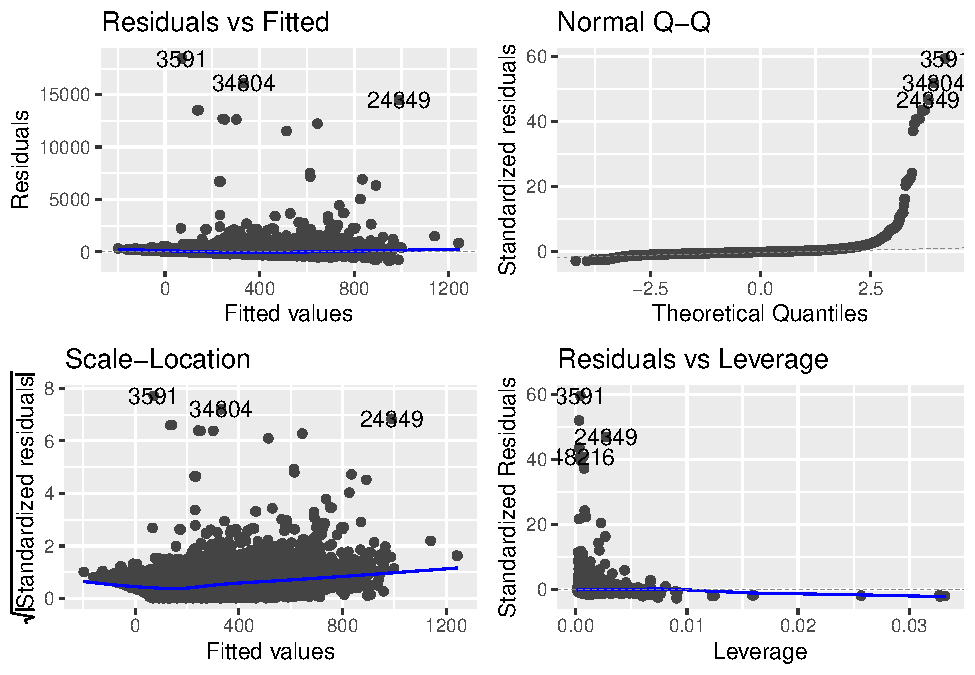
\includegraphics{Project_files/figure-latex/unnamed-chunk-24-1.png}

\begin{Shaded}
\begin{Highlighting}[]
\FunctionTok{ggplot}\NormalTok{(my\_data\_filtered, }\FunctionTok{aes}\NormalTok{(}\AttributeTok{x =}\NormalTok{ realSum, }\AttributeTok{y =}\NormalTok{ guest\_satisfaction\_overall,}
    \AttributeTok{color =}\NormalTok{ city\_day)) }\SpecialCharTok{+} \FunctionTok{geom\_point}\NormalTok{() }\SpecialCharTok{+} \FunctionTok{xlab}\NormalTok{(}\StringTok{"Price"}\NormalTok{) }\SpecialCharTok{+} \FunctionTok{ylab}\NormalTok{(}\StringTok{"Guest Satisfaction Overall"}\NormalTok{) }\SpecialCharTok{+}
    \FunctionTok{scale\_color\_discrete}\NormalTok{(}\AttributeTok{name =} \StringTok{"City{-}Day"}\NormalTok{) }\SpecialCharTok{+} \FunctionTok{facet\_wrap}\NormalTok{(}\SpecialCharTok{\textasciitilde{}}\NormalTok{city\_day)}
\end{Highlighting}
\end{Shaded}

\includegraphics{Project_files/figure-latex/unnamed-chunk-24-2.png}

The plot depicts that there is no correlation of price with guest
satisfaction, good satisfaction rate is found across all the prices. In
some cities like london, we can see a group of reviews with low guest
satisfaction.

\hypertarget{real-sum-vs-bedroom-count}{%
\subsubsection{Real Sum Vs Bedroom
Count}\label{real-sum-vs-bedroom-count}}

\begin{Shaded}
\begin{Highlighting}[]
\FunctionTok{ggplot}\NormalTok{(my\_data, }\FunctionTok{aes}\NormalTok{(}\AttributeTok{x =}\NormalTok{ realSum, }\AttributeTok{fill =}\NormalTok{ bedrooms, }\AttributeTok{group =}\NormalTok{ bedrooms)) }\SpecialCharTok{+}
    \FunctionTok{geom\_histogram}\NormalTok{(}\AttributeTok{alpha =} \FloatTok{0.6}\NormalTok{) }\SpecialCharTok{+} \FunctionTok{theme}\NormalTok{(}\AttributeTok{axis.title.x =} \FunctionTok{element\_text}\NormalTok{(}\AttributeTok{size =} \DecValTok{14}\NormalTok{),}
    \AttributeTok{axis.title.y =} \FunctionTok{element\_text}\NormalTok{(}\AttributeTok{size =} \DecValTok{14}\NormalTok{))}
\end{Highlighting}
\end{Shaded}

\includegraphics{Project_files/figure-latex/unnamed-chunk-25-1.png}

\begin{Shaded}
\begin{Highlighting}[]
\FunctionTok{ggplot}\NormalTok{(my\_data\_filtered, }\FunctionTok{aes}\NormalTok{(}\AttributeTok{x =}\NormalTok{ realSum, }\AttributeTok{fill =}\NormalTok{ bedrooms, }\AttributeTok{group =}\NormalTok{ bedrooms)) }\SpecialCharTok{+}
    \FunctionTok{geom\_histogram}\NormalTok{(}\AttributeTok{alpha =} \FloatTok{0.6}\NormalTok{) }\SpecialCharTok{+} \FunctionTok{theme}\NormalTok{(}\AttributeTok{axis.title.x =} \FunctionTok{element\_text}\NormalTok{(}\AttributeTok{size =} \DecValTok{14}\NormalTok{),}
    \AttributeTok{axis.title.y =} \FunctionTok{element\_text}\NormalTok{(}\AttributeTok{size =} \DecValTok{14}\NormalTok{))}
\end{Highlighting}
\end{Shaded}

\includegraphics{Project_files/figure-latex/unnamed-chunk-25-2.png}

\begin{Shaded}
\begin{Highlighting}[]
\FunctionTok{ggplot}\NormalTok{(my\_data\_filtered, }\FunctionTok{aes}\NormalTok{(}\AttributeTok{x =}\NormalTok{ realSum, }\AttributeTok{fill =}\NormalTok{ bedrooms, }\AttributeTok{group =}\NormalTok{ bedrooms)) }\SpecialCharTok{+}
    \FunctionTok{geom\_histogram}\NormalTok{(}\AttributeTok{alpha =} \FloatTok{0.6}\NormalTok{) }\SpecialCharTok{+} \FunctionTok{theme}\NormalTok{(}\AttributeTok{axis.title.x =} \FunctionTok{element\_text}\NormalTok{(}\AttributeTok{size =} \DecValTok{14}\NormalTok{),}
    \AttributeTok{axis.title.y =} \FunctionTok{element\_text}\NormalTok{(}\AttributeTok{size =} \DecValTok{14}\NormalTok{)) }\SpecialCharTok{+} \FunctionTok{facet\_wrap}\NormalTok{(}\SpecialCharTok{\textasciitilde{}}\NormalTok{city\_day)}
\end{Highlighting}
\end{Shaded}

\includegraphics{Project_files/figure-latex/unnamed-chunk-25-3.png}

\begin{Shaded}
\begin{Highlighting}[]
\FunctionTok{ggplot}\NormalTok{(my\_data\_filtered, }\FunctionTok{aes}\NormalTok{(}\AttributeTok{x =} \FunctionTok{reorder}\NormalTok{(city\_day, bedrooms,}
    \AttributeTok{FUN =}\NormalTok{ median), }\AttributeTok{y =}\NormalTok{ bedrooms, }\AttributeTok{fill =}\NormalTok{ city\_day)) }\SpecialCharTok{+} \FunctionTok{geom\_boxplot}\NormalTok{() }\SpecialCharTok{+}
    \FunctionTok{coord\_flip}\NormalTok{() }\SpecialCharTok{+} \FunctionTok{theme}\NormalTok{(}\AttributeTok{legend.key.height =} \FunctionTok{unit}\NormalTok{(}\FloatTok{0.5}\NormalTok{, }\StringTok{"cm"}\NormalTok{),}
    \AttributeTok{legend.key.size =} \FunctionTok{unit}\NormalTok{(}\DecValTok{1}\NormalTok{, }\StringTok{"lines"}\NormalTok{))}
\end{Highlighting}
\end{Shaded}

\includegraphics{Project_files/figure-latex/unnamed-chunk-26-1.png}

\begin{Shaded}
\begin{Highlighting}[]
\FunctionTok{cor}\NormalTok{(}\FunctionTok{as.numeric}\NormalTok{(}\FunctionTok{factor}\NormalTok{(my\_data}\SpecialCharTok{$}\NormalTok{multi)), }\FunctionTok{as.numeric}\NormalTok{(}\FunctionTok{factor}\NormalTok{(my\_data}\SpecialCharTok{$}\NormalTok{biz)))}
\end{Highlighting}
\end{Shaded}

\begin{verbatim}
## [1] -0.4707248
\end{verbatim}

\hypertarget{non-outlier-analysis}{%
\subsection{Non Outlier Analysis}\label{non-outlier-analysis}}

\hypertarget{boxplot-of-price-vs-city}{%
\subsubsection{Boxplot of Price Vs
City}\label{boxplot-of-price-vs-city}}

\begin{Shaded}
\begin{Highlighting}[]
\FunctionTok{ggplot}\NormalTok{(my\_data\_filtered, }\FunctionTok{aes}\NormalTok{(}\AttributeTok{x =} \FunctionTok{reorder}\NormalTok{(city\_day, realSum, }\AttributeTok{FUN =}\NormalTok{ median),}
    \AttributeTok{y =}\NormalTok{ realSum, }\AttributeTok{fill =}\NormalTok{ city\_day)) }\SpecialCharTok{+} \FunctionTok{geom\_boxplot}\NormalTok{() }\SpecialCharTok{+} \FunctionTok{coord\_flip}\NormalTok{() }\SpecialCharTok{+}
    \FunctionTok{theme}\NormalTok{(}\AttributeTok{legend.key.height =} \FunctionTok{unit}\NormalTok{(}\FloatTok{0.5}\NormalTok{, }\StringTok{"cm"}\NormalTok{), }\AttributeTok{legend.key.size =} \FunctionTok{unit}\NormalTok{(}\DecValTok{1}\NormalTok{,}
        \StringTok{"lines"}\NormalTok{))}
\end{Highlighting}
\end{Shaded}

\includegraphics{Project_files/figure-latex/unnamed-chunk-28-1.png}

The highest prices in Europe are found in Amsterdam.

\hypertarget{density-plot-of-price-vs-room-type}{%
\subsubsection{Density plot of Price vs Room
type}\label{density-plot-of-price-vs-room-type}}

\begin{Shaded}
\begin{Highlighting}[]
\FunctionTok{ggplot}\NormalTok{(my\_data\_filtered, }\FunctionTok{aes}\NormalTok{(}\AttributeTok{x =}\NormalTok{ realSum, }\AttributeTok{group =}\NormalTok{ room\_type,}
    \AttributeTok{fill =}\NormalTok{ room\_type, }\AttributeTok{alpha =} \FloatTok{0.2}\NormalTok{)) }\SpecialCharTok{+} \FunctionTok{geom\_density}\NormalTok{()}
\end{Highlighting}
\end{Shaded}

\includegraphics{Project_files/figure-latex/unnamed-chunk-29-1.png}

The prices of entire home are high comparatively

\hypertarget{scatterplot-of-prices-in-rome-w.r.t-latitude-and-longitude-during-weekdays}{%
\subsubsection{Scatterplot of Prices in Rome w.r.t Latitude and
Longitude during
weekdays}\label{scatterplot-of-prices-in-rome-w.r.t-latitude-and-longitude-during-weekdays}}

\begin{Shaded}
\begin{Highlighting}[]
\NormalTok{tema }\OtherTok{\textless{}{-}} \FunctionTok{theme}\NormalTok{(}\AttributeTok{plot.title =} \FunctionTok{element\_text}\NormalTok{(}\AttributeTok{size =} \DecValTok{23}\NormalTok{, }\AttributeTok{hjust =} \FloatTok{0.5}\NormalTok{),}
    \AttributeTok{axis.text.x =} \FunctionTok{element\_text}\NormalTok{(}\AttributeTok{size =} \DecValTok{19}\NormalTok{, }\AttributeTok{face =} \StringTok{"bold"}\NormalTok{), }\AttributeTok{axis.text.y =} \FunctionTok{element\_text}\NormalTok{(}\AttributeTok{size =} \DecValTok{19}\NormalTok{,}
        \AttributeTok{face =} \StringTok{"bold"}\NormalTok{), }\AttributeTok{axis.title.x =} \FunctionTok{element\_text}\NormalTok{(}\AttributeTok{size =} \DecValTok{19}\NormalTok{),}
    \AttributeTok{axis.title.y =} \FunctionTok{element\_text}\NormalTok{(}\AttributeTok{size =} \DecValTok{19}\NormalTok{), }\AttributeTok{legend.text =} \FunctionTok{element\_text}\NormalTok{(}\AttributeTok{colour =} \StringTok{"black"}\NormalTok{,}
        \AttributeTok{size =} \DecValTok{19}\NormalTok{, }\AttributeTok{face =} \StringTok{"bold"}\NormalTok{), }\AttributeTok{legend.background =} \FunctionTok{element\_rect}\NormalTok{(}\AttributeTok{fill =} \StringTok{"\#F5FFFA"}\NormalTok{,}
        \AttributeTok{size =} \FloatTok{0.5}\NormalTok{, }\AttributeTok{linetype =} \StringTok{"dashed"}\NormalTok{, }\AttributeTok{colour =} \StringTok{"black"}\NormalTok{))}

\NormalTok{rome\_data }\OtherTok{\textless{}{-}}\NormalTok{ my\_data\_filtered }\SpecialCharTok{\%\textgreater{}\%}
    \FunctionTok{subset}\NormalTok{(city\_day }\SpecialCharTok{==} \StringTok{"rome\_weekdays"}\NormalTok{)}

\FunctionTok{ggplot}\NormalTok{(}\AttributeTok{data =}\NormalTok{ rome\_data, }\AttributeTok{mapping =} \FunctionTok{aes}\NormalTok{(}\AttributeTok{x =}\NormalTok{ lat, }\AttributeTok{y =}\NormalTok{ lng)) }\SpecialCharTok{+} \FunctionTok{theme\_minimal}\NormalTok{() }\SpecialCharTok{+}
    \FunctionTok{scale\_fill\_identity}\NormalTok{() }\SpecialCharTok{+} \FunctionTok{geom\_point}\NormalTok{(}\AttributeTok{mapping =} \FunctionTok{aes}\NormalTok{(}\AttributeTok{color =}\NormalTok{ realSum),}
    \AttributeTok{size =} \DecValTok{3}\NormalTok{) }\SpecialCharTok{+} \FunctionTok{ggtitle}\NormalTok{(}\StringTok{""}\NormalTok{) }\SpecialCharTok{+}\NormalTok{ tema}
\end{Highlighting}
\end{Shaded}

\includegraphics{Project_files/figure-latex/unnamed-chunk-30-1.png}

This plot is within expectations of general trends, which suggests
similar types of establishments (price and hospitality) tend be in
clusters.

\hypertarget{attraction-index-in-all-cities}{%
\subsubsection{Attraction Index in all
Cities}\label{attraction-index-in-all-cities}}

\begin{Shaded}
\begin{Highlighting}[]
\CommentTok{\# create a new column that groups the cities}
\NormalTok{my\_data\_filtered}\SpecialCharTok{$}\NormalTok{city\_group }\OtherTok{\textless{}{-}} \FunctionTok{ifelse}\NormalTok{(my\_data\_filtered}\SpecialCharTok{$}\NormalTok{city\_day }\SpecialCharTok{\%in\%}
    \FunctionTok{c}\NormalTok{(}\StringTok{"amsterdam\_weekdays"}\NormalTok{, }\StringTok{"amsterdam\_weekends"}\NormalTok{), }\StringTok{"amsterdam"}\NormalTok{,}
    \FunctionTok{ifelse}\NormalTok{(my\_data\_filtered}\SpecialCharTok{$}\NormalTok{city\_day }\SpecialCharTok{\%in\%} \FunctionTok{c}\NormalTok{(}\StringTok{"athens\_weekdays"}\NormalTok{,}
        \StringTok{"athens\_weekends"}\NormalTok{), }\StringTok{"athens"}\NormalTok{, }\FunctionTok{ifelse}\NormalTok{(my\_data\_filtered}\SpecialCharTok{$}\NormalTok{city\_day }\SpecialCharTok{\%in\%}
        \FunctionTok{c}\NormalTok{(}\StringTok{"barcelona\_weekdays"}\NormalTok{, }\StringTok{"barcelona\_weekends"}\NormalTok{), }\StringTok{"barcelona"}\NormalTok{,}
        \FunctionTok{ifelse}\NormalTok{(my\_data\_filtered}\SpecialCharTok{$}\NormalTok{city\_day }\SpecialCharTok{\%in\%} \FunctionTok{c}\NormalTok{(}\StringTok{"berlin\_weekdays"}\NormalTok{,}
            \StringTok{"berlin\_weekends"}\NormalTok{), }\StringTok{"berlin"}\NormalTok{, }\FunctionTok{ifelse}\NormalTok{(my\_data\_filtered}\SpecialCharTok{$}\NormalTok{city\_day }\SpecialCharTok{\%in\%}
            \FunctionTok{c}\NormalTok{(}\StringTok{"budapest\_weekdays"}\NormalTok{, }\StringTok{"budapest\_weekends"}\NormalTok{), }\StringTok{"budapest"}\NormalTok{,}
            \FunctionTok{ifelse}\NormalTok{(my\_data\_filtered}\SpecialCharTok{$}\NormalTok{city\_day }\SpecialCharTok{\%in\%} \FunctionTok{c}\NormalTok{(}\StringTok{"lisbon\_weekdays"}\NormalTok{,}
                \StringTok{"lisbon\_weekends"}\NormalTok{), }\StringTok{"lisbon"}\NormalTok{, }\FunctionTok{ifelse}\NormalTok{(my\_data\_filtered}\SpecialCharTok{$}\NormalTok{city\_day }\SpecialCharTok{\%in\%}
                \FunctionTok{c}\NormalTok{(}\StringTok{"london\_weekdays"}\NormalTok{, }\StringTok{"london\_weekends"}\NormalTok{), }\StringTok{"london"}\NormalTok{,}
                \FunctionTok{ifelse}\NormalTok{(my\_data\_filtered}\SpecialCharTok{$}\NormalTok{city\_day }\SpecialCharTok{\%in\%} \FunctionTok{c}\NormalTok{(}\StringTok{"paris\_weekdays"}\NormalTok{,}
                  \StringTok{"paris\_weekends"}\NormalTok{), }\StringTok{"paris"}\NormalTok{, }\FunctionTok{ifelse}\NormalTok{(my\_data\_filtered}\SpecialCharTok{$}\NormalTok{city\_day }\SpecialCharTok{\%in\%}
                  \FunctionTok{c}\NormalTok{(}\StringTok{"rome\_weekdays"}\NormalTok{, }\StringTok{"rome\_weekends"}\NormalTok{), }\StringTok{"rome"}\NormalTok{,}
                  \StringTok{"vienna"}\NormalTok{)))))))))}

\CommentTok{\# plot the density plot with the new groupings}
\FunctionTok{ggplot}\NormalTok{(my\_data\_filtered, }\FunctionTok{aes}\NormalTok{(}\AttributeTok{x =}\NormalTok{ attr\_index\_norm, }\AttributeTok{fill =}\NormalTok{ city\_group,}
    \AttributeTok{alpha =} \FloatTok{0.2}\NormalTok{)) }\SpecialCharTok{+} \FunctionTok{geom\_density}\NormalTok{() }\SpecialCharTok{+} \FunctionTok{scale\_fill\_manual}\NormalTok{(}\AttributeTok{values =} \FunctionTok{c}\NormalTok{(}\AttributeTok{amsterdam =} \StringTok{"red"}\NormalTok{,}
    \AttributeTok{athens =} \StringTok{"blue"}\NormalTok{, }\AttributeTok{barcelona =} \StringTok{"green"}\NormalTok{, }\AttributeTok{berlin =} \StringTok{"orange"}\NormalTok{,}
    \AttributeTok{budapest =} \StringTok{"purple"}\NormalTok{, }\AttributeTok{lisbon =} \StringTok{"black"}\NormalTok{, }\AttributeTok{london =} \StringTok{"brown"}\NormalTok{,}
    \AttributeTok{paris =} \StringTok{"grey"}\NormalTok{, }\AttributeTok{rome =} \StringTok{"pink"}\NormalTok{, }\AttributeTok{vienna =} \StringTok{"yellow"}\NormalTok{)) }\SpecialCharTok{+} \FunctionTok{labs}\NormalTok{(}\AttributeTok{fill =} \StringTok{"City Group"}\NormalTok{)}
\end{Highlighting}
\end{Shaded}

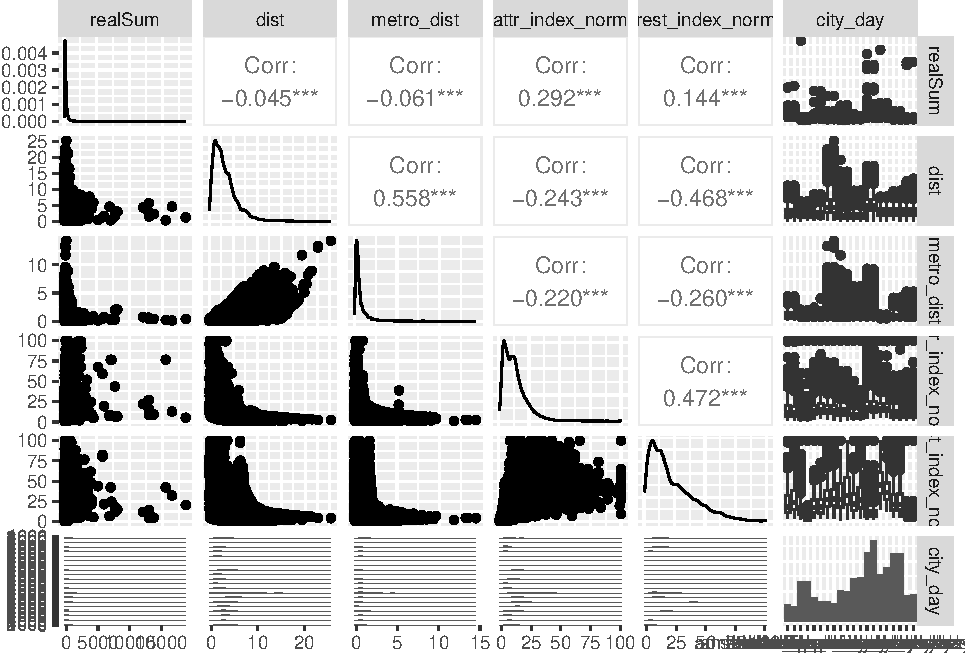
\includegraphics{Project_files/figure-latex/unnamed-chunk-31-1.png}

\hypertarget{real-sum-vs-room-shared-for-all-cities}{%
\subsection{Real Sum vs Room Shared for all
Cities}\label{real-sum-vs-room-shared-for-all-cities}}

\begin{Shaded}
\begin{Highlighting}[]
\FunctionTok{ggplot}\NormalTok{(my\_data\_filtered, }\FunctionTok{aes}\NormalTok{(}\AttributeTok{x =}\NormalTok{ room\_shared, }\AttributeTok{y =}\NormalTok{ realSum, }\AttributeTok{color =}\NormalTok{ city\_group),}
    \AttributeTok{alpha =} \FloatTok{0.001}\NormalTok{) }\SpecialCharTok{+} \FunctionTok{geom\_point}\NormalTok{() }\SpecialCharTok{+} \FunctionTok{scale\_fill\_manual}\NormalTok{(}\AttributeTok{values =} \FunctionTok{c}\NormalTok{(}\AttributeTok{amsterdam =} \StringTok{"red"}\NormalTok{,}
    \AttributeTok{athens =} \StringTok{"blue"}\NormalTok{, }\AttributeTok{barcelona =} \StringTok{"green"}\NormalTok{, }\AttributeTok{berlin =} \StringTok{"orange"}\NormalTok{,}
    \AttributeTok{budapest =} \StringTok{"purple"}\NormalTok{, }\AttributeTok{lisbon =} \StringTok{"black"}\NormalTok{, }\AttributeTok{london =} \StringTok{"brown"}\NormalTok{,}
    \AttributeTok{paris =} \StringTok{"grey"}\NormalTok{, }\AttributeTok{rome =} \StringTok{"pink"}\NormalTok{, }\AttributeTok{vienna =} \StringTok{"yellow"}\NormalTok{)) }\SpecialCharTok{+} \FunctionTok{labs}\NormalTok{(}\AttributeTok{fill =} \StringTok{"City Group"}\NormalTok{)}
\end{Highlighting}
\end{Shaded}

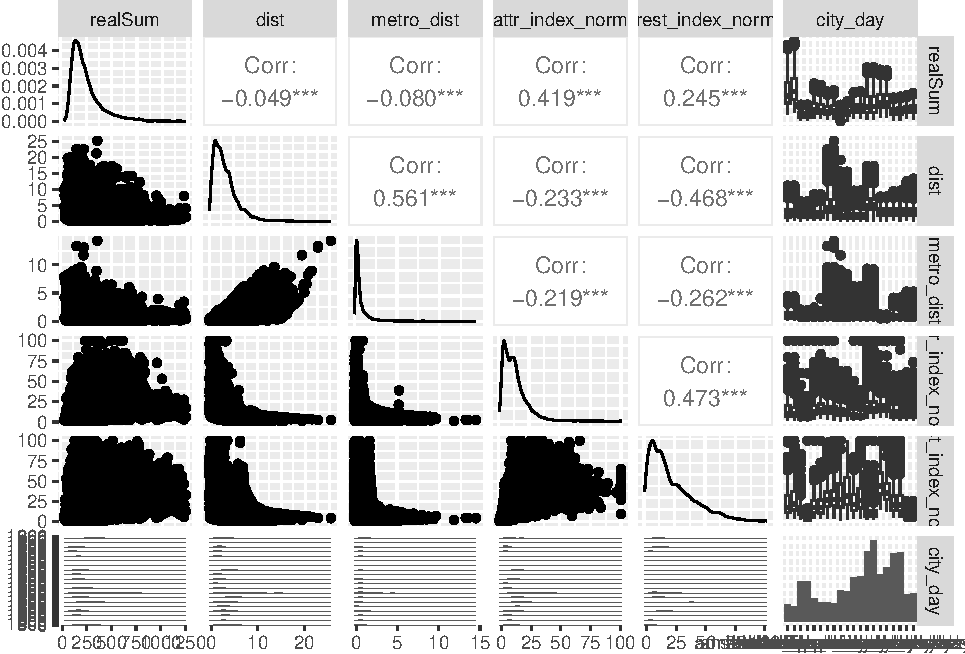
\includegraphics{Project_files/figure-latex/unnamed-chunk-32-1.png}

\hypertarget{different-model-selection-and-training}{%
\section{Different Model Selection and
Training}\label{different-model-selection-and-training}}

\hypertarget{checking-for-correlations-between-different-attributes}{%
\subsection{Checking for correlations between different
attributes}\label{checking-for-correlations-between-different-attributes}}

\begin{Shaded}
\begin{Highlighting}[]
\FunctionTok{ggpairs}\NormalTok{(my\_data[}\FunctionTok{c}\NormalTok{(}\StringTok{"realSum"}\NormalTok{, }\StringTok{"dist"}\NormalTok{, }\StringTok{"metro\_dist"}\NormalTok{, }\StringTok{"attr\_index\_norm"}\NormalTok{,}
    \StringTok{"rest\_index\_norm"}\NormalTok{, }\StringTok{"city\_day"}\NormalTok{)], }\AttributeTok{cardinality =} \DecValTok{20}\NormalTok{, }\AttributeTok{cardinality\_threshold =} \DecValTok{999}\NormalTok{)}
\end{Highlighting}
\end{Shaded}

\includegraphics{Project_files/figure-latex/unnamed-chunk-33-1.png}

\begin{Shaded}
\begin{Highlighting}[]
\FunctionTok{ggpairs}\NormalTok{(my\_data\_filtered[}\FunctionTok{c}\NormalTok{(}\StringTok{"realSum"}\NormalTok{, }\StringTok{"dist"}\NormalTok{, }\StringTok{"metro\_dist"}\NormalTok{, }\StringTok{"attr\_index\_norm"}\NormalTok{,}
    \StringTok{"rest\_index\_norm"}\NormalTok{, }\StringTok{"city\_day"}\NormalTok{)], }\AttributeTok{cardinality =} \DecValTok{20}\NormalTok{, }\AttributeTok{cardinality\_threshold =} \DecValTok{999}\NormalTok{)}
\end{Highlighting}
\end{Shaded}

\includegraphics{Project_files/figure-latex/unnamed-chunk-34-1.png}

\begin{Shaded}
\begin{Highlighting}[]
\FunctionTok{cor}\NormalTok{(my\_data}\SpecialCharTok{$}\NormalTok{attr\_index, my\_data}\SpecialCharTok{$}\NormalTok{rest\_index)}
\end{Highlighting}
\end{Shaded}

\begin{verbatim}
## [1] 0.4721427
\end{verbatim}

\begin{Shaded}
\begin{Highlighting}[]
\FunctionTok{ggplot}\NormalTok{() }\SpecialCharTok{+} \FunctionTok{geom\_point}\NormalTok{(}\AttributeTok{data =}\NormalTok{ my\_data\_filtered, }\FunctionTok{aes}\NormalTok{(}\AttributeTok{x =}\NormalTok{ attr\_index\_norm,}
    \AttributeTok{y =}\NormalTok{ rest\_index\_norm, }\AttributeTok{color =} \StringTok{"Filtered Data"}\NormalTok{), }\AttributeTok{alpha =} \FloatTok{0.4}\NormalTok{) }\SpecialCharTok{+}
    \FunctionTok{geom\_point}\NormalTok{(}\AttributeTok{data =}\NormalTok{ my\_outliers, }\FunctionTok{aes}\NormalTok{(}\AttributeTok{x =}\NormalTok{ attr\_index\_norm, }\AttributeTok{y =}\NormalTok{ rest\_index\_norm,}
        \AttributeTok{color =} \StringTok{"Outliers"}\NormalTok{), }\AttributeTok{alpha =} \FloatTok{0.4}\NormalTok{) }\SpecialCharTok{+} \FunctionTok{scale\_color\_manual}\NormalTok{(}\AttributeTok{values =} \FunctionTok{c}\NormalTok{(}\StringTok{\textasciigrave{}}\AttributeTok{Filtered Data}\StringTok{\textasciigrave{}} \OtherTok{=} \StringTok{"blue"}\NormalTok{,}
    \AttributeTok{Outliers =} \StringTok{"red"}\NormalTok{))}
\end{Highlighting}
\end{Shaded}

\includegraphics{Project_files/figure-latex/unnamed-chunk-36-1.png}

\begin{Shaded}
\begin{Highlighting}[]
\FunctionTok{ggplot}\NormalTok{() }\SpecialCharTok{+} \FunctionTok{geom\_point}\NormalTok{(}\AttributeTok{data =}\NormalTok{ my\_data\_filtered, }\FunctionTok{aes}\NormalTok{(}\AttributeTok{x =}\NormalTok{ attr\_index\_norm,}
    \AttributeTok{y =}\NormalTok{ rest\_index\_norm, }\AttributeTok{color =} \StringTok{"Filtered Data"}\NormalTok{), }\AttributeTok{alpha =} \FloatTok{0.4}\NormalTok{) }\SpecialCharTok{+}
    \FunctionTok{geom\_point}\NormalTok{(}\AttributeTok{data =}\NormalTok{ my\_outliers, }\FunctionTok{aes}\NormalTok{(}\AttributeTok{x =}\NormalTok{ attr\_index\_norm, }\AttributeTok{y =}\NormalTok{ rest\_index\_norm,}
        \AttributeTok{color =} \StringTok{"Outliers"}\NormalTok{), }\AttributeTok{alpha =} \FloatTok{0.4}\NormalTok{) }\SpecialCharTok{+} \FunctionTok{scale\_color\_manual}\NormalTok{(}\AttributeTok{values =} \FunctionTok{c}\NormalTok{(}\StringTok{\textasciigrave{}}\AttributeTok{Filtered Data}\StringTok{\textasciigrave{}} \OtherTok{=} \StringTok{"blue"}\NormalTok{,}
    \AttributeTok{Outliers =} \StringTok{"red"}\NormalTok{)) }\SpecialCharTok{+} \FunctionTok{facet\_wrap}\NormalTok{(}\SpecialCharTok{\textasciitilde{}}\NormalTok{city\_day)}
\end{Highlighting}
\end{Shaded}

\includegraphics{Project_files/figure-latex/unnamed-chunk-36-2.png}

\begin{Shaded}
\begin{Highlighting}[]
\FunctionTok{ggplot}\NormalTok{() }\SpecialCharTok{+} \FunctionTok{geom\_point}\NormalTok{(}\AttributeTok{data =}\NormalTok{ my\_data, }\FunctionTok{aes}\NormalTok{(}\AttributeTok{x =}\NormalTok{ attr\_index\_norm,}
    \AttributeTok{y =}\NormalTok{ rest\_index\_norm, }\AttributeTok{color =} \StringTok{"Filtered Data"}\NormalTok{), }\AttributeTok{alpha =} \FloatTok{0.4}\NormalTok{) }\SpecialCharTok{+}
    \FunctionTok{scale\_color\_manual}\NormalTok{(}\AttributeTok{values =} \FunctionTok{c}\NormalTok{(}\StringTok{\textasciigrave{}}\AttributeTok{Filtered Data}\StringTok{\textasciigrave{}} \OtherTok{=} \StringTok{"blue"}\NormalTok{))}
\end{Highlighting}
\end{Shaded}

\includegraphics{Project_files/figure-latex/unnamed-chunk-36-3.png}

\begin{Shaded}
\begin{Highlighting}[]
\FunctionTok{ggplot}\NormalTok{() }\SpecialCharTok{+} \FunctionTok{geom\_point}\NormalTok{(}\AttributeTok{data =}\NormalTok{ my\_data, }\FunctionTok{aes}\NormalTok{(}\AttributeTok{x =}\NormalTok{ attr\_index\_norm,}
    \AttributeTok{y =}\NormalTok{ rest\_index\_norm, }\AttributeTok{color =} \StringTok{"Filtered Data"}\NormalTok{), }\AttributeTok{alpha =} \FloatTok{0.4}\NormalTok{) }\SpecialCharTok{+}
    \FunctionTok{scale\_color\_manual}\NormalTok{(}\AttributeTok{values =} \FunctionTok{c}\NormalTok{(}\StringTok{\textasciigrave{}}\AttributeTok{Filtered Data}\StringTok{\textasciigrave{}} \OtherTok{=} \StringTok{"blue"}\NormalTok{)) }\SpecialCharTok{+}
    \FunctionTok{facet\_wrap}\NormalTok{(}\SpecialCharTok{\textasciitilde{}}\NormalTok{city\_day)}
\end{Highlighting}
\end{Shaded}

\includegraphics{Project_files/figure-latex/unnamed-chunk-36-4.png}

\begin{Shaded}
\begin{Highlighting}[]
\FunctionTok{cor}\NormalTok{(my\_data}\SpecialCharTok{$}\NormalTok{attr\_index\_norm, my\_data}\SpecialCharTok{$}\NormalTok{rest\_index\_norm)}
\end{Highlighting}
\end{Shaded}

\begin{verbatim}
## [1] 0.4721427
\end{verbatim}

\hypertarget{linear-polynomial-and-step-regression}{%
\subsection{Linear, Polynomial and Step
Regression}\label{linear-polynomial-and-step-regression}}

\hypertarget{mlr-seperated-by-city-day}{%
\subsubsection{MLR Seperated by City
Day}\label{mlr-seperated-by-city-day}}

\begin{Shaded}
\begin{Highlighting}[]
\NormalTok{temp\_data }\OtherTok{\textless{}{-}} \FunctionTok{subset}\NormalTok{(my\_data\_train, city\_day }\SpecialCharTok{==} \StringTok{"amsterdam\_weekends"} \SpecialCharTok{|}
\NormalTok{    city\_day }\SpecialCharTok{==} \StringTok{"amsterdam\_weekdays"}\NormalTok{)}

\NormalTok{M\_0 }\OtherTok{\textless{}{-}} \FunctionTok{lm}\NormalTok{(realSum }\SpecialCharTok{\textasciitilde{}}\NormalTok{ . }\SpecialCharTok{{-}}\NormalTok{ realSum }\SpecialCharTok{{-}}\NormalTok{ X, }\AttributeTok{data =}\NormalTok{ temp\_data)}
\NormalTok{temp\_data }\OtherTok{\textless{}{-}} \FunctionTok{subset}\NormalTok{(my\_data\_train, city\_day }\SpecialCharTok{==} \StringTok{"athens\_weekdays"} \SpecialCharTok{|}
\NormalTok{    city\_day }\SpecialCharTok{==} \StringTok{"athens\_weekends"}\NormalTok{, )}

\NormalTok{M\_1 }\OtherTok{\textless{}{-}} \FunctionTok{lm}\NormalTok{(realSum }\SpecialCharTok{\textasciitilde{}}\NormalTok{ . }\SpecialCharTok{{-}}\NormalTok{ realSum }\SpecialCharTok{{-}}\NormalTok{ X }\SpecialCharTok{{-}}\NormalTok{ city\_day, }\AttributeTok{data =}\NormalTok{ temp\_data)}
\NormalTok{temp\_data }\OtherTok{\textless{}{-}} \FunctionTok{subset}\NormalTok{(my\_data\_train, city\_day }\SpecialCharTok{==} \StringTok{"barcelona\_weekdays"} \SpecialCharTok{|}
\NormalTok{    city\_day }\SpecialCharTok{==} \StringTok{"barcelona\_weekends"}\NormalTok{, )}

\NormalTok{M\_2 }\OtherTok{\textless{}{-}} \FunctionTok{lm}\NormalTok{(realSum }\SpecialCharTok{\textasciitilde{}}\NormalTok{ . }\SpecialCharTok{{-}}\NormalTok{ realSum }\SpecialCharTok{{-}}\NormalTok{ X }\SpecialCharTok{{-}}\NormalTok{ city\_day, }\AttributeTok{data =}\NormalTok{ temp\_data)}
\NormalTok{temp\_data }\OtherTok{\textless{}{-}} \FunctionTok{subset}\NormalTok{(my\_data\_train, city\_day }\SpecialCharTok{==} \StringTok{"berlin\_weekdays"} \SpecialCharTok{|}
\NormalTok{    city\_day }\SpecialCharTok{==} \StringTok{"berlin\_weekends"}\NormalTok{, )}

\NormalTok{M\_3 }\OtherTok{\textless{}{-}} \FunctionTok{lm}\NormalTok{(realSum }\SpecialCharTok{\textasciitilde{}}\NormalTok{ . }\SpecialCharTok{{-}}\NormalTok{ realSum }\SpecialCharTok{{-}}\NormalTok{ X }\SpecialCharTok{{-}}\NormalTok{ city\_day, }\AttributeTok{data =}\NormalTok{ temp\_data)}
\NormalTok{temp\_data }\OtherTok{\textless{}{-}} \FunctionTok{subset}\NormalTok{(my\_data\_train, city\_day }\SpecialCharTok{==} \StringTok{"budapest\_weekdays"} \SpecialCharTok{|}
\NormalTok{    city\_day }\SpecialCharTok{==} \StringTok{"budapest\_weekends"}\NormalTok{, )}

\NormalTok{M\_4 }\OtherTok{\textless{}{-}} \FunctionTok{lm}\NormalTok{(realSum }\SpecialCharTok{\textasciitilde{}}\NormalTok{ . }\SpecialCharTok{{-}}\NormalTok{ realSum }\SpecialCharTok{{-}}\NormalTok{ X }\SpecialCharTok{{-}}\NormalTok{ city\_day, }\AttributeTok{data =}\NormalTok{ temp\_data)}
\NormalTok{temp\_data }\OtherTok{\textless{}{-}} \FunctionTok{subset}\NormalTok{(my\_data\_train, city\_day }\SpecialCharTok{==} \StringTok{"lisbon\_weekdays"} \SpecialCharTok{|}
\NormalTok{    city\_day }\SpecialCharTok{==} \StringTok{"lisbon\_weekends"}\NormalTok{, )}

\NormalTok{M\_5 }\OtherTok{\textless{}{-}} \FunctionTok{lm}\NormalTok{(realSum }\SpecialCharTok{\textasciitilde{}}\NormalTok{ . }\SpecialCharTok{{-}}\NormalTok{ realSum }\SpecialCharTok{{-}}\NormalTok{ X }\SpecialCharTok{{-}}\NormalTok{ city\_day, }\AttributeTok{data =}\NormalTok{ temp\_data)}
\NormalTok{temp\_data }\OtherTok{\textless{}{-}} \FunctionTok{subset}\NormalTok{(my\_data\_train, city\_day }\SpecialCharTok{==} \StringTok{"london\_weekdays"} \SpecialCharTok{|}
\NormalTok{    city\_day }\SpecialCharTok{==} \StringTok{"london\_weekends"}\NormalTok{, )}

\NormalTok{M\_6 }\OtherTok{\textless{}{-}} \FunctionTok{lm}\NormalTok{(realSum }\SpecialCharTok{\textasciitilde{}}\NormalTok{ . }\SpecialCharTok{{-}}\NormalTok{ realSum }\SpecialCharTok{{-}}\NormalTok{ X }\SpecialCharTok{{-}}\NormalTok{ city\_day, }\AttributeTok{data =}\NormalTok{ temp\_data)}
\NormalTok{temp\_data }\OtherTok{\textless{}{-}} \FunctionTok{subset}\NormalTok{(my\_data\_train, city\_day }\SpecialCharTok{==} \StringTok{"paris\_weekdays"} \SpecialCharTok{|}
\NormalTok{    city\_day }\SpecialCharTok{==} \StringTok{"paris\_weekends"}\NormalTok{, )}

\NormalTok{M\_7 }\OtherTok{\textless{}{-}} \FunctionTok{lm}\NormalTok{(realSum }\SpecialCharTok{\textasciitilde{}}\NormalTok{ . }\SpecialCharTok{{-}}\NormalTok{ realSum }\SpecialCharTok{{-}}\NormalTok{ X }\SpecialCharTok{{-}}\NormalTok{ city\_day, }\AttributeTok{data =}\NormalTok{ temp\_data)}
\NormalTok{temp\_data }\OtherTok{\textless{}{-}} \FunctionTok{subset}\NormalTok{(my\_data\_train, city\_day }\SpecialCharTok{==} \StringTok{"rome\_weekdays"} \SpecialCharTok{|}
\NormalTok{    city\_day }\SpecialCharTok{==} \StringTok{"rome\_weekends"}\NormalTok{, )}

\NormalTok{M\_8 }\OtherTok{\textless{}{-}} \FunctionTok{lm}\NormalTok{(realSum }\SpecialCharTok{\textasciitilde{}}\NormalTok{ . }\SpecialCharTok{{-}}\NormalTok{ realSum }\SpecialCharTok{{-}}\NormalTok{ X }\SpecialCharTok{{-}}\NormalTok{ city\_day, }\AttributeTok{data =}\NormalTok{ temp\_data)}
\NormalTok{temp\_data }\OtherTok{\textless{}{-}} \FunctionTok{subset}\NormalTok{(my\_data\_train, city\_day }\SpecialCharTok{==} \StringTok{"vienna\_weekdays"} \SpecialCharTok{|}
\NormalTok{    city\_day }\SpecialCharTok{==} \StringTok{"vienna\_weekends"}\NormalTok{, )}

\NormalTok{M\_9 }\OtherTok{\textless{}{-}} \FunctionTok{lm}\NormalTok{(realSum }\SpecialCharTok{\textasciitilde{}}\NormalTok{ . }\SpecialCharTok{{-}}\NormalTok{ realSum }\SpecialCharTok{{-}}\NormalTok{ X }\SpecialCharTok{{-}}\NormalTok{ city\_day, }\AttributeTok{data =}\NormalTok{ temp\_data)}
\end{Highlighting}
\end{Shaded}

\begin{Shaded}
\begin{Highlighting}[]
\NormalTok{coefs }\OtherTok{\textless{}{-}} \FunctionTok{tidy}\NormalTok{(M\_0)}
\NormalTok{coefs[}\FunctionTok{order}\NormalTok{(coefs}\SpecialCharTok{$}\NormalTok{estimate, }\AttributeTok{decreasing =} \ConstantTok{TRUE}\NormalTok{), ]}
\NormalTok{coefs }\OtherTok{\textless{}{-}} \FunctionTok{tidy}\NormalTok{(M\_1)}
\NormalTok{coefs[}\FunctionTok{order}\NormalTok{(coefs}\SpecialCharTok{$}\NormalTok{estimate, }\AttributeTok{decreasing =} \ConstantTok{TRUE}\NormalTok{), ]}
\NormalTok{coefs }\OtherTok{\textless{}{-}} \FunctionTok{tidy}\NormalTok{(M\_2)}
\NormalTok{coefs[}\FunctionTok{order}\NormalTok{(coefs}\SpecialCharTok{$}\NormalTok{estimate, }\AttributeTok{decreasing =} \ConstantTok{TRUE}\NormalTok{), ]}
\NormalTok{coefs }\OtherTok{\textless{}{-}} \FunctionTok{tidy}\NormalTok{(M\_3)}
\NormalTok{coefs[}\FunctionTok{order}\NormalTok{(coefs}\SpecialCharTok{$}\NormalTok{estimate, }\AttributeTok{decreasing =} \ConstantTok{TRUE}\NormalTok{), ]}
\NormalTok{coefs }\OtherTok{\textless{}{-}} \FunctionTok{tidy}\NormalTok{(M\_4)}
\NormalTok{coefs[}\FunctionTok{order}\NormalTok{(coefs}\SpecialCharTok{$}\NormalTok{estimate, }\AttributeTok{decreasing =} \ConstantTok{TRUE}\NormalTok{), ]}
\NormalTok{coefs }\OtherTok{\textless{}{-}} \FunctionTok{tidy}\NormalTok{(M\_5)}
\NormalTok{coefs[}\FunctionTok{order}\NormalTok{(coefs}\SpecialCharTok{$}\NormalTok{estimate, }\AttributeTok{decreasing =} \ConstantTok{TRUE}\NormalTok{), ]}
\NormalTok{coefs }\OtherTok{\textless{}{-}} \FunctionTok{tidy}\NormalTok{(M\_6)}
\NormalTok{coefs[}\FunctionTok{order}\NormalTok{(coefs}\SpecialCharTok{$}\NormalTok{estimate, }\AttributeTok{decreasing =} \ConstantTok{TRUE}\NormalTok{), ]}
\NormalTok{coefs }\OtherTok{\textless{}{-}} \FunctionTok{tidy}\NormalTok{(M\_7)}
\NormalTok{coefs[}\FunctionTok{order}\NormalTok{(coefs}\SpecialCharTok{$}\NormalTok{estimate, }\AttributeTok{decreasing =} \ConstantTok{TRUE}\NormalTok{), ]}
\NormalTok{coefs }\OtherTok{\textless{}{-}} \FunctionTok{tidy}\NormalTok{(M\_8)}
\NormalTok{coefs[}\FunctionTok{order}\NormalTok{(coefs}\SpecialCharTok{$}\NormalTok{estimate, }\AttributeTok{decreasing =} \ConstantTok{TRUE}\NormalTok{), ]}
\NormalTok{coefs }\OtherTok{\textless{}{-}} \FunctionTok{tidy}\NormalTok{(M\_9)}
\end{Highlighting}
\end{Shaded}

\begin{Shaded}
\begin{Highlighting}[]
\NormalTok{coefs[}\FunctionTok{order}\NormalTok{(coefs}\SpecialCharTok{$}\NormalTok{estimate, }\AttributeTok{decreasing =} \ConstantTok{TRUE}\NormalTok{), ]}
\end{Highlighting}
\end{Shaded}

\hypertarget{mlr}{%
\subsubsection{MLR}\label{mlr}}

\begin{Shaded}
\begin{Highlighting}[]
\NormalTok{M1 }\OtherTok{\textless{}{-}} \FunctionTok{lm}\NormalTok{(realSum }\SpecialCharTok{\textasciitilde{}}\NormalTok{ . }\SpecialCharTok{{-}}\NormalTok{ realSum }\SpecialCharTok{{-}}\NormalTok{ X, }\AttributeTok{data =}\NormalTok{ my\_data\_train)}
\end{Highlighting}
\end{Shaded}

\begin{Shaded}
\begin{Highlighting}[]
\FunctionTok{summary}\NormalTok{(M1)}
\end{Highlighting}
\end{Shaded}

\begin{verbatim}
## 
## Call:
## lm(formula = realSum ~ . - realSum - X, data = my_data_train)
## 
## Residuals:
##     Min      1Q  Median      3Q     Max 
##  -758.3   -84.0   -21.0    42.9 18422.4 
## 
## Coefficients:
##                              Estimate Std. Error t value Pr(>|t|)    
## (Intercept)                -4954.9076  3996.1824  -1.240 0.215017    
## room_typePrivate room       -114.3655     4.2823 -26.707  < 2e-16 ***
## room_typeShared room        -204.1842    18.9348 -10.784  < 2e-16 ***
## person_capacity               23.9626     1.7645  13.581  < 2e-16 ***
## host_is_superhostTrue          1.0749     3.9344   0.273 0.784700    
## multi                          9.6004     4.1324   2.323 0.020173 *  
## biz                           33.2806     4.1885   7.946 1.99e-15 ***
## cleanliness_rating             5.0383     2.4153   2.086 0.036987 *  
## guest_satisfaction_overall     0.7760     0.2615   2.968 0.002999 ** 
## bedrooms                      86.0154     3.1888  26.974  < 2e-16 ***
## dist                          -1.5330     1.2628  -1.214 0.224761    
## metro_dist                    -3.9967     2.5025  -1.597 0.110262    
## attr_index_norm                6.3705     0.2946  21.627  < 2e-16 ***
## rest_index_norm               -0.1837     0.1774  -1.036 0.300215    
## lng                         -262.8909    40.1931  -6.541 6.20e-11 ***
## lat                          123.2117    76.5228   1.610 0.107378    
## city_dayamsterdam_weekends    67.9410    16.0017   4.246 2.18e-05 ***
## city_dayathens_weekdays     6315.0906  1388.5351   4.548 5.43e-06 ***
## city_dayathens_weekends     6303.5311  1388.6527   4.539 5.66e-06 ***
## city_daybarcelona_weekdays   411.7717   837.7909   0.491 0.623078    
## city_daybarcelona_weekends   429.6529   837.8109   0.513 0.608075    
## city_dayberlin_weekdays     1949.0424   342.1245   5.697 1.23e-08 ***
## city_dayberlin_weekends     1958.8844   342.0401   5.727 1.03e-08 ***
## city_daybudapest_weekdays   3902.3511   706.8806   5.521 3.40e-08 ***
## city_daybudapest_weekends   3929.6734   706.8440   5.559 2.73e-08 ***
## city_daylisbon_weekdays    -2312.9309  1143.8977  -2.022 0.043186 *  
## city_daylisbon_weekends    -2304.0067  1143.8126  -2.014 0.043983 *  
## city_daylondon_weekdays    -1409.2997   206.1046  -6.838 8.17e-12 ***
## city_daylondon_weekends    -1410.9328   206.1223  -6.845 7.76e-12 ***
## city_dayparis_weekdays      -403.0289   278.4819  -1.447 0.147840    
## city_dayparis_weekends      -422.1389   278.6437  -1.515 0.129787    
## city_dayrome_weekdays       2947.6852   881.3984   3.344 0.000826 ***
## city_dayrome_weekends       2952.5352   881.4297   3.350 0.000810 ***
## city_dayvienna_weekdays     3231.8185   582.7092   5.546 2.94e-08 ***
## city_dayvienna_weekends     3230.2680   582.7972   5.543 3.00e-08 ***
## ---
## Signif. codes:  0 '***' 0.001 '**' 0.01 '*' 0.05 '.' 0.1 ' ' 1
## 
## Residual standard error: 305.1 on 36159 degrees of freedom
## Multiple R-squared:  0.215,  Adjusted R-squared:  0.2143 
## F-statistic: 291.3 on 34 and 36159 DF,  p-value: < 2.2e-16
\end{verbatim}

\begin{Shaded}
\begin{Highlighting}[]
\CommentTok{\# Create summary table with coefficients and p{-}values}
\NormalTok{table }\OtherTok{\textless{}{-}} \FunctionTok{summary}\NormalTok{(M1)}\SpecialCharTok{$}\NormalTok{coefficients[, }\FunctionTok{c}\NormalTok{(}\DecValTok{1}\NormalTok{, }\DecValTok{4}\NormalTok{)]}
\end{Highlighting}
\end{Shaded}

\begin{Shaded}
\begin{Highlighting}[]
\CommentTok{\# Calculate R{-}squared and multiple R{-}squared}
\NormalTok{y\_train\_pred }\OtherTok{\textless{}{-}} \FunctionTok{predict}\NormalTok{(M1, my\_data\_train)}
\NormalTok{y\_train\_mean }\OtherTok{\textless{}{-}} \FunctionTok{mean}\NormalTok{(my\_data\_train}\SpecialCharTok{$}\NormalTok{realSum)}
\NormalTok{SST }\OtherTok{\textless{}{-}} \FunctionTok{sum}\NormalTok{((my\_data\_train}\SpecialCharTok{$}\NormalTok{realSum }\SpecialCharTok{{-}}\NormalTok{ y\_train\_mean)}\SpecialCharTok{\^{}}\DecValTok{2}\NormalTok{)}
\NormalTok{SSR }\OtherTok{\textless{}{-}} \FunctionTok{sum}\NormalTok{((my\_data\_train}\SpecialCharTok{$}\NormalTok{realSum }\SpecialCharTok{{-}}\NormalTok{ y\_train\_pred)}\SpecialCharTok{\^{}}\DecValTok{2}\NormalTok{)}
\NormalTok{R\_squared }\OtherTok{\textless{}{-}} \DecValTok{1} \SpecialCharTok{{-}}\NormalTok{ SSR}\SpecialCharTok{/}\NormalTok{SST}
\NormalTok{n }\OtherTok{\textless{}{-}} \FunctionTok{length}\NormalTok{(my\_data\_train}\SpecialCharTok{$}\NormalTok{realSum)}
\NormalTok{p }\OtherTok{\textless{}{-}} \FunctionTok{ncol}\NormalTok{(my\_data\_train)}
\NormalTok{adj\_R\_squared }\OtherTok{\textless{}{-}} \DecValTok{1} \SpecialCharTok{{-}}\NormalTok{ (SSR}\SpecialCharTok{/}\NormalTok{(n }\SpecialCharTok{{-}}\NormalTok{ p }\SpecialCharTok{{-}} \DecValTok{1}\NormalTok{))}\SpecialCharTok{/}\NormalTok{(SST}\SpecialCharTok{/}\NormalTok{(n }\SpecialCharTok{{-}} \DecValTok{1}\NormalTok{))}
\NormalTok{RMSE }\OtherTok{=} \FunctionTok{sqrt}\NormalTok{(}\FunctionTok{mean}\NormalTok{((my\_data\_train}\SpecialCharTok{$}\NormalTok{realSum }\SpecialCharTok{{-}}\NormalTok{ y\_train\_pred)}\SpecialCharTok{\^{}}\DecValTok{2}\NormalTok{))}


\CommentTok{\# Print the R{-}squared and multiple R{-}squared values}
\FunctionTok{cat}\NormalTok{(}\StringTok{"R{-}squared:"}\NormalTok{, R\_squared, }\StringTok{"}\SpecialCharTok{\textbackslash{}n}\StringTok{"}\NormalTok{)}
\end{Highlighting}
\end{Shaded}

\begin{verbatim}
## R-squared: 0.2150414
\end{verbatim}

\begin{Shaded}
\begin{Highlighting}[]
\FunctionTok{cat}\NormalTok{(}\StringTok{"Adjusted R{-}squared:"}\NormalTok{, adj\_R\_squared, }\StringTok{"}\SpecialCharTok{\textbackslash{}n}\StringTok{"}\NormalTok{)}
\end{Highlighting}
\end{Shaded}

\begin{verbatim}
## Adjusted R-squared: 0.2146725
\end{verbatim}

\begin{Shaded}
\begin{Highlighting}[]
\FunctionTok{cat}\NormalTok{(}\StringTok{"RMSE:"}\NormalTok{, RMSE, }\StringTok{"}\SpecialCharTok{\textbackslash{}n}\StringTok{"}\NormalTok{)}
\end{Highlighting}
\end{Shaded}

\begin{verbatim}
## RMSE: 304.9175
\end{verbatim}

The r\^{}2 and adjusted r\^{}2 values are too low for the Linear
regression model to be considered a competent one in this case.

\begin{Shaded}
\begin{Highlighting}[]
\CommentTok{\# Calculate R{-}squared and multiple R{-}squared}
\NormalTok{y\_train\_pred }\OtherTok{\textless{}{-}} \FunctionTok{predict}\NormalTok{(M1, my\_data\_test)}
\NormalTok{y\_train\_mean }\OtherTok{\textless{}{-}} \FunctionTok{mean}\NormalTok{(my\_data\_test}\SpecialCharTok{$}\NormalTok{realSum)}
\NormalTok{SST }\OtherTok{\textless{}{-}} \FunctionTok{sum}\NormalTok{((my\_data\_test}\SpecialCharTok{$}\NormalTok{realSum }\SpecialCharTok{{-}}\NormalTok{ y\_train\_mean)}\SpecialCharTok{\^{}}\DecValTok{2}\NormalTok{)}
\NormalTok{SSR }\OtherTok{\textless{}{-}} \FunctionTok{sum}\NormalTok{((my\_data\_test}\SpecialCharTok{$}\NormalTok{realSum }\SpecialCharTok{{-}}\NormalTok{ y\_train\_pred)}\SpecialCharTok{\^{}}\DecValTok{2}\NormalTok{)}
\NormalTok{R\_squared }\OtherTok{\textless{}{-}} \DecValTok{1} \SpecialCharTok{{-}}\NormalTok{ SSR}\SpecialCharTok{/}\NormalTok{SST}
\NormalTok{n }\OtherTok{\textless{}{-}} \FunctionTok{length}\NormalTok{(my\_data\_test}\SpecialCharTok{$}\NormalTok{realSum)}
\NormalTok{p }\OtherTok{\textless{}{-}} \FunctionTok{ncol}\NormalTok{(my\_data\_test)}
\NormalTok{adj\_R\_squared }\OtherTok{\textless{}{-}} \DecValTok{1} \SpecialCharTok{{-}}\NormalTok{ (SSR}\SpecialCharTok{/}\NormalTok{(n }\SpecialCharTok{{-}}\NormalTok{ p }\SpecialCharTok{{-}} \DecValTok{1}\NormalTok{))}\SpecialCharTok{/}\NormalTok{(SST}\SpecialCharTok{/}\NormalTok{(n }\SpecialCharTok{{-}} \DecValTok{1}\NormalTok{))}
\NormalTok{RMSE }\OtherTok{=} \FunctionTok{sqrt}\NormalTok{(}\FunctionTok{mean}\NormalTok{((my\_data\_test}\SpecialCharTok{$}\NormalTok{realSum }\SpecialCharTok{{-}}\NormalTok{ y\_train\_pred)}\SpecialCharTok{\^{}}\DecValTok{2}\NormalTok{))}


\CommentTok{\# Print the R{-}squared and multiple R{-}squared values}
\FunctionTok{cat}\NormalTok{(}\StringTok{"R{-}squared:"}\NormalTok{, R\_squared, }\StringTok{"}\SpecialCharTok{\textbackslash{}n}\StringTok{"}\NormalTok{)}
\end{Highlighting}
\end{Shaded}

\begin{verbatim}
## R-squared: 0.33744
\end{verbatim}

\begin{Shaded}
\begin{Highlighting}[]
\FunctionTok{cat}\NormalTok{(}\StringTok{"Adjusted R{-}squared:"}\NormalTok{, adj\_R\_squared, }\StringTok{"}\SpecialCharTok{\textbackslash{}n}\StringTok{"}\NormalTok{)}
\end{Highlighting}
\end{Shaded}

\begin{verbatim}
## Adjusted R-squared: 0.3367131
\end{verbatim}

\begin{Shaded}
\begin{Highlighting}[]
\FunctionTok{cat}\NormalTok{(}\StringTok{"RMSE:"}\NormalTok{, RMSE, }\StringTok{"}\SpecialCharTok{\textbackslash{}n}\StringTok{"}\NormalTok{)}
\end{Highlighting}
\end{Shaded}

\begin{verbatim}
## RMSE: 233.2618
\end{verbatim}

\begin{Shaded}
\begin{Highlighting}[]
\NormalTok{M1\_step }\OtherTok{=} \FunctionTok{step}\NormalTok{(M1, }\AttributeTok{direction =} \StringTok{"backward"}\NormalTok{)}
\end{Highlighting}
\end{Shaded}

\begin{Shaded}
\begin{Highlighting}[]
\CommentTok{\# Calculate R{-}squared and multiple R{-}squared}
\NormalTok{y\_train\_pred }\OtherTok{\textless{}{-}} \FunctionTok{predict}\NormalTok{(M1\_step, my\_data\_train)}
\NormalTok{y\_train\_mean }\OtherTok{\textless{}{-}} \FunctionTok{mean}\NormalTok{(my\_data\_train}\SpecialCharTok{$}\NormalTok{realSum)}
\NormalTok{SST }\OtherTok{\textless{}{-}} \FunctionTok{sum}\NormalTok{((my\_data\_train}\SpecialCharTok{$}\NormalTok{realSum }\SpecialCharTok{{-}}\NormalTok{ y\_train\_mean)}\SpecialCharTok{\^{}}\DecValTok{2}\NormalTok{)}
\NormalTok{SSR }\OtherTok{\textless{}{-}} \FunctionTok{sum}\NormalTok{((my\_data\_train}\SpecialCharTok{$}\NormalTok{realSum }\SpecialCharTok{{-}}\NormalTok{ y\_train\_pred)}\SpecialCharTok{\^{}}\DecValTok{2}\NormalTok{)}
\NormalTok{R\_squared }\OtherTok{\textless{}{-}} \DecValTok{1} \SpecialCharTok{{-}}\NormalTok{ SSR}\SpecialCharTok{/}\NormalTok{SST}
\NormalTok{n }\OtherTok{\textless{}{-}} \FunctionTok{length}\NormalTok{(my\_data\_train}\SpecialCharTok{$}\NormalTok{realSum)}
\NormalTok{p }\OtherTok{\textless{}{-}} \FunctionTok{ncol}\NormalTok{(my\_data\_train)}
\NormalTok{adj\_R\_squared }\OtherTok{\textless{}{-}} \DecValTok{1} \SpecialCharTok{{-}}\NormalTok{ (SSR}\SpecialCharTok{/}\NormalTok{(n }\SpecialCharTok{{-}}\NormalTok{ p }\SpecialCharTok{{-}} \DecValTok{1}\NormalTok{))}\SpecialCharTok{/}\NormalTok{(SST}\SpecialCharTok{/}\NormalTok{(n }\SpecialCharTok{{-}} \DecValTok{1}\NormalTok{))}
\NormalTok{RMSE }\OtherTok{=} \FunctionTok{sqrt}\NormalTok{(}\FunctionTok{mean}\NormalTok{((my\_data\_train}\SpecialCharTok{$}\NormalTok{realSum }\SpecialCharTok{{-}}\NormalTok{ y\_train\_pred)}\SpecialCharTok{\^{}}\DecValTok{2}\NormalTok{))}


\CommentTok{\# Print the R{-}squared and multiple R{-}squared values}
\FunctionTok{cat}\NormalTok{(}\StringTok{"R{-}squared:"}\NormalTok{, R\_squared, }\StringTok{"}\SpecialCharTok{\textbackslash{}n}\StringTok{"}\NormalTok{)}
\end{Highlighting}
\end{Shaded}

\begin{verbatim}
## R-squared: 0.2149964
\end{verbatim}

\begin{Shaded}
\begin{Highlighting}[]
\FunctionTok{cat}\NormalTok{(}\StringTok{"Adjusted R{-}squared:"}\NormalTok{, adj\_R\_squared, }\StringTok{"}\SpecialCharTok{\textbackslash{}n}\StringTok{"}\NormalTok{)}
\end{Highlighting}
\end{Shaded}

\begin{verbatim}
## Adjusted R-squared: 0.2146275
\end{verbatim}

\begin{Shaded}
\begin{Highlighting}[]
\FunctionTok{cat}\NormalTok{(}\StringTok{"RMSE:"}\NormalTok{, RMSE, }\StringTok{"}\SpecialCharTok{\textbackslash{}n}\StringTok{"}\NormalTok{)}
\end{Highlighting}
\end{Shaded}

\begin{verbatim}
## RMSE: 304.9262
\end{verbatim}

\begin{Shaded}
\begin{Highlighting}[]
\CommentTok{\# Calculate R{-}squared and multiple R{-}squared}
\NormalTok{y\_train\_pred }\OtherTok{\textless{}{-}} \FunctionTok{predict}\NormalTok{(M1\_step, my\_data\_test)}
\NormalTok{y\_train\_mean }\OtherTok{\textless{}{-}} \FunctionTok{mean}\NormalTok{(my\_data\_test}\SpecialCharTok{$}\NormalTok{realSum)}
\NormalTok{SST }\OtherTok{\textless{}{-}} \FunctionTok{sum}\NormalTok{((my\_data\_test}\SpecialCharTok{$}\NormalTok{realSum }\SpecialCharTok{{-}}\NormalTok{ y\_train\_mean)}\SpecialCharTok{\^{}}\DecValTok{2}\NormalTok{)}
\NormalTok{SSR }\OtherTok{\textless{}{-}} \FunctionTok{sum}\NormalTok{((my\_data\_test}\SpecialCharTok{$}\NormalTok{realSum }\SpecialCharTok{{-}}\NormalTok{ y\_train\_pred)}\SpecialCharTok{\^{}}\DecValTok{2}\NormalTok{)}
\NormalTok{R\_squared }\OtherTok{\textless{}{-}} \DecValTok{1} \SpecialCharTok{{-}}\NormalTok{ SSR}\SpecialCharTok{/}\NormalTok{SST}
\NormalTok{n }\OtherTok{\textless{}{-}} \FunctionTok{length}\NormalTok{(my\_data\_test}\SpecialCharTok{$}\NormalTok{realSum)}
\NormalTok{p }\OtherTok{\textless{}{-}} \FunctionTok{ncol}\NormalTok{(my\_data\_test)}
\NormalTok{adj\_R\_squared }\OtherTok{\textless{}{-}} \DecValTok{1} \SpecialCharTok{{-}}\NormalTok{ (SSR}\SpecialCharTok{/}\NormalTok{(n }\SpecialCharTok{{-}}\NormalTok{ p }\SpecialCharTok{{-}} \DecValTok{1}\NormalTok{))}\SpecialCharTok{/}\NormalTok{(SST}\SpecialCharTok{/}\NormalTok{(n }\SpecialCharTok{{-}} \DecValTok{1}\NormalTok{))}
\NormalTok{RMSE }\OtherTok{=} \FunctionTok{sqrt}\NormalTok{(}\FunctionTok{mean}\NormalTok{((my\_data\_test}\SpecialCharTok{$}\NormalTok{realSum }\SpecialCharTok{{-}}\NormalTok{ y\_train\_pred)}\SpecialCharTok{\^{}}\DecValTok{2}\NormalTok{))}


\CommentTok{\# Print the R{-}squared and multiple R{-}squared values}
\FunctionTok{cat}\NormalTok{(}\StringTok{"R{-}squared:"}\NormalTok{, R\_squared, }\StringTok{"}\SpecialCharTok{\textbackslash{}n}\StringTok{"}\NormalTok{)}
\end{Highlighting}
\end{Shaded}

\begin{verbatim}
## R-squared: 0.3373441
\end{verbatim}

\begin{Shaded}
\begin{Highlighting}[]
\FunctionTok{cat}\NormalTok{(}\StringTok{"Adjusted R{-}squared:"}\NormalTok{, adj\_R\_squared, }\StringTok{"}\SpecialCharTok{\textbackslash{}n}\StringTok{"}\NormalTok{)}
\end{Highlighting}
\end{Shaded}

\begin{verbatim}
## Adjusted R-squared: 0.336617
\end{verbatim}

\begin{Shaded}
\begin{Highlighting}[]
\FunctionTok{cat}\NormalTok{(}\StringTok{"RMSE:"}\NormalTok{, RMSE, }\StringTok{"}\SpecialCharTok{\textbackslash{}n}\StringTok{"}\NormalTok{)}
\end{Highlighting}
\end{Shaded}

\begin{verbatim}
## RMSE: 233.2787
\end{verbatim}

M1\_step Diagnostics

\begin{Shaded}
\begin{Highlighting}[]
\FunctionTok{library}\NormalTok{(car)}
\FunctionTok{autoplot}\NormalTok{(M1)}
\end{Highlighting}
\end{Shaded}

\includegraphics{Project_files/figure-latex/unnamed-chunk-48-1.png}

\begin{Shaded}
\begin{Highlighting}[]
\FunctionTok{avPlots}\NormalTok{(M1)}
\end{Highlighting}
\end{Shaded}

\includegraphics{Project_files/figure-latex/unnamed-chunk-48-2.png}
\includegraphics{Project_files/figure-latex/unnamed-chunk-48-3.png}
\includegraphics{Project_files/figure-latex/unnamed-chunk-48-4.png}
\includegraphics{Project_files/figure-latex/unnamed-chunk-48-5.png}

\begin{Shaded}
\begin{Highlighting}[]
\NormalTok{my\_data\_train[}\DecValTok{34804}\NormalTok{, ]}
\end{Highlighting}
\end{Shaded}

\begin{verbatim}
##          X  realSum       room_type person_capacity host_is_superhost multi biz
## 49907 1736 637.6364 Entire home/apt               2             False     0   0
##       cleanliness_rating guest_satisfaction_overall bedrooms      dist
## 49907                 10                         93        1 0.9940386
##       metro_dist attr_index_norm rest_index_norm      lng     lat
## 49907  0.2025371        12.10842        6.748565 16.38568 48.2046
##              city_day
## 49907 vienna_weekdays
\end{verbatim}

\begin{Shaded}
\begin{Highlighting}[]
\NormalTok{my\_data\_train[}\DecValTok{3591}\NormalTok{, ]}
\end{Highlighting}
\end{Shaded}

\begin{verbatim}
##        X  realSum       room_type person_capacity host_is_superhost multi biz
## 4917 183 156.3049 Entire home/apt               6             False     0   1
##      cleanliness_rating guest_satisfaction_overall bedrooms     dist metro_dist
## 4917                  9                         94        2 2.841432 0.04608507
##      attr_index_norm rest_index_norm      lng      lat        city_day
## 4917        2.366625         1.39056 23.72258 37.99906 athens_weekends
\end{verbatim}

\begin{Shaded}
\begin{Highlighting}[]
\NormalTok{my\_data\_train[}\DecValTok{24349}\NormalTok{, ]}
\end{Highlighting}
\end{Shaded}

\begin{verbatim}
##          X realSum    room_type person_capacity host_is_superhost multi biz
## 21461 1904 108.818 Private room               2             False     0   1
##       cleanliness_rating guest_satisfaction_overall bedrooms     dist
## 21461                  8                         80        1 3.216239
##       metro_dist attr_index_norm rest_index_norm      lng      lat
## 21461  0.3290175        3.115481        14.47335 -9.14292 38.74124
##              city_day
## 21461 lisbon_weekends
\end{verbatim}

\hypertarget{mlr-with-ivs}{%
\subsubsection{MLR with IVs}\label{mlr-with-ivs}}

\begin{Shaded}
\begin{Highlighting}[]
\NormalTok{M1IV }\OtherTok{\textless{}{-}} \FunctionTok{lm}\NormalTok{(realSum }\SpecialCharTok{\textasciitilde{}}\NormalTok{ room\_type }\SpecialCharTok{+}\NormalTok{ host\_is\_superhost }\SpecialCharTok{+}\NormalTok{ multi }\SpecialCharTok{+}
\NormalTok{    biz }\SpecialCharTok{+}\NormalTok{ city\_day }\SpecialCharTok{+}\NormalTok{ person\_capacity }\SpecialCharTok{+}\NormalTok{ cleanliness\_rating }\SpecialCharTok{+}\NormalTok{ guest\_satisfaction\_overall }\SpecialCharTok{+}
\NormalTok{    bedrooms }\SpecialCharTok{+}\NormalTok{ dist }\SpecialCharTok{+}\NormalTok{ metro\_dist }\SpecialCharTok{+}\NormalTok{ attr\_index\_norm }\SpecialCharTok{+}\NormalTok{ rest\_index\_norm }\SpecialCharTok{+}
\NormalTok{    lng }\SpecialCharTok{+}\NormalTok{ lat }\SpecialCharTok{+}\NormalTok{ metro\_dist}\SpecialCharTok{:}\NormalTok{dist }\SpecialCharTok{+}\NormalTok{ attr\_index\_norm}\SpecialCharTok{:}\NormalTok{dist }\SpecialCharTok{+}\NormalTok{ attr\_index\_norm}\SpecialCharTok{:}\NormalTok{metro\_dist }\SpecialCharTok{+}
\NormalTok{    rest\_index\_norm}\SpecialCharTok{:}\NormalTok{dist }\SpecialCharTok{+}\NormalTok{ rest\_index\_norm}\SpecialCharTok{:}\NormalTok{metro\_dist }\SpecialCharTok{+}\NormalTok{ rest\_index\_norm}\SpecialCharTok{:}\NormalTok{attr\_index\_norm,}
    \AttributeTok{data =}\NormalTok{ my\_data\_train)}
\end{Highlighting}
\end{Shaded}

\begin{Shaded}
\begin{Highlighting}[]
\CommentTok{\# Calculate R{-}squared and multiple R{-}squared}
\NormalTok{y\_train\_pred }\OtherTok{\textless{}{-}} \FunctionTok{predict}\NormalTok{(M1IV, my\_data\_train)}
\NormalTok{y\_train\_mean }\OtherTok{\textless{}{-}} \FunctionTok{mean}\NormalTok{(my\_data\_train}\SpecialCharTok{$}\NormalTok{realSum)}
\NormalTok{SST }\OtherTok{\textless{}{-}} \FunctionTok{sum}\NormalTok{((my\_data\_train}\SpecialCharTok{$}\NormalTok{realSum }\SpecialCharTok{{-}}\NormalTok{ y\_train\_mean)}\SpecialCharTok{\^{}}\DecValTok{2}\NormalTok{)}
\NormalTok{SSR }\OtherTok{\textless{}{-}} \FunctionTok{sum}\NormalTok{((my\_data\_train}\SpecialCharTok{$}\NormalTok{realSum }\SpecialCharTok{{-}}\NormalTok{ y\_train\_pred)}\SpecialCharTok{\^{}}\DecValTok{2}\NormalTok{)}
\NormalTok{R\_squared }\OtherTok{\textless{}{-}} \DecValTok{1} \SpecialCharTok{{-}}\NormalTok{ SSR}\SpecialCharTok{/}\NormalTok{SST}
\NormalTok{n }\OtherTok{\textless{}{-}} \FunctionTok{length}\NormalTok{(my\_data\_train}\SpecialCharTok{$}\NormalTok{realSum)}
\NormalTok{p }\OtherTok{\textless{}{-}} \FunctionTok{ncol}\NormalTok{(my\_data\_train)}
\NormalTok{adj\_R\_squared }\OtherTok{\textless{}{-}} \DecValTok{1} \SpecialCharTok{{-}}\NormalTok{ (SSR}\SpecialCharTok{/}\NormalTok{(n }\SpecialCharTok{{-}}\NormalTok{ p }\SpecialCharTok{{-}} \DecValTok{1}\NormalTok{))}\SpecialCharTok{/}\NormalTok{(SST}\SpecialCharTok{/}\NormalTok{(n }\SpecialCharTok{{-}} \DecValTok{1}\NormalTok{))}
\NormalTok{RMSE }\OtherTok{=} \FunctionTok{sqrt}\NormalTok{(}\FunctionTok{mean}\NormalTok{((my\_data\_train}\SpecialCharTok{$}\NormalTok{realSum }\SpecialCharTok{{-}}\NormalTok{ y\_train\_pred)}\SpecialCharTok{\^{}}\DecValTok{2}\NormalTok{))}


\CommentTok{\# Print the R{-}squared and multiple R{-}squared values}
\FunctionTok{cat}\NormalTok{(}\StringTok{"R{-}squared:"}\NormalTok{, R\_squared, }\StringTok{"}\SpecialCharTok{\textbackslash{}n}\StringTok{"}\NormalTok{)}
\end{Highlighting}
\end{Shaded}

\begin{verbatim}
## R-squared: 0.2159815
\end{verbatim}

\begin{Shaded}
\begin{Highlighting}[]
\FunctionTok{cat}\NormalTok{(}\StringTok{"Adjusted R{-}squared:"}\NormalTok{, adj\_R\_squared, }\StringTok{"}\SpecialCharTok{\textbackslash{}n}\StringTok{"}\NormalTok{)}
\end{Highlighting}
\end{Shaded}

\begin{verbatim}
## Adjusted R-squared: 0.215613
\end{verbatim}

\begin{Shaded}
\begin{Highlighting}[]
\FunctionTok{cat}\NormalTok{(}\StringTok{"RMSE:"}\NormalTok{, RMSE, }\StringTok{"}\SpecialCharTok{\textbackslash{}n}\StringTok{"}\NormalTok{)}
\end{Highlighting}
\end{Shaded}

\begin{verbatim}
## RMSE: 304.7348
\end{verbatim}

\begin{Shaded}
\begin{Highlighting}[]
\CommentTok{\# Calculate R{-}squared and multiple R{-}squared}
\NormalTok{y\_train\_pred }\OtherTok{\textless{}{-}} \FunctionTok{predict}\NormalTok{(M1IV, my\_data\_test)}
\NormalTok{y\_train\_mean }\OtherTok{\textless{}{-}} \FunctionTok{mean}\NormalTok{(my\_data\_test}\SpecialCharTok{$}\NormalTok{realSum)}
\NormalTok{SST }\OtherTok{\textless{}{-}} \FunctionTok{sum}\NormalTok{((my\_data\_test}\SpecialCharTok{$}\NormalTok{realSum }\SpecialCharTok{{-}}\NormalTok{ y\_train\_mean)}\SpecialCharTok{\^{}}\DecValTok{2}\NormalTok{)}
\NormalTok{SSR }\OtherTok{\textless{}{-}} \FunctionTok{sum}\NormalTok{((my\_data\_test}\SpecialCharTok{$}\NormalTok{realSum }\SpecialCharTok{{-}}\NormalTok{ y\_train\_pred)}\SpecialCharTok{\^{}}\DecValTok{2}\NormalTok{)}
\NormalTok{R\_squared }\OtherTok{\textless{}{-}} \DecValTok{1} \SpecialCharTok{{-}}\NormalTok{ SSR}\SpecialCharTok{/}\NormalTok{SST}
\NormalTok{n }\OtherTok{\textless{}{-}} \FunctionTok{length}\NormalTok{(my\_data\_test}\SpecialCharTok{$}\NormalTok{realSum)}
\NormalTok{p }\OtherTok{\textless{}{-}} \FunctionTok{ncol}\NormalTok{(my\_data\_test)}
\NormalTok{adj\_R\_squared }\OtherTok{\textless{}{-}} \DecValTok{1} \SpecialCharTok{{-}}\NormalTok{ (SSR}\SpecialCharTok{/}\NormalTok{(n }\SpecialCharTok{{-}}\NormalTok{ p }\SpecialCharTok{{-}} \DecValTok{1}\NormalTok{))}\SpecialCharTok{/}\NormalTok{(SST}\SpecialCharTok{/}\NormalTok{(n }\SpecialCharTok{{-}} \DecValTok{1}\NormalTok{))}
\NormalTok{RMSE }\OtherTok{=} \FunctionTok{sqrt}\NormalTok{(}\FunctionTok{mean}\NormalTok{((my\_data\_test}\SpecialCharTok{$}\NormalTok{realSum }\SpecialCharTok{{-}}\NormalTok{ y\_train\_pred)}\SpecialCharTok{\^{}}\DecValTok{2}\NormalTok{))}


\CommentTok{\# Print the R{-}squared and multiple R{-}squared values}
\FunctionTok{cat}\NormalTok{(}\StringTok{"R{-}squared:"}\NormalTok{, R\_squared, }\StringTok{"}\SpecialCharTok{\textbackslash{}n}\StringTok{"}\NormalTok{)}
\end{Highlighting}
\end{Shaded}

\begin{verbatim}
## R-squared: 0.3379444
\end{verbatim}

\begin{Shaded}
\begin{Highlighting}[]
\FunctionTok{cat}\NormalTok{(}\StringTok{"Adjusted R{-}squared:"}\NormalTok{, adj\_R\_squared, }\StringTok{"}\SpecialCharTok{\textbackslash{}n}\StringTok{"}\NormalTok{)}
\end{Highlighting}
\end{Shaded}

\begin{verbatim}
## Adjusted R-squared: 0.337218
\end{verbatim}

\begin{Shaded}
\begin{Highlighting}[]
\FunctionTok{cat}\NormalTok{(}\StringTok{"RMSE:"}\NormalTok{, RMSE, }\StringTok{"}\SpecialCharTok{\textbackslash{}n}\StringTok{"}\NormalTok{)}
\end{Highlighting}
\end{Shaded}

\begin{verbatim}
## RMSE: 233.173
\end{verbatim}

\begin{Shaded}
\begin{Highlighting}[]
\NormalTok{M1stepIV }\OtherTok{=} \FunctionTok{step}\NormalTok{(M1IV, }\AttributeTok{direction =} \StringTok{"backward"}\NormalTok{)}
\end{Highlighting}
\end{Shaded}

\begin{Shaded}
\begin{Highlighting}[]
\CommentTok{\# Calculate R{-}squared and multiple R{-}squared}
\NormalTok{y\_train\_pred }\OtherTok{\textless{}{-}} \FunctionTok{predict}\NormalTok{(M1stepIV, my\_data\_train)}
\NormalTok{y\_train\_mean }\OtherTok{\textless{}{-}} \FunctionTok{mean}\NormalTok{(my\_data\_train}\SpecialCharTok{$}\NormalTok{realSum)}
\NormalTok{SST }\OtherTok{\textless{}{-}} \FunctionTok{sum}\NormalTok{((my\_data\_train}\SpecialCharTok{$}\NormalTok{realSum }\SpecialCharTok{{-}}\NormalTok{ y\_train\_mean)}\SpecialCharTok{\^{}}\DecValTok{2}\NormalTok{)}
\NormalTok{SSR }\OtherTok{\textless{}{-}} \FunctionTok{sum}\NormalTok{((my\_data\_train}\SpecialCharTok{$}\NormalTok{realSum }\SpecialCharTok{{-}}\NormalTok{ y\_train\_pred)}\SpecialCharTok{\^{}}\DecValTok{2}\NormalTok{)}
\NormalTok{R\_squared }\OtherTok{\textless{}{-}} \DecValTok{1} \SpecialCharTok{{-}}\NormalTok{ SSR}\SpecialCharTok{/}\NormalTok{SST}
\NormalTok{n }\OtherTok{\textless{}{-}} \FunctionTok{length}\NormalTok{(my\_data\_train}\SpecialCharTok{$}\NormalTok{realSum)}
\NormalTok{p }\OtherTok{\textless{}{-}} \FunctionTok{ncol}\NormalTok{(my\_data\_train)}
\NormalTok{adj\_R\_squared }\OtherTok{\textless{}{-}} \DecValTok{1} \SpecialCharTok{{-}}\NormalTok{ (SSR}\SpecialCharTok{/}\NormalTok{(n }\SpecialCharTok{{-}}\NormalTok{ p }\SpecialCharTok{{-}} \DecValTok{1}\NormalTok{))}\SpecialCharTok{/}\NormalTok{(SST}\SpecialCharTok{/}\NormalTok{(n }\SpecialCharTok{{-}} \DecValTok{1}\NormalTok{))}
\NormalTok{RMSE }\OtherTok{=} \FunctionTok{sqrt}\NormalTok{(}\FunctionTok{mean}\NormalTok{((my\_data\_train}\SpecialCharTok{$}\NormalTok{realSum }\SpecialCharTok{{-}}\NormalTok{ y\_train\_pred)}\SpecialCharTok{\^{}}\DecValTok{2}\NormalTok{))}


\CommentTok{\# Print the R{-}squared and multiple R{-}squared values}
\FunctionTok{cat}\NormalTok{(}\StringTok{"R{-}squared:"}\NormalTok{, R\_squared, }\StringTok{"}\SpecialCharTok{\textbackslash{}n}\StringTok{"}\NormalTok{)}
\end{Highlighting}
\end{Shaded}

\begin{verbatim}
## R-squared: 0.2159435
\end{verbatim}

\begin{Shaded}
\begin{Highlighting}[]
\FunctionTok{cat}\NormalTok{(}\StringTok{"Adjusted R{-}squared:"}\NormalTok{, adj\_R\_squared, }\StringTok{"}\SpecialCharTok{\textbackslash{}n}\StringTok{"}\NormalTok{)}
\end{Highlighting}
\end{Shaded}

\begin{verbatim}
## Adjusted R-squared: 0.215575
\end{verbatim}

\begin{Shaded}
\begin{Highlighting}[]
\FunctionTok{cat}\NormalTok{(}\StringTok{"RMSE:"}\NormalTok{, RMSE, }\StringTok{"}\SpecialCharTok{\textbackslash{}n}\StringTok{"}\NormalTok{)}
\end{Highlighting}
\end{Shaded}

\begin{verbatim}
## RMSE: 304.7422
\end{verbatim}

\begin{Shaded}
\begin{Highlighting}[]
\CommentTok{\# Calculate R{-}squared and multiple R{-}squared}
\NormalTok{y\_train\_pred }\OtherTok{\textless{}{-}} \FunctionTok{predict}\NormalTok{(M1stepIV, my\_data\_test)}
\NormalTok{y\_train\_mean }\OtherTok{\textless{}{-}} \FunctionTok{mean}\NormalTok{(my\_data\_test}\SpecialCharTok{$}\NormalTok{realSum)}
\NormalTok{SST }\OtherTok{\textless{}{-}} \FunctionTok{sum}\NormalTok{((my\_data\_test}\SpecialCharTok{$}\NormalTok{realSum }\SpecialCharTok{{-}}\NormalTok{ y\_train\_mean)}\SpecialCharTok{\^{}}\DecValTok{2}\NormalTok{)}
\NormalTok{SSR }\OtherTok{\textless{}{-}} \FunctionTok{sum}\NormalTok{((my\_data\_test}\SpecialCharTok{$}\NormalTok{realSum }\SpecialCharTok{{-}}\NormalTok{ y\_train\_pred)}\SpecialCharTok{\^{}}\DecValTok{2}\NormalTok{)}
\NormalTok{R\_squared }\OtherTok{\textless{}{-}} \DecValTok{1} \SpecialCharTok{{-}}\NormalTok{ SSR}\SpecialCharTok{/}\NormalTok{SST}
\NormalTok{n }\OtherTok{\textless{}{-}} \FunctionTok{length}\NormalTok{(my\_data\_test}\SpecialCharTok{$}\NormalTok{realSum)}
\NormalTok{p }\OtherTok{\textless{}{-}} \FunctionTok{ncol}\NormalTok{(my\_data\_test)}
\NormalTok{adj\_R\_squared }\OtherTok{\textless{}{-}} \DecValTok{1} \SpecialCharTok{{-}}\NormalTok{ (SSR}\SpecialCharTok{/}\NormalTok{(n }\SpecialCharTok{{-}}\NormalTok{ p }\SpecialCharTok{{-}} \DecValTok{1}\NormalTok{))}\SpecialCharTok{/}\NormalTok{(SST}\SpecialCharTok{/}\NormalTok{(n }\SpecialCharTok{{-}} \DecValTok{1}\NormalTok{))}
\NormalTok{RMSE }\OtherTok{=} \FunctionTok{sqrt}\NormalTok{(}\FunctionTok{mean}\NormalTok{((my\_data\_test}\SpecialCharTok{$}\NormalTok{realSum }\SpecialCharTok{{-}}\NormalTok{ y\_train\_pred)}\SpecialCharTok{\^{}}\DecValTok{2}\NormalTok{))}


\CommentTok{\# Print the R{-}squared and multiple R{-}squared values}
\FunctionTok{cat}\NormalTok{(}\StringTok{"R{-}squared:"}\NormalTok{, R\_squared, }\StringTok{"}\SpecialCharTok{\textbackslash{}n}\StringTok{"}\NormalTok{)}
\end{Highlighting}
\end{Shaded}

\begin{verbatim}
## R-squared: 0.3380392
\end{verbatim}

\begin{Shaded}
\begin{Highlighting}[]
\FunctionTok{cat}\NormalTok{(}\StringTok{"Adjusted R{-}squared:"}\NormalTok{, adj\_R\_squared, }\StringTok{"}\SpecialCharTok{\textbackslash{}n}\StringTok{"}\NormalTok{)}
\end{Highlighting}
\end{Shaded}

\begin{verbatim}
## Adjusted R-squared: 0.3373129
\end{verbatim}

\begin{Shaded}
\begin{Highlighting}[]
\FunctionTok{cat}\NormalTok{(}\StringTok{"RMSE:"}\NormalTok{, RMSE, }\StringTok{"}\SpecialCharTok{\textbackslash{}n}\StringTok{"}\NormalTok{)}
\end{Highlighting}
\end{Shaded}

\begin{verbatim}
## RMSE: 233.1563
\end{verbatim}

\hypertarget{second-order-polynomial}{%
\subsubsection{Second Order Polynomial}\label{second-order-polynomial}}

\begin{Shaded}
\begin{Highlighting}[]
\NormalTok{poly2 }\OtherTok{\textless{}{-}} \FunctionTok{lm}\NormalTok{(realSum }\SpecialCharTok{\textasciitilde{}}\NormalTok{ room\_type }\SpecialCharTok{+}\NormalTok{ host\_is\_superhost }\SpecialCharTok{+}\NormalTok{ multi }\SpecialCharTok{+}
\NormalTok{    biz }\SpecialCharTok{+}\NormalTok{ city\_day }\SpecialCharTok{+}\NormalTok{ person\_capacity }\SpecialCharTok{+}\NormalTok{ cleanliness\_rating }\SpecialCharTok{+}\NormalTok{ guest\_satisfaction\_overall }\SpecialCharTok{+}
\NormalTok{    bedrooms }\SpecialCharTok{+} \FunctionTok{poly}\NormalTok{(dist, }\DecValTok{2}\NormalTok{) }\SpecialCharTok{+} \FunctionTok{poly}\NormalTok{(metro\_dist, }\DecValTok{2}\NormalTok{) }\SpecialCharTok{+} \FunctionTok{poly}\NormalTok{(attr\_index\_norm,}
    \DecValTok{2}\NormalTok{) }\SpecialCharTok{+} \FunctionTok{poly}\NormalTok{(rest\_index\_norm, }\DecValTok{2}\NormalTok{) }\SpecialCharTok{+}\NormalTok{ lng }\SpecialCharTok{+}\NormalTok{ lat, }\AttributeTok{data =}\NormalTok{ my\_data\_train)}
\end{Highlighting}
\end{Shaded}

\begin{Shaded}
\begin{Highlighting}[]
\CommentTok{\# Calculate R{-}squared and multiple R{-}squared}
\NormalTok{y\_train\_pred }\OtherTok{\textless{}{-}} \FunctionTok{predict}\NormalTok{(poly2, my\_data\_train)}
\NormalTok{y\_train\_mean }\OtherTok{\textless{}{-}} \FunctionTok{mean}\NormalTok{(my\_data\_train}\SpecialCharTok{$}\NormalTok{realSum)}
\NormalTok{SST }\OtherTok{\textless{}{-}} \FunctionTok{sum}\NormalTok{((my\_data\_train}\SpecialCharTok{$}\NormalTok{realSum }\SpecialCharTok{{-}}\NormalTok{ y\_train\_mean)}\SpecialCharTok{\^{}}\DecValTok{2}\NormalTok{)}
\NormalTok{SSR }\OtherTok{\textless{}{-}} \FunctionTok{sum}\NormalTok{((my\_data\_train}\SpecialCharTok{$}\NormalTok{realSum }\SpecialCharTok{{-}}\NormalTok{ y\_train\_pred)}\SpecialCharTok{\^{}}\DecValTok{2}\NormalTok{)}
\NormalTok{R\_squared }\OtherTok{\textless{}{-}} \DecValTok{1} \SpecialCharTok{{-}}\NormalTok{ SSR}\SpecialCharTok{/}\NormalTok{SST}
\NormalTok{n }\OtherTok{\textless{}{-}} \FunctionTok{length}\NormalTok{(my\_data\_train}\SpecialCharTok{$}\NormalTok{realSum)}
\NormalTok{p }\OtherTok{\textless{}{-}} \FunctionTok{ncol}\NormalTok{(my\_data\_train)}
\NormalTok{adj\_R\_squared }\OtherTok{\textless{}{-}} \DecValTok{1} \SpecialCharTok{{-}}\NormalTok{ (SSR}\SpecialCharTok{/}\NormalTok{(n }\SpecialCharTok{{-}}\NormalTok{ p }\SpecialCharTok{{-}} \DecValTok{1}\NormalTok{))}\SpecialCharTok{/}\NormalTok{(SST}\SpecialCharTok{/}\NormalTok{(n }\SpecialCharTok{{-}} \DecValTok{1}\NormalTok{))}
\NormalTok{RMSE }\OtherTok{=} \FunctionTok{sqrt}\NormalTok{(}\FunctionTok{mean}\NormalTok{((my\_data\_train}\SpecialCharTok{$}\NormalTok{realSum }\SpecialCharTok{{-}}\NormalTok{ y\_train\_pred)}\SpecialCharTok{\^{}}\DecValTok{2}\NormalTok{))}


\CommentTok{\# Print the R{-}squared and multiple R{-}squared values}
\FunctionTok{cat}\NormalTok{(}\StringTok{"R{-}squared:"}\NormalTok{, R\_squared, }\StringTok{"}\SpecialCharTok{\textbackslash{}n}\StringTok{"}\NormalTok{)}
\end{Highlighting}
\end{Shaded}

\begin{verbatim}
## R-squared: 0.2154699
\end{verbatim}

\begin{Shaded}
\begin{Highlighting}[]
\FunctionTok{cat}\NormalTok{(}\StringTok{"Adjusted R{-}squared:"}\NormalTok{, adj\_R\_squared, }\StringTok{"}\SpecialCharTok{\textbackslash{}n}\StringTok{"}\NormalTok{)}
\end{Highlighting}
\end{Shaded}

\begin{verbatim}
## Adjusted R-squared: 0.2151012
\end{verbatim}

\begin{Shaded}
\begin{Highlighting}[]
\FunctionTok{cat}\NormalTok{(}\StringTok{"RMSE:"}\NormalTok{, RMSE, }\StringTok{"}\SpecialCharTok{\textbackslash{}n}\StringTok{"}\NormalTok{)}
\end{Highlighting}
\end{Shaded}

\begin{verbatim}
## RMSE: 304.8342
\end{verbatim}

\begin{Shaded}
\begin{Highlighting}[]
\CommentTok{\# Calculate R{-}squared and multiple R{-}squared}
\NormalTok{y\_train\_pred }\OtherTok{\textless{}{-}} \FunctionTok{predict}\NormalTok{(poly2, my\_data\_test)}
\NormalTok{y\_train\_mean }\OtherTok{\textless{}{-}} \FunctionTok{mean}\NormalTok{(my\_data\_test}\SpecialCharTok{$}\NormalTok{realSum)}
\NormalTok{SST }\OtherTok{\textless{}{-}} \FunctionTok{sum}\NormalTok{((my\_data\_test}\SpecialCharTok{$}\NormalTok{realSum }\SpecialCharTok{{-}}\NormalTok{ y\_train\_mean)}\SpecialCharTok{\^{}}\DecValTok{2}\NormalTok{)}
\NormalTok{SSR }\OtherTok{\textless{}{-}} \FunctionTok{sum}\NormalTok{((my\_data\_test}\SpecialCharTok{$}\NormalTok{realSum }\SpecialCharTok{{-}}\NormalTok{ y\_train\_pred)}\SpecialCharTok{\^{}}\DecValTok{2}\NormalTok{)}
\NormalTok{R\_squared }\OtherTok{\textless{}{-}} \DecValTok{1} \SpecialCharTok{{-}}\NormalTok{ SSR}\SpecialCharTok{/}\NormalTok{SST}
\NormalTok{n }\OtherTok{\textless{}{-}} \FunctionTok{length}\NormalTok{(my\_data\_test}\SpecialCharTok{$}\NormalTok{realSum)}
\NormalTok{p }\OtherTok{\textless{}{-}} \FunctionTok{ncol}\NormalTok{(my\_data\_test)}
\NormalTok{adj\_R\_squared }\OtherTok{\textless{}{-}} \DecValTok{1} \SpecialCharTok{{-}}\NormalTok{ (SSR}\SpecialCharTok{/}\NormalTok{(n }\SpecialCharTok{{-}}\NormalTok{ p }\SpecialCharTok{{-}} \DecValTok{1}\NormalTok{))}\SpecialCharTok{/}\NormalTok{(SST}\SpecialCharTok{/}\NormalTok{(n }\SpecialCharTok{{-}} \DecValTok{1}\NormalTok{))}
\NormalTok{RMSE }\OtherTok{=} \FunctionTok{sqrt}\NormalTok{(}\FunctionTok{mean}\NormalTok{((my\_data\_test}\SpecialCharTok{$}\NormalTok{realSum }\SpecialCharTok{{-}}\NormalTok{ y\_train\_pred)}\SpecialCharTok{\^{}}\DecValTok{2}\NormalTok{))}


\CommentTok{\# Print the R{-}squared and multiple R{-}squared values}
\FunctionTok{cat}\NormalTok{(}\StringTok{"R{-}squared:"}\NormalTok{, R\_squared, }\StringTok{"}\SpecialCharTok{\textbackslash{}n}\StringTok{"}\NormalTok{)}
\end{Highlighting}
\end{Shaded}

\begin{verbatim}
## R-squared: 0.3373538
\end{verbatim}

\begin{Shaded}
\begin{Highlighting}[]
\FunctionTok{cat}\NormalTok{(}\StringTok{"Adjusted R{-}squared:"}\NormalTok{, adj\_R\_squared, }\StringTok{"}\SpecialCharTok{\textbackslash{}n}\StringTok{"}\NormalTok{)}
\end{Highlighting}
\end{Shaded}

\begin{verbatim}
## Adjusted R-squared: 0.3366268
\end{verbatim}

\begin{Shaded}
\begin{Highlighting}[]
\FunctionTok{cat}\NormalTok{(}\StringTok{"RMSE:"}\NormalTok{, RMSE, }\StringTok{"}\SpecialCharTok{\textbackslash{}n}\StringTok{"}\NormalTok{)}
\end{Highlighting}
\end{Shaded}

\begin{verbatim}
## RMSE: 233.277
\end{verbatim}

\begin{Shaded}
\begin{Highlighting}[]
\NormalTok{poly2step }\OtherTok{=} \FunctionTok{step}\NormalTok{(poly2, }\AttributeTok{direction =} \StringTok{"backward"}\NormalTok{)}
\end{Highlighting}
\end{Shaded}

\begin{Shaded}
\begin{Highlighting}[]
\CommentTok{\# Calculate R{-}squared and multiple R{-}squared}
\NormalTok{y\_train\_pred }\OtherTok{\textless{}{-}} \FunctionTok{predict}\NormalTok{(poly2step, my\_data\_train)}
\NormalTok{y\_train\_mean }\OtherTok{\textless{}{-}} \FunctionTok{mean}\NormalTok{(my\_data\_train}\SpecialCharTok{$}\NormalTok{realSum)}
\NormalTok{SST }\OtherTok{\textless{}{-}} \FunctionTok{sum}\NormalTok{((my\_data\_train}\SpecialCharTok{$}\NormalTok{realSum }\SpecialCharTok{{-}}\NormalTok{ y\_train\_mean)}\SpecialCharTok{\^{}}\DecValTok{2}\NormalTok{)}
\NormalTok{SSR }\OtherTok{\textless{}{-}} \FunctionTok{sum}\NormalTok{((my\_data\_train}\SpecialCharTok{$}\NormalTok{realSum }\SpecialCharTok{{-}}\NormalTok{ y\_train\_pred)}\SpecialCharTok{\^{}}\DecValTok{2}\NormalTok{)}
\NormalTok{R\_squared }\OtherTok{\textless{}{-}} \DecValTok{1} \SpecialCharTok{{-}}\NormalTok{ SSR}\SpecialCharTok{/}\NormalTok{SST}
\NormalTok{n }\OtherTok{\textless{}{-}} \FunctionTok{length}\NormalTok{(my\_data\_train}\SpecialCharTok{$}\NormalTok{realSum)}
\NormalTok{p }\OtherTok{\textless{}{-}} \FunctionTok{ncol}\NormalTok{(my\_data\_train)}
\NormalTok{adj\_R\_squared }\OtherTok{\textless{}{-}} \DecValTok{1} \SpecialCharTok{{-}}\NormalTok{ (SSR}\SpecialCharTok{/}\NormalTok{(n }\SpecialCharTok{{-}}\NormalTok{ p }\SpecialCharTok{{-}} \DecValTok{1}\NormalTok{))}\SpecialCharTok{/}\NormalTok{(SST}\SpecialCharTok{/}\NormalTok{(n }\SpecialCharTok{{-}} \DecValTok{1}\NormalTok{))}
\NormalTok{RMSE }\OtherTok{=} \FunctionTok{sqrt}\NormalTok{(}\FunctionTok{mean}\NormalTok{((my\_data\_train}\SpecialCharTok{$}\NormalTok{realSum }\SpecialCharTok{{-}}\NormalTok{ y\_train\_pred)}\SpecialCharTok{\^{}}\DecValTok{2}\NormalTok{))}


\CommentTok{\# Print the R{-}squared and multiple R{-}squared values}
\FunctionTok{cat}\NormalTok{(}\StringTok{"R{-}squared:"}\NormalTok{, R\_squared, }\StringTok{"}\SpecialCharTok{\textbackslash{}n}\StringTok{"}\NormalTok{)}
\end{Highlighting}
\end{Shaded}

\begin{verbatim}
## R-squared: 0.2154289
\end{verbatim}

\begin{Shaded}
\begin{Highlighting}[]
\FunctionTok{cat}\NormalTok{(}\StringTok{"Adjusted R{-}squared:"}\NormalTok{, adj\_R\_squared, }\StringTok{"}\SpecialCharTok{\textbackslash{}n}\StringTok{"}\NormalTok{)}
\end{Highlighting}
\end{Shaded}

\begin{verbatim}
## Adjusted R-squared: 0.2150602
\end{verbatim}

\begin{Shaded}
\begin{Highlighting}[]
\FunctionTok{cat}\NormalTok{(}\StringTok{"RMSE:"}\NormalTok{, RMSE, }\StringTok{"}\SpecialCharTok{\textbackslash{}n}\StringTok{"}\NormalTok{)}
\end{Highlighting}
\end{Shaded}

\begin{verbatim}
## RMSE: 304.8422
\end{verbatim}

\begin{Shaded}
\begin{Highlighting}[]
\CommentTok{\# Calculate R{-}squared and multiple R{-}squared}
\NormalTok{y\_train\_pred }\OtherTok{\textless{}{-}} \FunctionTok{predict}\NormalTok{(poly2step, my\_data\_test)}
\NormalTok{y\_train\_mean }\OtherTok{\textless{}{-}} \FunctionTok{mean}\NormalTok{(my\_data\_test}\SpecialCharTok{$}\NormalTok{realSum)}
\NormalTok{SST }\OtherTok{\textless{}{-}} \FunctionTok{sum}\NormalTok{((my\_data\_test}\SpecialCharTok{$}\NormalTok{realSum }\SpecialCharTok{{-}}\NormalTok{ y\_train\_mean)}\SpecialCharTok{\^{}}\DecValTok{2}\NormalTok{)}
\NormalTok{SSR }\OtherTok{\textless{}{-}} \FunctionTok{sum}\NormalTok{((my\_data\_test}\SpecialCharTok{$}\NormalTok{realSum }\SpecialCharTok{{-}}\NormalTok{ y\_train\_pred)}\SpecialCharTok{\^{}}\DecValTok{2}\NormalTok{)}
\NormalTok{R\_squared }\OtherTok{\textless{}{-}} \DecValTok{1} \SpecialCharTok{{-}}\NormalTok{ SSR}\SpecialCharTok{/}\NormalTok{SST}
\NormalTok{n }\OtherTok{\textless{}{-}} \FunctionTok{length}\NormalTok{(my\_data\_test}\SpecialCharTok{$}\NormalTok{realSum)}
\NormalTok{p }\OtherTok{\textless{}{-}} \FunctionTok{ncol}\NormalTok{(my\_data\_test)}
\NormalTok{adj\_R\_squared }\OtherTok{\textless{}{-}} \DecValTok{1} \SpecialCharTok{{-}}\NormalTok{ (SSR}\SpecialCharTok{/}\NormalTok{(n }\SpecialCharTok{{-}}\NormalTok{ p }\SpecialCharTok{{-}} \DecValTok{1}\NormalTok{))}\SpecialCharTok{/}\NormalTok{(SST}\SpecialCharTok{/}\NormalTok{(n }\SpecialCharTok{{-}} \DecValTok{1}\NormalTok{))}
\NormalTok{RMSE }\OtherTok{=} \FunctionTok{sqrt}\NormalTok{(}\FunctionTok{mean}\NormalTok{((my\_data\_test}\SpecialCharTok{$}\NormalTok{realSum }\SpecialCharTok{{-}}\NormalTok{ y\_train\_pred)}\SpecialCharTok{\^{}}\DecValTok{2}\NormalTok{))}


\CommentTok{\# Print the R{-}squared and multiple R{-}squared values}
\FunctionTok{cat}\NormalTok{(}\StringTok{"R{-}squared:"}\NormalTok{, R\_squared, }\StringTok{"}\SpecialCharTok{\textbackslash{}n}\StringTok{"}\NormalTok{)}
\end{Highlighting}
\end{Shaded}

\begin{verbatim}
## R-squared: 0.3373204
\end{verbatim}

\begin{Shaded}
\begin{Highlighting}[]
\FunctionTok{cat}\NormalTok{(}\StringTok{"Adjusted R{-}squared:"}\NormalTok{, adj\_R\_squared, }\StringTok{"}\SpecialCharTok{\textbackslash{}n}\StringTok{"}\NormalTok{)}
\end{Highlighting}
\end{Shaded}

\begin{verbatim}
## Adjusted R-squared: 0.3365933
\end{verbatim}

\begin{Shaded}
\begin{Highlighting}[]
\FunctionTok{cat}\NormalTok{(}\StringTok{"RMSE:"}\NormalTok{, RMSE, }\StringTok{"}\SpecialCharTok{\textbackslash{}n}\StringTok{"}\NormalTok{)}
\end{Highlighting}
\end{Shaded}

\begin{verbatim}
## RMSE: 233.2829
\end{verbatim}

\hypertarget{second-order-polynomial-with-ivs}{%
\subsubsection{Second Order Polynomial with
IVs}\label{second-order-polynomial-with-ivs}}

\begin{Shaded}
\begin{Highlighting}[]
\NormalTok{poly2IV }\OtherTok{\textless{}{-}} \FunctionTok{lm}\NormalTok{(realSum }\SpecialCharTok{\textasciitilde{}}\NormalTok{ room\_type }\SpecialCharTok{+}\NormalTok{ host\_is\_superhost }\SpecialCharTok{+}\NormalTok{ multi }\SpecialCharTok{+}
\NormalTok{    biz }\SpecialCharTok{+}\NormalTok{ city\_day }\SpecialCharTok{+}\NormalTok{ person\_capacity }\SpecialCharTok{+}\NormalTok{ cleanliness\_rating }\SpecialCharTok{+}\NormalTok{ guest\_satisfaction\_overall }\SpecialCharTok{+}
\NormalTok{    bedrooms }\SpecialCharTok{+} \FunctionTok{poly}\NormalTok{(dist, }\DecValTok{2}\NormalTok{) }\SpecialCharTok{*} \FunctionTok{poly}\NormalTok{(metro\_dist, }\DecValTok{2}\NormalTok{) }\SpecialCharTok{*} \FunctionTok{poly}\NormalTok{(attr\_index\_norm,}
    \DecValTok{2}\NormalTok{) }\SpecialCharTok{*} \FunctionTok{poly}\NormalTok{(rest\_index\_norm, }\DecValTok{2}\NormalTok{) }\SpecialCharTok{+}\NormalTok{ lng }\SpecialCharTok{+}\NormalTok{ lat, }\AttributeTok{data =}\NormalTok{ my\_data\_train)}
\end{Highlighting}
\end{Shaded}

\begin{Shaded}
\begin{Highlighting}[]
\CommentTok{\# Calculate R{-}squared and multiple R{-}squared}
\NormalTok{y\_train\_pred }\OtherTok{\textless{}{-}} \FunctionTok{predict}\NormalTok{(poly2IV, my\_data\_train)}
\NormalTok{y\_train\_mean }\OtherTok{\textless{}{-}} \FunctionTok{mean}\NormalTok{(my\_data\_train}\SpecialCharTok{$}\NormalTok{realSum)}
\NormalTok{SST }\OtherTok{\textless{}{-}} \FunctionTok{sum}\NormalTok{((my\_data\_train}\SpecialCharTok{$}\NormalTok{realSum }\SpecialCharTok{{-}}\NormalTok{ y\_train\_mean)}\SpecialCharTok{\^{}}\DecValTok{2}\NormalTok{)}
\NormalTok{SSR }\OtherTok{\textless{}{-}} \FunctionTok{sum}\NormalTok{((my\_data\_train}\SpecialCharTok{$}\NormalTok{realSum }\SpecialCharTok{{-}}\NormalTok{ y\_train\_pred)}\SpecialCharTok{\^{}}\DecValTok{2}\NormalTok{)}
\NormalTok{R\_squared }\OtherTok{\textless{}{-}} \DecValTok{1} \SpecialCharTok{{-}}\NormalTok{ SSR}\SpecialCharTok{/}\NormalTok{SST}
\NormalTok{n }\OtherTok{\textless{}{-}} \FunctionTok{length}\NormalTok{(my\_data\_train}\SpecialCharTok{$}\NormalTok{realSum)}
\NormalTok{p }\OtherTok{\textless{}{-}} \FunctionTok{ncol}\NormalTok{(my\_data\_train)}
\NormalTok{adj\_R\_squared }\OtherTok{\textless{}{-}} \DecValTok{1} \SpecialCharTok{{-}}\NormalTok{ (SSR}\SpecialCharTok{/}\NormalTok{(n }\SpecialCharTok{{-}}\NormalTok{ p }\SpecialCharTok{{-}} \DecValTok{1}\NormalTok{))}\SpecialCharTok{/}\NormalTok{(SST}\SpecialCharTok{/}\NormalTok{(n }\SpecialCharTok{{-}} \DecValTok{1}\NormalTok{))}
\NormalTok{RMSE }\OtherTok{=} \FunctionTok{sqrt}\NormalTok{(}\FunctionTok{mean}\NormalTok{((my\_data\_train}\SpecialCharTok{$}\NormalTok{realSum }\SpecialCharTok{{-}}\NormalTok{ y\_train\_pred)}\SpecialCharTok{\^{}}\DecValTok{2}\NormalTok{))}


\CommentTok{\# Print the R{-}squared and multiple R{-}squared values}
\FunctionTok{cat}\NormalTok{(}\StringTok{"R{-}squared:"}\NormalTok{, R\_squared, }\StringTok{"}\SpecialCharTok{\textbackslash{}n}\StringTok{"}\NormalTok{)}
\end{Highlighting}
\end{Shaded}

\begin{verbatim}
## R-squared: 0.22214
\end{verbatim}

\begin{Shaded}
\begin{Highlighting}[]
\FunctionTok{cat}\NormalTok{(}\StringTok{"Adjusted R{-}squared:"}\NormalTok{, adj\_R\_squared, }\StringTok{"}\SpecialCharTok{\textbackslash{}n}\StringTok{"}\NormalTok{)}
\end{Highlighting}
\end{Shaded}

\begin{verbatim}
## Adjusted R-squared: 0.2217744
\end{verbatim}

\begin{Shaded}
\begin{Highlighting}[]
\FunctionTok{cat}\NormalTok{(}\StringTok{"RMSE:"}\NormalTok{, RMSE, }\StringTok{"}\SpecialCharTok{\textbackslash{}n}\StringTok{"}\NormalTok{)}
\end{Highlighting}
\end{Shaded}

\begin{verbatim}
## RMSE: 303.5356
\end{verbatim}

\begin{Shaded}
\begin{Highlighting}[]
\CommentTok{\# Calculate R{-}squared and multiple R{-}squared}
\NormalTok{y\_train\_pred }\OtherTok{\textless{}{-}} \FunctionTok{predict}\NormalTok{(poly2IV, my\_data\_test)}
\NormalTok{y\_train\_mean }\OtherTok{\textless{}{-}} \FunctionTok{mean}\NormalTok{(my\_data\_test}\SpecialCharTok{$}\NormalTok{realSum)}
\NormalTok{SST }\OtherTok{\textless{}{-}} \FunctionTok{sum}\NormalTok{((my\_data\_test}\SpecialCharTok{$}\NormalTok{realSum }\SpecialCharTok{{-}}\NormalTok{ y\_train\_mean)}\SpecialCharTok{\^{}}\DecValTok{2}\NormalTok{)}
\NormalTok{SSR }\OtherTok{\textless{}{-}} \FunctionTok{sum}\NormalTok{((my\_data\_test}\SpecialCharTok{$}\NormalTok{realSum }\SpecialCharTok{{-}}\NormalTok{ y\_train\_pred)}\SpecialCharTok{\^{}}\DecValTok{2}\NormalTok{)}
\NormalTok{R\_squared }\OtherTok{\textless{}{-}} \DecValTok{1} \SpecialCharTok{{-}}\NormalTok{ SSR}\SpecialCharTok{/}\NormalTok{SST}
\NormalTok{n }\OtherTok{\textless{}{-}} \FunctionTok{length}\NormalTok{(my\_data\_test}\SpecialCharTok{$}\NormalTok{realSum)}
\NormalTok{p }\OtherTok{\textless{}{-}} \FunctionTok{ncol}\NormalTok{(my\_data\_test)}
\NormalTok{adj\_R\_squared }\OtherTok{\textless{}{-}} \DecValTok{1} \SpecialCharTok{{-}}\NormalTok{ (SSR}\SpecialCharTok{/}\NormalTok{(n }\SpecialCharTok{{-}}\NormalTok{ p }\SpecialCharTok{{-}} \DecValTok{1}\NormalTok{))}\SpecialCharTok{/}\NormalTok{(SST}\SpecialCharTok{/}\NormalTok{(n }\SpecialCharTok{{-}} \DecValTok{1}\NormalTok{))}
\NormalTok{RMSE }\OtherTok{=} \FunctionTok{sqrt}\NormalTok{(}\FunctionTok{mean}\NormalTok{((my\_data\_test}\SpecialCharTok{$}\NormalTok{realSum }\SpecialCharTok{{-}}\NormalTok{ y\_train\_pred)}\SpecialCharTok{\^{}}\DecValTok{2}\NormalTok{))}


\CommentTok{\# Print the R{-}squared and multiple R{-}squared values}
\FunctionTok{cat}\NormalTok{(}\StringTok{"R{-}squared:"}\NormalTok{, R\_squared, }\StringTok{"}\SpecialCharTok{\textbackslash{}n}\StringTok{"}\NormalTok{)}
\end{Highlighting}
\end{Shaded}

\begin{verbatim}
## R-squared: 0.334993
\end{verbatim}

\begin{Shaded}
\begin{Highlighting}[]
\FunctionTok{cat}\NormalTok{(}\StringTok{"Adjusted R{-}squared:"}\NormalTok{, adj\_R\_squared, }\StringTok{"}\SpecialCharTok{\textbackslash{}n}\StringTok{"}\NormalTok{)}
\end{Highlighting}
\end{Shaded}

\begin{verbatim}
## Adjusted R-squared: 0.3342634
\end{verbatim}

\begin{Shaded}
\begin{Highlighting}[]
\FunctionTok{cat}\NormalTok{(}\StringTok{"RMSE:"}\NormalTok{, RMSE, }\StringTok{"}\SpecialCharTok{\textbackslash{}n}\StringTok{"}\NormalTok{)}
\end{Highlighting}
\end{Shaded}

\begin{verbatim}
## RMSE: 233.6922
\end{verbatim}

\begin{Shaded}
\begin{Highlighting}[]
\NormalTok{poly2stepIV }\OtherTok{=} \FunctionTok{step}\NormalTok{(poly2IV, }\AttributeTok{direction =} \StringTok{"backward"}\NormalTok{)}
\end{Highlighting}
\end{Shaded}

\begin{Shaded}
\begin{Highlighting}[]
\CommentTok{\# Calculate R{-}squared and multiple R{-}squared}
\NormalTok{y\_train\_pred }\OtherTok{\textless{}{-}} \FunctionTok{predict}\NormalTok{(poly2stepIV, my\_data\_train)}
\NormalTok{y\_train\_mean }\OtherTok{\textless{}{-}} \FunctionTok{mean}\NormalTok{(my\_data\_train}\SpecialCharTok{$}\NormalTok{realSum)}
\NormalTok{SST }\OtherTok{\textless{}{-}} \FunctionTok{sum}\NormalTok{((my\_data\_train}\SpecialCharTok{$}\NormalTok{realSum }\SpecialCharTok{{-}}\NormalTok{ y\_train\_mean)}\SpecialCharTok{\^{}}\DecValTok{2}\NormalTok{)}
\NormalTok{SSR }\OtherTok{\textless{}{-}} \FunctionTok{sum}\NormalTok{((my\_data\_train}\SpecialCharTok{$}\NormalTok{realSum }\SpecialCharTok{{-}}\NormalTok{ y\_train\_pred)}\SpecialCharTok{\^{}}\DecValTok{2}\NormalTok{)}
\NormalTok{R\_squared }\OtherTok{\textless{}{-}} \DecValTok{1} \SpecialCharTok{{-}}\NormalTok{ SSR}\SpecialCharTok{/}\NormalTok{SST}
\NormalTok{n }\OtherTok{\textless{}{-}} \FunctionTok{length}\NormalTok{(my\_data\_train}\SpecialCharTok{$}\NormalTok{realSum)}
\NormalTok{p }\OtherTok{\textless{}{-}} \FunctionTok{ncol}\NormalTok{(my\_data\_train)}
\NormalTok{adj\_R\_squared }\OtherTok{\textless{}{-}} \DecValTok{1} \SpecialCharTok{{-}}\NormalTok{ (SSR}\SpecialCharTok{/}\NormalTok{(n }\SpecialCharTok{{-}}\NormalTok{ p }\SpecialCharTok{{-}} \DecValTok{1}\NormalTok{))}\SpecialCharTok{/}\NormalTok{(SST}\SpecialCharTok{/}\NormalTok{(n }\SpecialCharTok{{-}} \DecValTok{1}\NormalTok{))}
\NormalTok{RMSE }\OtherTok{=} \FunctionTok{sqrt}\NormalTok{(}\FunctionTok{mean}\NormalTok{((my\_data\_train}\SpecialCharTok{$}\NormalTok{realSum }\SpecialCharTok{{-}}\NormalTok{ y\_train\_pred)}\SpecialCharTok{\^{}}\DecValTok{2}\NormalTok{))}


\CommentTok{\# Print the R{-}squared and multiple R{-}squared values}
\FunctionTok{cat}\NormalTok{(}\StringTok{"R{-}squared:"}\NormalTok{, R\_squared, }\StringTok{"}\SpecialCharTok{\textbackslash{}n}\StringTok{"}\NormalTok{)}
\end{Highlighting}
\end{Shaded}

\begin{verbatim}
## R-squared: 0.2221344
\end{verbatim}

\begin{Shaded}
\begin{Highlighting}[]
\FunctionTok{cat}\NormalTok{(}\StringTok{"Adjusted R{-}squared:"}\NormalTok{, adj\_R\_squared, }\StringTok{"}\SpecialCharTok{\textbackslash{}n}\StringTok{"}\NormalTok{)}
\end{Highlighting}
\end{Shaded}

\begin{verbatim}
## Adjusted R-squared: 0.2217689
\end{verbatim}

\begin{Shaded}
\begin{Highlighting}[]
\FunctionTok{cat}\NormalTok{(}\StringTok{"RMSE:"}\NormalTok{, RMSE, }\StringTok{"}\SpecialCharTok{\textbackslash{}n}\StringTok{"}\NormalTok{)}
\end{Highlighting}
\end{Shaded}

\begin{verbatim}
## RMSE: 303.5367
\end{verbatim}

\begin{Shaded}
\begin{Highlighting}[]
\CommentTok{\# Calculate R{-}squared and multiple R{-}squared}
\NormalTok{y\_train\_pred }\OtherTok{\textless{}{-}} \FunctionTok{predict}\NormalTok{(poly2stepIV, my\_data\_test)}
\NormalTok{y\_train\_mean }\OtherTok{\textless{}{-}} \FunctionTok{mean}\NormalTok{(my\_data\_test}\SpecialCharTok{$}\NormalTok{realSum)}
\NormalTok{SST }\OtherTok{\textless{}{-}} \FunctionTok{sum}\NormalTok{((my\_data\_test}\SpecialCharTok{$}\NormalTok{realSum }\SpecialCharTok{{-}}\NormalTok{ y\_train\_mean)}\SpecialCharTok{\^{}}\DecValTok{2}\NormalTok{)}
\NormalTok{SSR }\OtherTok{\textless{}{-}} \FunctionTok{sum}\NormalTok{((my\_data\_test}\SpecialCharTok{$}\NormalTok{realSum }\SpecialCharTok{{-}}\NormalTok{ y\_train\_pred)}\SpecialCharTok{\^{}}\DecValTok{2}\NormalTok{)}
\NormalTok{R\_squared }\OtherTok{\textless{}{-}} \DecValTok{1} \SpecialCharTok{{-}}\NormalTok{ SSR}\SpecialCharTok{/}\NormalTok{SST}
\NormalTok{n }\OtherTok{\textless{}{-}} \FunctionTok{length}\NormalTok{(my\_data\_test}\SpecialCharTok{$}\NormalTok{realSum)}
\NormalTok{p }\OtherTok{\textless{}{-}} \FunctionTok{ncol}\NormalTok{(my\_data\_test)}
\NormalTok{adj\_R\_squared }\OtherTok{\textless{}{-}} \DecValTok{1} \SpecialCharTok{{-}}\NormalTok{ (SSR}\SpecialCharTok{/}\NormalTok{(n }\SpecialCharTok{{-}}\NormalTok{ p }\SpecialCharTok{{-}} \DecValTok{1}\NormalTok{))}\SpecialCharTok{/}\NormalTok{(SST}\SpecialCharTok{/}\NormalTok{(n }\SpecialCharTok{{-}} \DecValTok{1}\NormalTok{))}
\NormalTok{RMSE }\OtherTok{=} \FunctionTok{sqrt}\NormalTok{(}\FunctionTok{mean}\NormalTok{((my\_data\_test}\SpecialCharTok{$}\NormalTok{realSum }\SpecialCharTok{{-}}\NormalTok{ y\_train\_pred)}\SpecialCharTok{\^{}}\DecValTok{2}\NormalTok{))}


\CommentTok{\# Print the R{-}squared and multiple R{-}squared values}
\FunctionTok{cat}\NormalTok{(}\StringTok{"R{-}squared:"}\NormalTok{, R\_squared, }\StringTok{"}\SpecialCharTok{\textbackslash{}n}\StringTok{"}\NormalTok{)}
\end{Highlighting}
\end{Shaded}

\begin{verbatim}
## R-squared: 0.3350694
\end{verbatim}

\begin{Shaded}
\begin{Highlighting}[]
\FunctionTok{cat}\NormalTok{(}\StringTok{"Adjusted R{-}squared:"}\NormalTok{, adj\_R\_squared, }\StringTok{"}\SpecialCharTok{\textbackslash{}n}\StringTok{"}\NormalTok{)}
\end{Highlighting}
\end{Shaded}

\begin{verbatim}
## Adjusted R-squared: 0.3343399
\end{verbatim}

\begin{Shaded}
\begin{Highlighting}[]
\FunctionTok{cat}\NormalTok{(}\StringTok{"RMSE:"}\NormalTok{, RMSE, }\StringTok{"}\SpecialCharTok{\textbackslash{}n}\StringTok{"}\NormalTok{)}
\end{Highlighting}
\end{Shaded}

\begin{verbatim}
## RMSE: 233.6788
\end{verbatim}

\hypertarget{third-order-polynomial}{%
\subsubsection{Third Order Polynomial}\label{third-order-polynomial}}

\begin{Shaded}
\begin{Highlighting}[]
\NormalTok{poly3 }\OtherTok{\textless{}{-}} \FunctionTok{lm}\NormalTok{(realSum }\SpecialCharTok{\textasciitilde{}}\NormalTok{ room\_type }\SpecialCharTok{+}\NormalTok{ host\_is\_superhost }\SpecialCharTok{+}\NormalTok{ multi }\SpecialCharTok{+}
\NormalTok{    biz }\SpecialCharTok{+}\NormalTok{ city\_day }\SpecialCharTok{+}\NormalTok{ person\_capacity }\SpecialCharTok{+}\NormalTok{ cleanliness\_rating }\SpecialCharTok{+}\NormalTok{ guest\_satisfaction\_overall }\SpecialCharTok{+}
\NormalTok{    bedrooms }\SpecialCharTok{+} \FunctionTok{poly}\NormalTok{(dist, }\DecValTok{3}\NormalTok{) }\SpecialCharTok{+} \FunctionTok{poly}\NormalTok{(metro\_dist, }\DecValTok{3}\NormalTok{) }\SpecialCharTok{+} \FunctionTok{poly}\NormalTok{(attr\_index\_norm,}
    \DecValTok{3}\NormalTok{) }\SpecialCharTok{+} \FunctionTok{poly}\NormalTok{(rest\_index\_norm, }\DecValTok{3}\NormalTok{) }\SpecialCharTok{+}\NormalTok{ lng }\SpecialCharTok{+}\NormalTok{ lat, }\AttributeTok{data =}\NormalTok{ my\_data\_train)}
\end{Highlighting}
\end{Shaded}

\begin{Shaded}
\begin{Highlighting}[]
\CommentTok{\# Calculate R{-}squared and multiple R{-}squared}
\NormalTok{y\_train\_pred }\OtherTok{\textless{}{-}} \FunctionTok{predict}\NormalTok{(poly3, my\_data\_train)}
\NormalTok{y\_train\_mean }\OtherTok{\textless{}{-}} \FunctionTok{mean}\NormalTok{(my\_data\_train}\SpecialCharTok{$}\NormalTok{realSum)}
\NormalTok{SST }\OtherTok{\textless{}{-}} \FunctionTok{sum}\NormalTok{((my\_data\_train}\SpecialCharTok{$}\NormalTok{realSum }\SpecialCharTok{{-}}\NormalTok{ y\_train\_mean)}\SpecialCharTok{\^{}}\DecValTok{2}\NormalTok{)}
\NormalTok{SSR }\OtherTok{\textless{}{-}} \FunctionTok{sum}\NormalTok{((my\_data\_train}\SpecialCharTok{$}\NormalTok{realSum }\SpecialCharTok{{-}}\NormalTok{ y\_train\_pred)}\SpecialCharTok{\^{}}\DecValTok{2}\NormalTok{)}
\NormalTok{R\_squared }\OtherTok{\textless{}{-}} \DecValTok{1} \SpecialCharTok{{-}}\NormalTok{ SSR}\SpecialCharTok{/}\NormalTok{SST}
\NormalTok{n }\OtherTok{\textless{}{-}} \FunctionTok{length}\NormalTok{(my\_data\_train}\SpecialCharTok{$}\NormalTok{realSum)}
\NormalTok{p }\OtherTok{\textless{}{-}} \FunctionTok{ncol}\NormalTok{(my\_data\_train)}
\NormalTok{adj\_R\_squared }\OtherTok{\textless{}{-}} \DecValTok{1} \SpecialCharTok{{-}}\NormalTok{ (SSR}\SpecialCharTok{/}\NormalTok{(n }\SpecialCharTok{{-}}\NormalTok{ p }\SpecialCharTok{{-}} \DecValTok{1}\NormalTok{))}\SpecialCharTok{/}\NormalTok{(SST}\SpecialCharTok{/}\NormalTok{(n }\SpecialCharTok{{-}} \DecValTok{1}\NormalTok{))}
\NormalTok{RMSE }\OtherTok{=} \FunctionTok{sqrt}\NormalTok{(}\FunctionTok{mean}\NormalTok{((my\_data\_train}\SpecialCharTok{$}\NormalTok{realSum }\SpecialCharTok{{-}}\NormalTok{ y\_train\_pred)}\SpecialCharTok{\^{}}\DecValTok{2}\NormalTok{))}


\CommentTok{\# Print the R{-}squared and multiple R{-}squared values}
\FunctionTok{cat}\NormalTok{(}\StringTok{"R{-}squared:"}\NormalTok{, R\_squared, }\StringTok{"}\SpecialCharTok{\textbackslash{}n}\StringTok{"}\NormalTok{)}
\end{Highlighting}
\end{Shaded}

\begin{verbatim}
## R-squared: 0.2160624
\end{verbatim}

\begin{Shaded}
\begin{Highlighting}[]
\FunctionTok{cat}\NormalTok{(}\StringTok{"Adjusted R{-}squared:"}\NormalTok{, adj\_R\_squared, }\StringTok{"}\SpecialCharTok{\textbackslash{}n}\StringTok{"}\NormalTok{)}
\end{Highlighting}
\end{Shaded}

\begin{verbatim}
## Adjusted R-squared: 0.215694
\end{verbatim}

\begin{Shaded}
\begin{Highlighting}[]
\FunctionTok{cat}\NormalTok{(}\StringTok{"RMSE:"}\NormalTok{, RMSE, }\StringTok{"}\SpecialCharTok{\textbackslash{}n}\StringTok{"}\NormalTok{)}
\end{Highlighting}
\end{Shaded}

\begin{verbatim}
## RMSE: 304.7191
\end{verbatim}

\begin{Shaded}
\begin{Highlighting}[]
\CommentTok{\# Calculate R{-}squared and multiple R{-}squared}
\NormalTok{y\_train\_pred }\OtherTok{\textless{}{-}} \FunctionTok{predict}\NormalTok{(poly3, my\_data\_test)}
\NormalTok{y\_train\_mean }\OtherTok{\textless{}{-}} \FunctionTok{mean}\NormalTok{(my\_data\_test}\SpecialCharTok{$}\NormalTok{realSum)}
\NormalTok{SST }\OtherTok{\textless{}{-}} \FunctionTok{sum}\NormalTok{((my\_data\_test}\SpecialCharTok{$}\NormalTok{realSum }\SpecialCharTok{{-}}\NormalTok{ y\_train\_mean)}\SpecialCharTok{\^{}}\DecValTok{2}\NormalTok{)}
\NormalTok{SSR }\OtherTok{\textless{}{-}} \FunctionTok{sum}\NormalTok{((my\_data\_test}\SpecialCharTok{$}\NormalTok{realSum }\SpecialCharTok{{-}}\NormalTok{ y\_train\_pred)}\SpecialCharTok{\^{}}\DecValTok{2}\NormalTok{)}
\NormalTok{R\_squared }\OtherTok{\textless{}{-}} \DecValTok{1} \SpecialCharTok{{-}}\NormalTok{ SSR}\SpecialCharTok{/}\NormalTok{SST}
\NormalTok{n }\OtherTok{\textless{}{-}} \FunctionTok{length}\NormalTok{(my\_data\_test}\SpecialCharTok{$}\NormalTok{realSum)}
\NormalTok{p }\OtherTok{\textless{}{-}} \FunctionTok{ncol}\NormalTok{(my\_data\_test)}
\NormalTok{adj\_R\_squared }\OtherTok{\textless{}{-}} \DecValTok{1} \SpecialCharTok{{-}}\NormalTok{ (SSR}\SpecialCharTok{/}\NormalTok{(n }\SpecialCharTok{{-}}\NormalTok{ p }\SpecialCharTok{{-}} \DecValTok{1}\NormalTok{))}\SpecialCharTok{/}\NormalTok{(SST}\SpecialCharTok{/}\NormalTok{(n }\SpecialCharTok{{-}} \DecValTok{1}\NormalTok{))}
\NormalTok{RMSE }\OtherTok{=} \FunctionTok{sqrt}\NormalTok{(}\FunctionTok{mean}\NormalTok{((my\_data\_test}\SpecialCharTok{$}\NormalTok{realSum }\SpecialCharTok{{-}}\NormalTok{ y\_train\_pred)}\SpecialCharTok{\^{}}\DecValTok{2}\NormalTok{))}


\CommentTok{\# Print the R{-}squared and multiple R{-}squared values}
\FunctionTok{cat}\NormalTok{(}\StringTok{"R{-}squared:"}\NormalTok{, R\_squared, }\StringTok{"}\SpecialCharTok{\textbackslash{}n}\StringTok{"}\NormalTok{)}
\end{Highlighting}
\end{Shaded}

\begin{verbatim}
## R-squared: 0.3375855
\end{verbatim}

\begin{Shaded}
\begin{Highlighting}[]
\FunctionTok{cat}\NormalTok{(}\StringTok{"Adjusted R{-}squared:"}\NormalTok{, adj\_R\_squared, }\StringTok{"}\SpecialCharTok{\textbackslash{}n}\StringTok{"}\NormalTok{)}
\end{Highlighting}
\end{Shaded}

\begin{verbatim}
## Adjusted R-squared: 0.3368588
\end{verbatim}

\begin{Shaded}
\begin{Highlighting}[]
\FunctionTok{cat}\NormalTok{(}\StringTok{"RMSE:"}\NormalTok{, RMSE, }\StringTok{"}\SpecialCharTok{\textbackslash{}n}\StringTok{"}\NormalTok{)}
\end{Highlighting}
\end{Shaded}

\begin{verbatim}
## RMSE: 233.2362
\end{verbatim}

\begin{Shaded}
\begin{Highlighting}[]
\NormalTok{poly3step }\OtherTok{=} \FunctionTok{step}\NormalTok{(poly3, }\AttributeTok{direction =} \StringTok{"backward"}\NormalTok{)}
\end{Highlighting}
\end{Shaded}

\begin{Shaded}
\begin{Highlighting}[]
\CommentTok{\# Calculate R{-}squared and multiple R{-}squared}
\NormalTok{y\_train\_pred }\OtherTok{\textless{}{-}} \FunctionTok{predict}\NormalTok{(poly3step, my\_data\_train)}
\NormalTok{y\_train\_mean }\OtherTok{\textless{}{-}} \FunctionTok{mean}\NormalTok{(my\_data\_train}\SpecialCharTok{$}\NormalTok{realSum)}
\NormalTok{SST }\OtherTok{\textless{}{-}} \FunctionTok{sum}\NormalTok{((my\_data\_train}\SpecialCharTok{$}\NormalTok{realSum }\SpecialCharTok{{-}}\NormalTok{ y\_train\_mean)}\SpecialCharTok{\^{}}\DecValTok{2}\NormalTok{)}
\NormalTok{SSR }\OtherTok{\textless{}{-}} \FunctionTok{sum}\NormalTok{((my\_data\_train}\SpecialCharTok{$}\NormalTok{realSum }\SpecialCharTok{{-}}\NormalTok{ y\_train\_pred)}\SpecialCharTok{\^{}}\DecValTok{2}\NormalTok{)}
\NormalTok{R\_squared }\OtherTok{\textless{}{-}} \DecValTok{1} \SpecialCharTok{{-}}\NormalTok{ SSR}\SpecialCharTok{/}\NormalTok{SST}
\NormalTok{n }\OtherTok{\textless{}{-}} \FunctionTok{length}\NormalTok{(my\_data\_train}\SpecialCharTok{$}\NormalTok{realSum)}
\NormalTok{p }\OtherTok{\textless{}{-}} \FunctionTok{ncol}\NormalTok{(my\_data\_train)}
\NormalTok{adj\_R\_squared }\OtherTok{\textless{}{-}} \DecValTok{1} \SpecialCharTok{{-}}\NormalTok{ (SSR}\SpecialCharTok{/}\NormalTok{(n }\SpecialCharTok{{-}}\NormalTok{ p }\SpecialCharTok{{-}} \DecValTok{1}\NormalTok{))}\SpecialCharTok{/}\NormalTok{(SST}\SpecialCharTok{/}\NormalTok{(n }\SpecialCharTok{{-}} \DecValTok{1}\NormalTok{))}
\NormalTok{RMSE }\OtherTok{=} \FunctionTok{sqrt}\NormalTok{(}\FunctionTok{mean}\NormalTok{((my\_data\_train}\SpecialCharTok{$}\NormalTok{realSum }\SpecialCharTok{{-}}\NormalTok{ y\_train\_pred)}\SpecialCharTok{\^{}}\DecValTok{2}\NormalTok{))}


\CommentTok{\# Print the R{-}squared and multiple R{-}squared values}
\FunctionTok{cat}\NormalTok{(}\StringTok{"R{-}squared:"}\NormalTok{, R\_squared, }\StringTok{"}\SpecialCharTok{\textbackslash{}n}\StringTok{"}\NormalTok{)}
\end{Highlighting}
\end{Shaded}

\begin{verbatim}
## R-squared: 0.2160337
\end{verbatim}

\begin{Shaded}
\begin{Highlighting}[]
\FunctionTok{cat}\NormalTok{(}\StringTok{"Adjusted R{-}squared:"}\NormalTok{, adj\_R\_squared, }\StringTok{"}\SpecialCharTok{\textbackslash{}n}\StringTok{"}\NormalTok{)}
\end{Highlighting}
\end{Shaded}

\begin{verbatim}
## Adjusted R-squared: 0.2156653
\end{verbatim}

\begin{Shaded}
\begin{Highlighting}[]
\FunctionTok{cat}\NormalTok{(}\StringTok{"RMSE:"}\NormalTok{, RMSE, }\StringTok{"}\SpecialCharTok{\textbackslash{}n}\StringTok{"}\NormalTok{)}
\end{Highlighting}
\end{Shaded}

\begin{verbatim}
## RMSE: 304.7247
\end{verbatim}

\begin{Shaded}
\begin{Highlighting}[]
\CommentTok{\# Calculate R{-}squared and multiple R{-}squared}
\NormalTok{y\_train\_pred }\OtherTok{\textless{}{-}} \FunctionTok{predict}\NormalTok{(poly3step, my\_data\_test)}
\NormalTok{y\_train\_mean }\OtherTok{\textless{}{-}} \FunctionTok{mean}\NormalTok{(my\_data\_test}\SpecialCharTok{$}\NormalTok{realSum)}
\NormalTok{SST }\OtherTok{\textless{}{-}} \FunctionTok{sum}\NormalTok{((my\_data\_test}\SpecialCharTok{$}\NormalTok{realSum }\SpecialCharTok{{-}}\NormalTok{ y\_train\_mean)}\SpecialCharTok{\^{}}\DecValTok{2}\NormalTok{)}
\NormalTok{SSR }\OtherTok{\textless{}{-}} \FunctionTok{sum}\NormalTok{((my\_data\_test}\SpecialCharTok{$}\NormalTok{realSum }\SpecialCharTok{{-}}\NormalTok{ y\_train\_pred)}\SpecialCharTok{\^{}}\DecValTok{2}\NormalTok{)}
\NormalTok{R\_squared }\OtherTok{\textless{}{-}} \DecValTok{1} \SpecialCharTok{{-}}\NormalTok{ SSR}\SpecialCharTok{/}\NormalTok{SST}
\NormalTok{n }\OtherTok{\textless{}{-}} \FunctionTok{length}\NormalTok{(my\_data\_test}\SpecialCharTok{$}\NormalTok{realSum)}
\NormalTok{p }\OtherTok{\textless{}{-}} \FunctionTok{ncol}\NormalTok{(my\_data\_test)}
\NormalTok{adj\_R\_squared }\OtherTok{\textless{}{-}} \DecValTok{1} \SpecialCharTok{{-}}\NormalTok{ (SSR}\SpecialCharTok{/}\NormalTok{(n }\SpecialCharTok{{-}}\NormalTok{ p }\SpecialCharTok{{-}} \DecValTok{1}\NormalTok{))}\SpecialCharTok{/}\NormalTok{(SST}\SpecialCharTok{/}\NormalTok{(n }\SpecialCharTok{{-}} \DecValTok{1}\NormalTok{))}
\NormalTok{RMSE }\OtherTok{=} \FunctionTok{sqrt}\NormalTok{(}\FunctionTok{mean}\NormalTok{((my\_data\_test}\SpecialCharTok{$}\NormalTok{realSum }\SpecialCharTok{{-}}\NormalTok{ y\_train\_pred)}\SpecialCharTok{\^{}}\DecValTok{2}\NormalTok{))}


\CommentTok{\# Print the R{-}squared and multiple R{-}squared values}
\FunctionTok{cat}\NormalTok{(}\StringTok{"R{-}squared:"}\NormalTok{, R\_squared, }\StringTok{"}\SpecialCharTok{\textbackslash{}n}\StringTok{"}\NormalTok{)}
\end{Highlighting}
\end{Shaded}

\begin{verbatim}
## R-squared: 0.3376519
\end{verbatim}

\begin{Shaded}
\begin{Highlighting}[]
\FunctionTok{cat}\NormalTok{(}\StringTok{"Adjusted R{-}squared:"}\NormalTok{, adj\_R\_squared, }\StringTok{"}\SpecialCharTok{\textbackslash{}n}\StringTok{"}\NormalTok{)}
\end{Highlighting}
\end{Shaded}

\begin{verbatim}
## Adjusted R-squared: 0.3369253
\end{verbatim}

\begin{Shaded}
\begin{Highlighting}[]
\FunctionTok{cat}\NormalTok{(}\StringTok{"RMSE:"}\NormalTok{, RMSE, }\StringTok{"}\SpecialCharTok{\textbackslash{}n}\StringTok{"}\NormalTok{)}
\end{Highlighting}
\end{Shaded}

\begin{verbatim}
## RMSE: 233.2245
\end{verbatim}

\hypertarget{third-order-polynomial-with-ivs}{%
\subsubsection{Third Order Polynomial with
IVs}\label{third-order-polynomial-with-ivs}}

\begin{Shaded}
\begin{Highlighting}[]
\NormalTok{poly3IV }\OtherTok{\textless{}{-}} \FunctionTok{lm}\NormalTok{(realSum }\SpecialCharTok{\textasciitilde{}}\NormalTok{ room\_type }\SpecialCharTok{+}\NormalTok{ host\_is\_superhost }\SpecialCharTok{+}\NormalTok{ multi }\SpecialCharTok{+}
\NormalTok{    biz }\SpecialCharTok{+}\NormalTok{ city\_day }\SpecialCharTok{+}\NormalTok{ person\_capacity }\SpecialCharTok{+}\NormalTok{ cleanliness\_rating }\SpecialCharTok{+}\NormalTok{ guest\_satisfaction\_overall }\SpecialCharTok{+}
\NormalTok{    bedrooms }\SpecialCharTok{+} \FunctionTok{poly}\NormalTok{(dist, }\DecValTok{3}\NormalTok{) }\SpecialCharTok{*} \FunctionTok{poly}\NormalTok{(metro\_dist, }\DecValTok{3}\NormalTok{) }\SpecialCharTok{*} \FunctionTok{poly}\NormalTok{(attr\_index\_norm,}
    \DecValTok{3}\NormalTok{) }\SpecialCharTok{*} \FunctionTok{poly}\NormalTok{(rest\_index\_norm, }\DecValTok{3}\NormalTok{) }\SpecialCharTok{+}\NormalTok{ lng }\SpecialCharTok{+}\NormalTok{ lat, }\AttributeTok{data =}\NormalTok{ my\_data\_train)}
\end{Highlighting}
\end{Shaded}

\begin{Shaded}
\begin{Highlighting}[]
\CommentTok{\# Calculate R{-}squared and multiple R{-}squared}
\NormalTok{y\_train\_pred }\OtherTok{\textless{}{-}} \FunctionTok{predict}\NormalTok{(poly3IV, my\_data\_train)}
\NormalTok{y\_train\_mean }\OtherTok{\textless{}{-}} \FunctionTok{mean}\NormalTok{(my\_data\_train}\SpecialCharTok{$}\NormalTok{realSum)}
\NormalTok{SST }\OtherTok{\textless{}{-}} \FunctionTok{sum}\NormalTok{((my\_data\_train}\SpecialCharTok{$}\NormalTok{realSum }\SpecialCharTok{{-}}\NormalTok{ y\_train\_mean)}\SpecialCharTok{\^{}}\DecValTok{2}\NormalTok{)}
\NormalTok{SSR }\OtherTok{\textless{}{-}} \FunctionTok{sum}\NormalTok{((my\_data\_train}\SpecialCharTok{$}\NormalTok{realSum }\SpecialCharTok{{-}}\NormalTok{ y\_train\_pred)}\SpecialCharTok{\^{}}\DecValTok{2}\NormalTok{)}
\NormalTok{R\_squared }\OtherTok{\textless{}{-}} \DecValTok{1} \SpecialCharTok{{-}}\NormalTok{ SSR}\SpecialCharTok{/}\NormalTok{SST}
\NormalTok{n }\OtherTok{\textless{}{-}} \FunctionTok{length}\NormalTok{(my\_data\_train}\SpecialCharTok{$}\NormalTok{realSum)}
\NormalTok{p }\OtherTok{\textless{}{-}} \FunctionTok{ncol}\NormalTok{(my\_data\_train)}
\NormalTok{adj\_R\_squared }\OtherTok{\textless{}{-}} \DecValTok{1} \SpecialCharTok{{-}}\NormalTok{ (SSR}\SpecialCharTok{/}\NormalTok{(n }\SpecialCharTok{{-}}\NormalTok{ p }\SpecialCharTok{{-}} \DecValTok{1}\NormalTok{))}\SpecialCharTok{/}\NormalTok{(SST}\SpecialCharTok{/}\NormalTok{(n }\SpecialCharTok{{-}} \DecValTok{1}\NormalTok{))}
\NormalTok{RMSE }\OtherTok{=} \FunctionTok{sqrt}\NormalTok{(}\FunctionTok{mean}\NormalTok{((my\_data\_train}\SpecialCharTok{$}\NormalTok{realSum }\SpecialCharTok{{-}}\NormalTok{ y\_train\_pred)}\SpecialCharTok{\^{}}\DecValTok{2}\NormalTok{))}


\CommentTok{\# Print the R{-}squared and multiple R{-}squared values}
\FunctionTok{cat}\NormalTok{(}\StringTok{"R{-}squared:"}\NormalTok{, R\_squared, }\StringTok{"}\SpecialCharTok{\textbackslash{}n}\StringTok{"}\NormalTok{)}
\end{Highlighting}
\end{Shaded}

\begin{verbatim}
## R-squared: 0.2330663
\end{verbatim}

\begin{Shaded}
\begin{Highlighting}[]
\FunctionTok{cat}\NormalTok{(}\StringTok{"Adjusted R{-}squared:"}\NormalTok{, adj\_R\_squared, }\StringTok{"}\SpecialCharTok{\textbackslash{}n}\StringTok{"}\NormalTok{)}
\end{Highlighting}
\end{Shaded}

\begin{verbatim}
## Adjusted R-squared: 0.2327059
\end{verbatim}

\begin{Shaded}
\begin{Highlighting}[]
\FunctionTok{cat}\NormalTok{(}\StringTok{"RMSE:"}\NormalTok{, RMSE, }\StringTok{"}\SpecialCharTok{\textbackslash{}n}\StringTok{"}\NormalTok{)}
\end{Highlighting}
\end{Shaded}

\begin{verbatim}
## RMSE: 301.3962
\end{verbatim}

\begin{Shaded}
\begin{Highlighting}[]
\CommentTok{\# Calculate R{-}squared and multiple R{-}squared}
\NormalTok{y\_train\_pred }\OtherTok{\textless{}{-}} \FunctionTok{predict}\NormalTok{(poly3IV, my\_data\_test)}
\NormalTok{y\_train\_mean }\OtherTok{\textless{}{-}} \FunctionTok{mean}\NormalTok{(my\_data\_test}\SpecialCharTok{$}\NormalTok{realSum)}
\NormalTok{SST }\OtherTok{\textless{}{-}} \FunctionTok{sum}\NormalTok{((my\_data\_test}\SpecialCharTok{$}\NormalTok{realSum }\SpecialCharTok{{-}}\NormalTok{ y\_train\_mean)}\SpecialCharTok{\^{}}\DecValTok{2}\NormalTok{)}
\NormalTok{SSR }\OtherTok{\textless{}{-}} \FunctionTok{sum}\NormalTok{((my\_data\_test}\SpecialCharTok{$}\NormalTok{realSum }\SpecialCharTok{{-}}\NormalTok{ y\_train\_pred)}\SpecialCharTok{\^{}}\DecValTok{2}\NormalTok{)}
\NormalTok{R\_squared }\OtherTok{\textless{}{-}} \DecValTok{1} \SpecialCharTok{{-}}\NormalTok{ SSR}\SpecialCharTok{/}\NormalTok{SST}
\NormalTok{n }\OtherTok{\textless{}{-}} \FunctionTok{length}\NormalTok{(my\_data\_test}\SpecialCharTok{$}\NormalTok{realSum)}
\NormalTok{p }\OtherTok{\textless{}{-}} \FunctionTok{ncol}\NormalTok{(my\_data\_test)}
\NormalTok{adj\_R\_squared }\OtherTok{\textless{}{-}} \DecValTok{1} \SpecialCharTok{{-}}\NormalTok{ (SSR}\SpecialCharTok{/}\NormalTok{(n }\SpecialCharTok{{-}}\NormalTok{ p }\SpecialCharTok{{-}} \DecValTok{1}\NormalTok{))}\SpecialCharTok{/}\NormalTok{(SST}\SpecialCharTok{/}\NormalTok{(n }\SpecialCharTok{{-}} \DecValTok{1}\NormalTok{))}
\NormalTok{RMSE }\OtherTok{=} \FunctionTok{sqrt}\NormalTok{(}\FunctionTok{mean}\NormalTok{((my\_data\_test}\SpecialCharTok{$}\NormalTok{realSum }\SpecialCharTok{{-}}\NormalTok{ y\_train\_pred)}\SpecialCharTok{\^{}}\DecValTok{2}\NormalTok{))}


\CommentTok{\# Print the R{-}squared and multiple R{-}squared values}
\FunctionTok{cat}\NormalTok{(}\StringTok{"R{-}squared:"}\NormalTok{, R\_squared, }\StringTok{"}\SpecialCharTok{\textbackslash{}n}\StringTok{"}\NormalTok{)}
\end{Highlighting}
\end{Shaded}

\begin{verbatim}
## R-squared: 0.1901115
\end{verbatim}

\begin{Shaded}
\begin{Highlighting}[]
\FunctionTok{cat}\NormalTok{(}\StringTok{"Adjusted R{-}squared:"}\NormalTok{, adj\_R\_squared, }\StringTok{"}\SpecialCharTok{\textbackslash{}n}\StringTok{"}\NormalTok{)}
\end{Highlighting}
\end{Shaded}

\begin{verbatim}
## Adjusted R-squared: 0.189223
\end{verbatim}

\begin{Shaded}
\begin{Highlighting}[]
\FunctionTok{cat}\NormalTok{(}\StringTok{"RMSE:"}\NormalTok{, RMSE, }\StringTok{"}\SpecialCharTok{\textbackslash{}n}\StringTok{"}\NormalTok{)}
\end{Highlighting}
\end{Shaded}

\begin{verbatim}
## RMSE: 257.8955
\end{verbatim}

\begin{Shaded}
\begin{Highlighting}[]
\NormalTok{poly3stepIV }\OtherTok{=} \FunctionTok{step}\NormalTok{(poly3IV, }\AttributeTok{direction =} \StringTok{"backward"}\NormalTok{)}
\end{Highlighting}
\end{Shaded}

\begin{Shaded}
\begin{Highlighting}[]
\CommentTok{\# Calculate R{-}squared and multiple R{-}squared}
\NormalTok{y\_train\_pred }\OtherTok{\textless{}{-}} \FunctionTok{predict}\NormalTok{(poly3stepIV, my\_data\_train)}
\NormalTok{y\_train\_mean }\OtherTok{\textless{}{-}} \FunctionTok{mean}\NormalTok{(my\_data\_train}\SpecialCharTok{$}\NormalTok{realSum)}
\NormalTok{SST }\OtherTok{\textless{}{-}} \FunctionTok{sum}\NormalTok{((my\_data\_train}\SpecialCharTok{$}\NormalTok{realSum }\SpecialCharTok{{-}}\NormalTok{ y\_train\_mean)}\SpecialCharTok{\^{}}\DecValTok{2}\NormalTok{)}
\NormalTok{SSR }\OtherTok{\textless{}{-}} \FunctionTok{sum}\NormalTok{((my\_data\_train}\SpecialCharTok{$}\NormalTok{realSum }\SpecialCharTok{{-}}\NormalTok{ y\_train\_pred)}\SpecialCharTok{\^{}}\DecValTok{2}\NormalTok{)}
\NormalTok{R\_squared }\OtherTok{\textless{}{-}} \DecValTok{1} \SpecialCharTok{{-}}\NormalTok{ SSR}\SpecialCharTok{/}\NormalTok{SST}
\NormalTok{n }\OtherTok{\textless{}{-}} \FunctionTok{length}\NormalTok{(my\_data\_train}\SpecialCharTok{$}\NormalTok{realSum)}
\NormalTok{p }\OtherTok{\textless{}{-}} \FunctionTok{ncol}\NormalTok{(my\_data\_train)}
\NormalTok{adj\_R\_squared }\OtherTok{\textless{}{-}} \DecValTok{1} \SpecialCharTok{{-}}\NormalTok{ (SSR}\SpecialCharTok{/}\NormalTok{(n }\SpecialCharTok{{-}}\NormalTok{ p }\SpecialCharTok{{-}} \DecValTok{1}\NormalTok{))}\SpecialCharTok{/}\NormalTok{(SST}\SpecialCharTok{/}\NormalTok{(n }\SpecialCharTok{{-}} \DecValTok{1}\NormalTok{))}
\NormalTok{RMSE }\OtherTok{=} \FunctionTok{sqrt}\NormalTok{(}\FunctionTok{mean}\NormalTok{((my\_data\_train}\SpecialCharTok{$}\NormalTok{realSum }\SpecialCharTok{{-}}\NormalTok{ y\_train\_pred)}\SpecialCharTok{\^{}}\DecValTok{2}\NormalTok{))}


\CommentTok{\# Print the R{-}squared and multiple R{-}squared values}
\FunctionTok{cat}\NormalTok{(}\StringTok{"R{-}squared:"}\NormalTok{, R\_squared, }\StringTok{"}\SpecialCharTok{\textbackslash{}n}\StringTok{"}\NormalTok{)}
\end{Highlighting}
\end{Shaded}

\begin{verbatim}
## R-squared: 0.2285384
\end{verbatim}

\begin{Shaded}
\begin{Highlighting}[]
\FunctionTok{cat}\NormalTok{(}\StringTok{"Adjusted R{-}squared:"}\NormalTok{, adj\_R\_squared, }\StringTok{"}\SpecialCharTok{\textbackslash{}n}\StringTok{"}\NormalTok{)}
\end{Highlighting}
\end{Shaded}

\begin{verbatim}
## Adjusted R-squared: 0.2281759
\end{verbatim}

\begin{Shaded}
\begin{Highlighting}[]
\FunctionTok{cat}\NormalTok{(}\StringTok{"RMSE:"}\NormalTok{, RMSE, }\StringTok{"}\SpecialCharTok{\textbackslash{}n}\StringTok{"}\NormalTok{)}
\end{Highlighting}
\end{Shaded}

\begin{verbatim}
## RMSE: 302.2846
\end{verbatim}

\begin{Shaded}
\begin{Highlighting}[]
\CommentTok{\# Calculate R{-}squared and multiple R{-}squared}
\NormalTok{y\_train\_pred }\OtherTok{\textless{}{-}} \FunctionTok{predict}\NormalTok{(poly3stepIV, my\_data\_test)}
\NormalTok{y\_train\_mean }\OtherTok{\textless{}{-}} \FunctionTok{mean}\NormalTok{(my\_data\_test}\SpecialCharTok{$}\NormalTok{realSum)}
\NormalTok{SST }\OtherTok{\textless{}{-}} \FunctionTok{sum}\NormalTok{((my\_data\_test}\SpecialCharTok{$}\NormalTok{realSum }\SpecialCharTok{{-}}\NormalTok{ y\_train\_mean)}\SpecialCharTok{\^{}}\DecValTok{2}\NormalTok{)}
\NormalTok{SSR }\OtherTok{\textless{}{-}} \FunctionTok{sum}\NormalTok{((my\_data\_test}\SpecialCharTok{$}\NormalTok{realSum }\SpecialCharTok{{-}}\NormalTok{ y\_train\_pred)}\SpecialCharTok{\^{}}\DecValTok{2}\NormalTok{)}
\NormalTok{R\_squared }\OtherTok{\textless{}{-}} \DecValTok{1} \SpecialCharTok{{-}}\NormalTok{ SSR}\SpecialCharTok{/}\NormalTok{SST}
\NormalTok{n }\OtherTok{\textless{}{-}} \FunctionTok{length}\NormalTok{(my\_data\_test}\SpecialCharTok{$}\NormalTok{realSum)}
\NormalTok{p }\OtherTok{\textless{}{-}} \FunctionTok{ncol}\NormalTok{(my\_data\_test)}
\NormalTok{adj\_R\_squared }\OtherTok{\textless{}{-}} \DecValTok{1} \SpecialCharTok{{-}}\NormalTok{ (SSR}\SpecialCharTok{/}\NormalTok{(n }\SpecialCharTok{{-}}\NormalTok{ p }\SpecialCharTok{{-}} \DecValTok{1}\NormalTok{))}\SpecialCharTok{/}\NormalTok{(SST}\SpecialCharTok{/}\NormalTok{(n }\SpecialCharTok{{-}} \DecValTok{1}\NormalTok{))}
\NormalTok{RMSE }\OtherTok{=} \FunctionTok{sqrt}\NormalTok{(}\FunctionTok{mean}\NormalTok{((my\_data\_test}\SpecialCharTok{$}\NormalTok{realSum }\SpecialCharTok{{-}}\NormalTok{ y\_train\_pred)}\SpecialCharTok{\^{}}\DecValTok{2}\NormalTok{))}


\CommentTok{\# Print the R{-}squared and multiple R{-}squared values}
\FunctionTok{cat}\NormalTok{(}\StringTok{"R{-}squared:"}\NormalTok{, R\_squared, }\StringTok{"}\SpecialCharTok{\textbackslash{}n}\StringTok{"}\NormalTok{)}
\end{Highlighting}
\end{Shaded}

\begin{verbatim}
## R-squared: 0.3281442
\end{verbatim}

\begin{Shaded}
\begin{Highlighting}[]
\FunctionTok{cat}\NormalTok{(}\StringTok{"Adjusted R{-}squared:"}\NormalTok{, adj\_R\_squared, }\StringTok{"}\SpecialCharTok{\textbackslash{}n}\StringTok{"}\NormalTok{)}
\end{Highlighting}
\end{Shaded}

\begin{verbatim}
## Adjusted R-squared: 0.327407
\end{verbatim}

\begin{Shaded}
\begin{Highlighting}[]
\FunctionTok{cat}\NormalTok{(}\StringTok{"RMSE:"}\NormalTok{, RMSE, }\StringTok{"}\SpecialCharTok{\textbackslash{}n}\StringTok{"}\NormalTok{)}
\end{Highlighting}
\end{Shaded}

\begin{verbatim}
## RMSE: 234.8925
\end{verbatim}

\hypertarget{lasso-regression}{%
\subsection{Lasso Regression}\label{lasso-regression}}

\begin{Shaded}
\begin{Highlighting}[]
\CommentTok{\# Prepare the predictors and response variable}
\NormalTok{x\_train }\OtherTok{\textless{}{-}} \FunctionTok{model.matrix}\NormalTok{(realSum }\SpecialCharTok{\textasciitilde{}}\NormalTok{ room\_type }\SpecialCharTok{+}\NormalTok{ person\_capacity }\SpecialCharTok{+}
\NormalTok{    host\_is\_superhost }\SpecialCharTok{+}\NormalTok{ multi }\SpecialCharTok{+}\NormalTok{ biz }\SpecialCharTok{+}\NormalTok{ cleanliness\_rating }\SpecialCharTok{+}\NormalTok{ guest\_satisfaction\_overall }\SpecialCharTok{+}
\NormalTok{    bedrooms }\SpecialCharTok{+}\NormalTok{ dist }\SpecialCharTok{*}\NormalTok{ metro\_dist }\SpecialCharTok{*}\NormalTok{ attr\_index\_norm }\SpecialCharTok{*}\NormalTok{ rest\_index\_norm }\SpecialCharTok{+}
\NormalTok{    lng }\SpecialCharTok{+}\NormalTok{ lat }\SpecialCharTok{+}\NormalTok{ city\_day, }\AttributeTok{data =}\NormalTok{ my\_data\_train)[, }\SpecialCharTok{{-}}\DecValTok{1}\NormalTok{]}
\NormalTok{y\_train }\OtherTok{\textless{}{-}}\NormalTok{ my\_data\_train}\SpecialCharTok{$}\NormalTok{realSum}
\NormalTok{y\_test }\OtherTok{\textless{}{-}}\NormalTok{ my\_data\_test}\SpecialCharTok{$}\NormalTok{realSum}

\CommentTok{\# Fit a Lasso regression model}
\NormalTok{lasso\_model }\OtherTok{\textless{}{-}} \FunctionTok{glmnet}\NormalTok{(x\_train, y\_train, }\AttributeTok{alpha =} \DecValTok{1}\NormalTok{)}

\CommentTok{\# Select the best lambda value using cross{-}validation}
\NormalTok{cv\_model }\OtherTok{\textless{}{-}} \FunctionTok{cv.glmnet}\NormalTok{(x\_train, y\_train, }\AttributeTok{alpha =} \DecValTok{1}\NormalTok{, }\AttributeTok{nfolds =} \DecValTok{5}\NormalTok{)}

\CommentTok{\# Plot the cross{-}validation results}
\FunctionTok{plot}\NormalTok{(cv\_model)}
\end{Highlighting}
\end{Shaded}

\includegraphics{Project_files/figure-latex/unnamed-chunk-80-1.png}

\begin{Shaded}
\begin{Highlighting}[]
\CommentTok{\# Select the lambda value that minimizes the mean}
\CommentTok{\# cross{-}validation error}
\NormalTok{best\_lambda }\OtherTok{\textless{}{-}}\NormalTok{ cv\_model}\SpecialCharTok{$}\NormalTok{lambda.min}

\CommentTok{\# Fit a Lasso regression model with the selected lambda}
\CommentTok{\# value}
\NormalTok{lasso\_model\_best }\OtherTok{\textless{}{-}} \FunctionTok{glmnet}\NormalTok{(x\_train, y\_train, }\AttributeTok{alpha =} \DecValTok{1}\NormalTok{, }\AttributeTok{lambda =}\NormalTok{ best\_lambda)}

\CommentTok{\# Calculate R{-}squared and multiple R{-}squared}
\NormalTok{y\_train\_pred }\OtherTok{\textless{}{-}} \FunctionTok{predict}\NormalTok{(lasso\_model\_best, }\AttributeTok{newx =}\NormalTok{ x\_train)}
\NormalTok{y\_train\_mean }\OtherTok{\textless{}{-}} \FunctionTok{mean}\NormalTok{(y\_train)}
\NormalTok{SST }\OtherTok{\textless{}{-}} \FunctionTok{sum}\NormalTok{((y\_train }\SpecialCharTok{{-}}\NormalTok{ y\_train\_mean)}\SpecialCharTok{\^{}}\DecValTok{2}\NormalTok{)}
\NormalTok{SSR }\OtherTok{\textless{}{-}} \FunctionTok{sum}\NormalTok{((y\_train }\SpecialCharTok{{-}}\NormalTok{ y\_train\_pred)}\SpecialCharTok{\^{}}\DecValTok{2}\NormalTok{)}
\NormalTok{R\_squared }\OtherTok{\textless{}{-}} \DecValTok{1} \SpecialCharTok{{-}}\NormalTok{ SSR}\SpecialCharTok{/}\NormalTok{SST}
\NormalTok{multiple\_R\_squared }\OtherTok{\textless{}{-}} \FunctionTok{cor}\NormalTok{(y\_train\_pred, y\_train)}\SpecialCharTok{\^{}}\DecValTok{2}
\NormalTok{n }\OtherTok{\textless{}{-}} \FunctionTok{length}\NormalTok{(y\_train)}
\NormalTok{p }\OtherTok{\textless{}{-}} \FunctionTok{ncol}\NormalTok{(x\_train)}
\NormalTok{adj\_R\_squared }\OtherTok{\textless{}{-}} \DecValTok{1} \SpecialCharTok{{-}}\NormalTok{ (SSR}\SpecialCharTok{/}\NormalTok{(n }\SpecialCharTok{{-}}\NormalTok{ p }\SpecialCharTok{{-}} \DecValTok{1}\NormalTok{))}\SpecialCharTok{/}\NormalTok{(SST}\SpecialCharTok{/}\NormalTok{(n }\SpecialCharTok{{-}} \DecValTok{1}\NormalTok{))}


\CommentTok{\# Print the R{-}squared and multiple R{-}squared values}
\FunctionTok{cat}\NormalTok{(}\StringTok{"R{-}squared:"}\NormalTok{, R\_squared, }\StringTok{"}\SpecialCharTok{\textbackslash{}n}\StringTok{"}\NormalTok{)}
\end{Highlighting}
\end{Shaded}

\begin{verbatim}
## R-squared: 0.2157005
\end{verbatim}

\begin{Shaded}
\begin{Highlighting}[]
\FunctionTok{cat}\NormalTok{(}\StringTok{"Adjusted R{-}squared:"}\NormalTok{, adj\_R\_squared, }\StringTok{"}\SpecialCharTok{\textbackslash{}n}\StringTok{"}\NormalTok{)}
\end{Highlighting}
\end{Shaded}

\begin{verbatim}
## Adjusted R-squared: 0.2147241
\end{verbatim}

\begin{Shaded}
\begin{Highlighting}[]
\CommentTok{\# Evaluate the model performance}
\NormalTok{rmse }\OtherTok{\textless{}{-}} \FunctionTok{sqrt}\NormalTok{(}\FunctionTok{mean}\NormalTok{((my\_data\_test}\SpecialCharTok{$}\NormalTok{realSum }\SpecialCharTok{{-}}\NormalTok{ y\_train\_pred)}\SpecialCharTok{\^{}}\DecValTok{2}\NormalTok{))}
\FunctionTok{cat}\NormalTok{(}\StringTok{"RMSE on train set:"}\NormalTok{, rmse, }\StringTok{"}\SpecialCharTok{\textbackslash{}n}\StringTok{"}\NormalTok{)}
\end{Highlighting}
\end{Shaded}

\begin{verbatim}
## RMSE on train set: 325.8081
\end{verbatim}

\begin{Shaded}
\begin{Highlighting}[]
\NormalTok{x\_test }\OtherTok{\textless{}{-}} \FunctionTok{model.matrix}\NormalTok{(realSum }\SpecialCharTok{\textasciitilde{}}\NormalTok{ room\_type }\SpecialCharTok{+}\NormalTok{ person\_capacity }\SpecialCharTok{+}
\NormalTok{    host\_is\_superhost }\SpecialCharTok{+}\NormalTok{ multi }\SpecialCharTok{+}\NormalTok{ biz }\SpecialCharTok{+}\NormalTok{ cleanliness\_rating }\SpecialCharTok{+}\NormalTok{ guest\_satisfaction\_overall }\SpecialCharTok{+}
\NormalTok{    bedrooms }\SpecialCharTok{+}\NormalTok{ dist }\SpecialCharTok{*}\NormalTok{ metro\_dist }\SpecialCharTok{*}\NormalTok{ attr\_index\_norm }\SpecialCharTok{*}\NormalTok{ rest\_index\_norm }\SpecialCharTok{+}
\NormalTok{    lng }\SpecialCharTok{+}\NormalTok{ lat }\SpecialCharTok{+}\NormalTok{ city\_day, }\AttributeTok{data =}\NormalTok{ my\_data\_test)[, }\SpecialCharTok{{-}}\DecValTok{1}\NormalTok{]}

\CommentTok{\# Calculate R{-}squared and multiple R{-}squared}
\NormalTok{y\_test\_pred }\OtherTok{\textless{}{-}} \FunctionTok{predict}\NormalTok{(lasso\_model\_best, }\AttributeTok{newx =}\NormalTok{ x\_test)}
\NormalTok{y\_test\_mean }\OtherTok{\textless{}{-}} \FunctionTok{mean}\NormalTok{(y\_test)}
\NormalTok{SST }\OtherTok{\textless{}{-}} \FunctionTok{sum}\NormalTok{((y\_test }\SpecialCharTok{{-}}\NormalTok{ y\_test\_mean)}\SpecialCharTok{\^{}}\DecValTok{2}\NormalTok{)}
\NormalTok{SSR }\OtherTok{\textless{}{-}} \FunctionTok{sum}\NormalTok{((y\_test }\SpecialCharTok{{-}}\NormalTok{ y\_test\_pred)}\SpecialCharTok{\^{}}\DecValTok{2}\NormalTok{)}
\NormalTok{R\_squared }\OtherTok{\textless{}{-}} \DecValTok{1} \SpecialCharTok{{-}}\NormalTok{ SSR}\SpecialCharTok{/}\NormalTok{SST}
\NormalTok{n }\OtherTok{\textless{}{-}} \FunctionTok{length}\NormalTok{(y\_test)}
\NormalTok{p }\OtherTok{\textless{}{-}} \FunctionTok{ncol}\NormalTok{(x\_test)}
\NormalTok{adj\_R\_squared }\OtherTok{\textless{}{-}} \DecValTok{1} \SpecialCharTok{{-}}\NormalTok{ (SSR}\SpecialCharTok{/}\NormalTok{(n }\SpecialCharTok{{-}}\NormalTok{ p }\SpecialCharTok{{-}} \DecValTok{1}\NormalTok{))}\SpecialCharTok{/}\NormalTok{(SST}\SpecialCharTok{/}\NormalTok{(n }\SpecialCharTok{{-}} \DecValTok{1}\NormalTok{))}


\CommentTok{\# Print the R{-}squared and multiple R{-}squared values}
\FunctionTok{cat}\NormalTok{(}\StringTok{"R{-}squared:"}\NormalTok{, R\_squared, }\StringTok{"}\SpecialCharTok{\textbackslash{}n}\StringTok{"}\NormalTok{)}
\end{Highlighting}
\end{Shaded}

\begin{verbatim}
## R-squared: 0.3372477
\end{verbatim}

\begin{Shaded}
\begin{Highlighting}[]
\FunctionTok{cat}\NormalTok{(}\StringTok{"Adjusted R{-}squared:"}\NormalTok{, adj\_R\_squared, }\StringTok{"}\SpecialCharTok{\textbackslash{}n}\StringTok{"}\NormalTok{)}
\end{Highlighting}
\end{Shaded}

\begin{verbatim}
## Adjusted R-squared: 0.3353195
\end{verbatim}

\begin{Shaded}
\begin{Highlighting}[]
\CommentTok{\# Evaluate the model performance}
\NormalTok{rmse }\OtherTok{\textless{}{-}} \FunctionTok{sqrt}\NormalTok{(}\FunctionTok{mean}\NormalTok{((my\_data\_test}\SpecialCharTok{$}\NormalTok{realSum }\SpecialCharTok{{-}}\NormalTok{ y\_test\_pred)}\SpecialCharTok{\^{}}\DecValTok{2}\NormalTok{))}
\FunctionTok{cat}\NormalTok{(}\StringTok{"RMSE on test set:"}\NormalTok{, rmse, }\StringTok{"}\SpecialCharTok{\textbackslash{}n}\StringTok{"}\NormalTok{)}
\end{Highlighting}
\end{Shaded}

\begin{verbatim}
## RMSE on test set: 233.2957
\end{verbatim}

\begin{Shaded}
\begin{Highlighting}[]
\CommentTok{\# Prepare the predictors and response variable}
\NormalTok{x\_train }\OtherTok{\textless{}{-}} \FunctionTok{model.matrix}\NormalTok{(realSum }\SpecialCharTok{\textasciitilde{}}\NormalTok{ room\_type }\SpecialCharTok{+}\NormalTok{ person\_capacity }\SpecialCharTok{+}
\NormalTok{    host\_is\_superhost }\SpecialCharTok{+}\NormalTok{ multi }\SpecialCharTok{+}\NormalTok{ biz }\SpecialCharTok{+}\NormalTok{ cleanliness\_rating }\SpecialCharTok{+}\NormalTok{ guest\_satisfaction\_overall }\SpecialCharTok{+}
\NormalTok{    bedrooms }\SpecialCharTok{+} \FunctionTok{poly}\NormalTok{(dist, }\DecValTok{2}\NormalTok{) }\SpecialCharTok{*} \FunctionTok{poly}\NormalTok{(metro\_dist, }\DecValTok{2}\NormalTok{) }\SpecialCharTok{*} \FunctionTok{poly}\NormalTok{(attr\_index\_norm,}
    \DecValTok{2}\NormalTok{) }\SpecialCharTok{*} \FunctionTok{poly}\NormalTok{(rest\_index\_norm, }\DecValTok{2}\NormalTok{) }\SpecialCharTok{+}\NormalTok{ lng }\SpecialCharTok{+}\NormalTok{ lat }\SpecialCharTok{+}\NormalTok{ city\_day, }\AttributeTok{data =}\NormalTok{ my\_data\_train)[,}
    \SpecialCharTok{{-}}\DecValTok{1}\NormalTok{]}
\NormalTok{y\_train }\OtherTok{\textless{}{-}}\NormalTok{ my\_data\_train}\SpecialCharTok{$}\NormalTok{realSum}
\NormalTok{y\_test }\OtherTok{\textless{}{-}}\NormalTok{ my\_data\_test}\SpecialCharTok{$}\NormalTok{realSum}

\CommentTok{\# Fit a Lasso regression model}
\NormalTok{lasso\_model }\OtherTok{\textless{}{-}} \FunctionTok{glmnet}\NormalTok{(x\_train, y\_train, }\AttributeTok{alpha =} \DecValTok{1}\NormalTok{)}

\CommentTok{\# Select the best lambda value using cross{-}validation}
\NormalTok{cv\_model }\OtherTok{\textless{}{-}} \FunctionTok{cv.glmnet}\NormalTok{(x\_train, y\_train, }\AttributeTok{alpha =} \DecValTok{1}\NormalTok{, }\AttributeTok{nfolds =} \DecValTok{5}\NormalTok{)}

\CommentTok{\# Plot the cross{-}validation results}
\FunctionTok{plot}\NormalTok{(cv\_model)}
\end{Highlighting}
\end{Shaded}

\includegraphics{Project_files/figure-latex/unnamed-chunk-81-1.png}

\begin{Shaded}
\begin{Highlighting}[]
\CommentTok{\# Select the lambda value that minimizes the mean}
\CommentTok{\# cross{-}validation error}
\NormalTok{best\_lambda }\OtherTok{\textless{}{-}}\NormalTok{ cv\_model}\SpecialCharTok{$}\NormalTok{lambda.min}

\CommentTok{\# Fit a Lasso regression model with the selected lambda}
\CommentTok{\# value}
\NormalTok{lasso\_model\_best }\OtherTok{\textless{}{-}} \FunctionTok{glmnet}\NormalTok{(x\_train, y\_train, }\AttributeTok{alpha =} \DecValTok{1}\NormalTok{, }\AttributeTok{lambda =}\NormalTok{ best\_lambda)}

\CommentTok{\# Calculate R{-}squared and multiple R{-}squared}
\NormalTok{y\_train\_pred }\OtherTok{\textless{}{-}} \FunctionTok{predict}\NormalTok{(lasso\_model\_best, }\AttributeTok{newx =}\NormalTok{ x\_train)}
\NormalTok{y\_train\_mean }\OtherTok{\textless{}{-}} \FunctionTok{mean}\NormalTok{(y\_train)}
\NormalTok{SST }\OtherTok{\textless{}{-}} \FunctionTok{sum}\NormalTok{((y\_train }\SpecialCharTok{{-}}\NormalTok{ y\_train\_mean)}\SpecialCharTok{\^{}}\DecValTok{2}\NormalTok{)}
\NormalTok{SSR }\OtherTok{\textless{}{-}} \FunctionTok{sum}\NormalTok{((y\_train }\SpecialCharTok{{-}}\NormalTok{ y\_train\_pred)}\SpecialCharTok{\^{}}\DecValTok{2}\NormalTok{)}
\NormalTok{R\_squared }\OtherTok{\textless{}{-}} \DecValTok{1} \SpecialCharTok{{-}}\NormalTok{ SSR}\SpecialCharTok{/}\NormalTok{SST}
\NormalTok{multiple\_R\_squared }\OtherTok{\textless{}{-}} \FunctionTok{cor}\NormalTok{(y\_train\_pred, y\_train)}\SpecialCharTok{\^{}}\DecValTok{2}
\NormalTok{n }\OtherTok{\textless{}{-}} \FunctionTok{length}\NormalTok{(y\_train)}
\NormalTok{p }\OtherTok{\textless{}{-}} \FunctionTok{ncol}\NormalTok{(x\_train)}
\NormalTok{adj\_R\_squared }\OtherTok{\textless{}{-}} \DecValTok{1} \SpecialCharTok{{-}}\NormalTok{ (SSR}\SpecialCharTok{/}\NormalTok{(n }\SpecialCharTok{{-}}\NormalTok{ p }\SpecialCharTok{{-}} \DecValTok{1}\NormalTok{))}\SpecialCharTok{/}\NormalTok{(SST}\SpecialCharTok{/}\NormalTok{(n }\SpecialCharTok{{-}} \DecValTok{1}\NormalTok{))}


\CommentTok{\# Print the R{-}squared and multiple R{-}squared values}
\FunctionTok{cat}\NormalTok{(}\StringTok{"R{-}squared:"}\NormalTok{, R\_squared, }\StringTok{"}\SpecialCharTok{\textbackslash{}n}\StringTok{"}\NormalTok{)}
\end{Highlighting}
\end{Shaded}

\begin{verbatim}
## R-squared: 0.2176971
\end{verbatim}

\begin{Shaded}
\begin{Highlighting}[]
\FunctionTok{cat}\NormalTok{(}\StringTok{"Adjusted R{-}squared:"}\NormalTok{, adj\_R\_squared, }\StringTok{"}\SpecialCharTok{\textbackslash{}n}\StringTok{"}\NormalTok{)}
\end{Highlighting}
\end{Shaded}

\begin{verbatim}
## Adjusted R-squared: 0.2153122
\end{verbatim}

\begin{Shaded}
\begin{Highlighting}[]
\CommentTok{\# Evaluate the model performance}
\NormalTok{rmse }\OtherTok{\textless{}{-}} \FunctionTok{sqrt}\NormalTok{(}\FunctionTok{mean}\NormalTok{((my\_data\_test}\SpecialCharTok{$}\NormalTok{realSum }\SpecialCharTok{{-}}\NormalTok{ y\_train\_pred)}\SpecialCharTok{\^{}}\DecValTok{2}\NormalTok{))}
\FunctionTok{cat}\NormalTok{(}\StringTok{"RMSE on train set:"}\NormalTok{, rmse, }\StringTok{"}\SpecialCharTok{\textbackslash{}n}\StringTok{"}\NormalTok{)}
\end{Highlighting}
\end{Shaded}

\begin{verbatim}
## RMSE on train set: 324.7053
\end{verbatim}

\begin{Shaded}
\begin{Highlighting}[]
\NormalTok{x\_test }\OtherTok{\textless{}{-}} \FunctionTok{model.matrix}\NormalTok{(realSum }\SpecialCharTok{\textasciitilde{}}\NormalTok{ room\_type }\SpecialCharTok{+}\NormalTok{ person\_capacity }\SpecialCharTok{+}
\NormalTok{    host\_is\_superhost }\SpecialCharTok{+}\NormalTok{ multi }\SpecialCharTok{+}\NormalTok{ biz }\SpecialCharTok{+}\NormalTok{ cleanliness\_rating }\SpecialCharTok{+}\NormalTok{ guest\_satisfaction\_overall }\SpecialCharTok{+}
\NormalTok{    bedrooms }\SpecialCharTok{+} \FunctionTok{poly}\NormalTok{(dist, }\DecValTok{2}\NormalTok{) }\SpecialCharTok{*} \FunctionTok{poly}\NormalTok{(metro\_dist, }\DecValTok{2}\NormalTok{) }\SpecialCharTok{*} \FunctionTok{poly}\NormalTok{(attr\_index\_norm,}
    \DecValTok{2}\NormalTok{) }\SpecialCharTok{*} \FunctionTok{poly}\NormalTok{(rest\_index\_norm, }\DecValTok{2}\NormalTok{) }\SpecialCharTok{+}\NormalTok{ lng }\SpecialCharTok{+}\NormalTok{ lat }\SpecialCharTok{+}\NormalTok{ city\_day, }\AttributeTok{data =}\NormalTok{ my\_data\_test)[,}
    \SpecialCharTok{{-}}\DecValTok{1}\NormalTok{]}

\CommentTok{\# Calculate R{-}squared and multiple R{-}squared}
\NormalTok{y\_test\_pred }\OtherTok{\textless{}{-}} \FunctionTok{predict}\NormalTok{(lasso\_model\_best, }\AttributeTok{newx =}\NormalTok{ x\_test)}
\NormalTok{y\_test\_mean }\OtherTok{\textless{}{-}} \FunctionTok{mean}\NormalTok{(y\_test)}
\NormalTok{SST }\OtherTok{\textless{}{-}} \FunctionTok{sum}\NormalTok{((y\_test }\SpecialCharTok{{-}}\NormalTok{ y\_test\_mean)}\SpecialCharTok{\^{}}\DecValTok{2}\NormalTok{)}
\NormalTok{SSR }\OtherTok{\textless{}{-}} \FunctionTok{sum}\NormalTok{((y\_test }\SpecialCharTok{{-}}\NormalTok{ y\_test\_pred)}\SpecialCharTok{\^{}}\DecValTok{2}\NormalTok{)}
\NormalTok{R\_squared }\OtherTok{\textless{}{-}} \DecValTok{1} \SpecialCharTok{{-}}\NormalTok{ SSR}\SpecialCharTok{/}\NormalTok{SST}
\NormalTok{n }\OtherTok{\textless{}{-}} \FunctionTok{length}\NormalTok{(y\_test)}
\NormalTok{p }\OtherTok{\textless{}{-}} \FunctionTok{ncol}\NormalTok{(x\_test)}
\NormalTok{adj\_R\_squared }\OtherTok{\textless{}{-}} \DecValTok{1} \SpecialCharTok{{-}}\NormalTok{ (SSR}\SpecialCharTok{/}\NormalTok{(n }\SpecialCharTok{{-}}\NormalTok{ p }\SpecialCharTok{{-}} \DecValTok{1}\NormalTok{))}\SpecialCharTok{/}\NormalTok{(SST}\SpecialCharTok{/}\NormalTok{(n }\SpecialCharTok{{-}} \DecValTok{1}\NormalTok{))}


\CommentTok{\# Print the R{-}squared and multiple R{-}squared values}
\FunctionTok{cat}\NormalTok{(}\StringTok{"R{-}squared:"}\NormalTok{, R\_squared, }\StringTok{"}\SpecialCharTok{\textbackslash{}n}\StringTok{"}\NormalTok{)}
\end{Highlighting}
\end{Shaded}

\begin{verbatim}
## R-squared: 0.2821967
\end{verbatim}

\begin{Shaded}
\begin{Highlighting}[]
\FunctionTok{cat}\NormalTok{(}\StringTok{"Adjusted R{-}squared:"}\NormalTok{, adj\_R\_squared, }\StringTok{"}\SpecialCharTok{\textbackslash{}n}\StringTok{"}\NormalTok{)}
\end{Highlighting}
\end{Shaded}

\begin{verbatim}
## Adjusted R-squared: 0.2770702
\end{verbatim}

\begin{Shaded}
\begin{Highlighting}[]
\CommentTok{\# Evaluate the model performance}
\NormalTok{rmse }\OtherTok{\textless{}{-}} \FunctionTok{sqrt}\NormalTok{(}\FunctionTok{mean}\NormalTok{((my\_data\_test}\SpecialCharTok{$}\NormalTok{realSum }\SpecialCharTok{{-}}\NormalTok{ y\_test\_pred)}\SpecialCharTok{\^{}}\DecValTok{2}\NormalTok{))}
\FunctionTok{cat}\NormalTok{(}\StringTok{"RMSE on test set:"}\NormalTok{, rmse, }\StringTok{"}\SpecialCharTok{\textbackslash{}n}\StringTok{"}\NormalTok{)}
\end{Highlighting}
\end{Shaded}

\begin{verbatim}
## RMSE on test set: 242.7917
\end{verbatim}

\begin{Shaded}
\begin{Highlighting}[]
\CommentTok{\# Prepare the predictors and response variable}
\NormalTok{x\_train }\OtherTok{\textless{}{-}} \FunctionTok{model.matrix}\NormalTok{(realSum }\SpecialCharTok{\textasciitilde{}}\NormalTok{ room\_type }\SpecialCharTok{+}\NormalTok{ person\_capacity }\SpecialCharTok{+}
\NormalTok{    host\_is\_superhost }\SpecialCharTok{+}\NormalTok{ multi }\SpecialCharTok{+}\NormalTok{ biz }\SpecialCharTok{+}\NormalTok{ cleanliness\_rating }\SpecialCharTok{+}\NormalTok{ guest\_satisfaction\_overall }\SpecialCharTok{+}
\NormalTok{    bedrooms }\SpecialCharTok{+} \FunctionTok{poly}\NormalTok{(dist, }\DecValTok{3}\NormalTok{) }\SpecialCharTok{*} \FunctionTok{poly}\NormalTok{(metro\_dist, }\DecValTok{3}\NormalTok{) }\SpecialCharTok{*} \FunctionTok{poly}\NormalTok{(attr\_index\_norm,}
    \DecValTok{3}\NormalTok{) }\SpecialCharTok{*} \FunctionTok{poly}\NormalTok{(rest\_index\_norm, }\DecValTok{3}\NormalTok{) }\SpecialCharTok{+}\NormalTok{ lng }\SpecialCharTok{+}\NormalTok{ lat }\SpecialCharTok{+}\NormalTok{ city\_day, }\AttributeTok{data =}\NormalTok{ my\_data\_train)[,}
    \SpecialCharTok{{-}}\DecValTok{1}\NormalTok{]}
\NormalTok{y\_train }\OtherTok{\textless{}{-}}\NormalTok{ my\_data\_train}\SpecialCharTok{$}\NormalTok{realSum}
\NormalTok{y\_test }\OtherTok{\textless{}{-}}\NormalTok{ my\_data\_test}\SpecialCharTok{$}\NormalTok{realSum}

\CommentTok{\# Fit a Lasso regression model}
\NormalTok{lasso\_model }\OtherTok{\textless{}{-}} \FunctionTok{glmnet}\NormalTok{(x\_train, y\_train, }\AttributeTok{alpha =} \DecValTok{1}\NormalTok{)}

\CommentTok{\# Select the best lambda value using cross{-}validation}
\NormalTok{cv\_model }\OtherTok{\textless{}{-}} \FunctionTok{cv.glmnet}\NormalTok{(x\_train, y\_train, }\AttributeTok{alpha =} \DecValTok{1}\NormalTok{, }\AttributeTok{nfolds =} \DecValTok{5}\NormalTok{)}

\CommentTok{\# Plot the cross{-}validation results}
\FunctionTok{plot}\NormalTok{(cv\_model)}
\end{Highlighting}
\end{Shaded}

\includegraphics{Project_files/figure-latex/unnamed-chunk-82-1.png}

\begin{Shaded}
\begin{Highlighting}[]
\CommentTok{\# Select the lambda value that minimizes the mean}
\CommentTok{\# cross{-}validation error}
\NormalTok{best\_lambda }\OtherTok{\textless{}{-}}\NormalTok{ cv\_model}\SpecialCharTok{$}\NormalTok{lambda.min}

\CommentTok{\# Fit a Lasso regression model with the selected lambda}
\CommentTok{\# value}
\NormalTok{lasso\_model\_best }\OtherTok{\textless{}{-}} \FunctionTok{glmnet}\NormalTok{(x\_train, y\_train, }\AttributeTok{alpha =} \DecValTok{1}\NormalTok{, }\AttributeTok{lambda =}\NormalTok{ best\_lambda)}

\CommentTok{\# Calculate R{-}squared and multiple R{-}squared}
\NormalTok{y\_train\_pred }\OtherTok{\textless{}{-}} \FunctionTok{predict}\NormalTok{(lasso\_model\_best, }\AttributeTok{newx =}\NormalTok{ x\_train)}
\NormalTok{y\_train\_mean }\OtherTok{\textless{}{-}} \FunctionTok{mean}\NormalTok{(y\_train)}
\NormalTok{SST }\OtherTok{\textless{}{-}} \FunctionTok{sum}\NormalTok{((y\_train }\SpecialCharTok{{-}}\NormalTok{ y\_train\_mean)}\SpecialCharTok{\^{}}\DecValTok{2}\NormalTok{)}
\NormalTok{SSR }\OtherTok{\textless{}{-}} \FunctionTok{sum}\NormalTok{((y\_train }\SpecialCharTok{{-}}\NormalTok{ y\_train\_pred)}\SpecialCharTok{\^{}}\DecValTok{2}\NormalTok{)}
\NormalTok{R\_squared }\OtherTok{\textless{}{-}} \DecValTok{1} \SpecialCharTok{{-}}\NormalTok{ SSR}\SpecialCharTok{/}\NormalTok{SST}
\NormalTok{multiple\_R\_squared }\OtherTok{\textless{}{-}} \FunctionTok{cor}\NormalTok{(y\_train\_pred, y\_train)}\SpecialCharTok{\^{}}\DecValTok{2}
\NormalTok{n }\OtherTok{\textless{}{-}} \FunctionTok{length}\NormalTok{(y\_train)}
\NormalTok{p }\OtherTok{\textless{}{-}} \FunctionTok{ncol}\NormalTok{(x\_train)}
\NormalTok{adj\_R\_squared }\OtherTok{\textless{}{-}} \DecValTok{1} \SpecialCharTok{{-}}\NormalTok{ (SSR}\SpecialCharTok{/}\NormalTok{(n }\SpecialCharTok{{-}}\NormalTok{ p }\SpecialCharTok{{-}} \DecValTok{1}\NormalTok{))}\SpecialCharTok{/}\NormalTok{(SST}\SpecialCharTok{/}\NormalTok{(n }\SpecialCharTok{{-}} \DecValTok{1}\NormalTok{))}


\CommentTok{\# Print the R{-}squared and multiple R{-}squared values}
\FunctionTok{cat}\NormalTok{(}\StringTok{"R{-}squared:"}\NormalTok{, R\_squared, }\StringTok{"}\SpecialCharTok{\textbackslash{}n}\StringTok{"}\NormalTok{)}
\end{Highlighting}
\end{Shaded}

\begin{verbatim}
## R-squared: 0.2188426
\end{verbatim}

\begin{Shaded}
\begin{Highlighting}[]
\FunctionTok{cat}\NormalTok{(}\StringTok{"Adjusted R{-}squared:"}\NormalTok{, adj\_R\_squared, }\StringTok{"}\SpecialCharTok{\textbackslash{}n}\StringTok{"}\NormalTok{)}
\end{Highlighting}
\end{Shaded}

\begin{verbatim}
## Adjusted R-squared: 0.2126426
\end{verbatim}

\begin{Shaded}
\begin{Highlighting}[]
\CommentTok{\# Evaluate the model performance}
\NormalTok{rmse }\OtherTok{\textless{}{-}} \FunctionTok{sqrt}\NormalTok{(}\FunctionTok{mean}\NormalTok{((my\_data\_test}\SpecialCharTok{$}\NormalTok{realSum }\SpecialCharTok{{-}}\NormalTok{ y\_train\_pred)}\SpecialCharTok{\^{}}\DecValTok{2}\NormalTok{))}
\FunctionTok{cat}\NormalTok{(}\StringTok{"RMSE on train set:"}\NormalTok{, rmse, }\StringTok{"}\SpecialCharTok{\textbackslash{}n}\StringTok{"}\NormalTok{)}
\end{Highlighting}
\end{Shaded}

\begin{verbatim}
## RMSE on train set: 324.4427
\end{verbatim}

\begin{Shaded}
\begin{Highlighting}[]
\NormalTok{x\_test }\OtherTok{\textless{}{-}} \FunctionTok{model.matrix}\NormalTok{(realSum }\SpecialCharTok{\textasciitilde{}}\NormalTok{ room\_type }\SpecialCharTok{+}\NormalTok{ person\_capacity }\SpecialCharTok{+}
\NormalTok{    host\_is\_superhost }\SpecialCharTok{+}\NormalTok{ multi }\SpecialCharTok{+}\NormalTok{ biz }\SpecialCharTok{+}\NormalTok{ cleanliness\_rating }\SpecialCharTok{+}\NormalTok{ guest\_satisfaction\_overall }\SpecialCharTok{+}
\NormalTok{    bedrooms }\SpecialCharTok{+} \FunctionTok{poly}\NormalTok{(dist, }\DecValTok{3}\NormalTok{) }\SpecialCharTok{*} \FunctionTok{poly}\NormalTok{(metro\_dist, }\DecValTok{3}\NormalTok{) }\SpecialCharTok{*} \FunctionTok{poly}\NormalTok{(attr\_index\_norm,}
    \DecValTok{3}\NormalTok{) }\SpecialCharTok{*} \FunctionTok{poly}\NormalTok{(rest\_index\_norm, }\DecValTok{3}\NormalTok{) }\SpecialCharTok{+}\NormalTok{ lng }\SpecialCharTok{+}\NormalTok{ lat }\SpecialCharTok{+}\NormalTok{ city\_day, }\AttributeTok{data =}\NormalTok{ my\_data\_test)[,}
    \SpecialCharTok{{-}}\DecValTok{1}\NormalTok{]}

\CommentTok{\# Calculate R{-}squared and multiple R{-}squared}
\NormalTok{y\_test\_pred }\OtherTok{\textless{}{-}} \FunctionTok{predict}\NormalTok{(lasso\_model\_best, }\AttributeTok{newx =}\NormalTok{ x\_test)}
\NormalTok{y\_test\_mean }\OtherTok{\textless{}{-}} \FunctionTok{mean}\NormalTok{(y\_test)}
\NormalTok{SST }\OtherTok{\textless{}{-}} \FunctionTok{sum}\NormalTok{((y\_test }\SpecialCharTok{{-}}\NormalTok{ y\_test\_mean)}\SpecialCharTok{\^{}}\DecValTok{2}\NormalTok{)}
\NormalTok{SSR }\OtherTok{\textless{}{-}} \FunctionTok{sum}\NormalTok{((y\_test }\SpecialCharTok{{-}}\NormalTok{ y\_test\_pred)}\SpecialCharTok{\^{}}\DecValTok{2}\NormalTok{)}
\NormalTok{R\_squared }\OtherTok{\textless{}{-}} \DecValTok{1} \SpecialCharTok{{-}}\NormalTok{ SSR}\SpecialCharTok{/}\NormalTok{SST}
\NormalTok{n }\OtherTok{\textless{}{-}} \FunctionTok{length}\NormalTok{(y\_test)}
\NormalTok{p }\OtherTok{\textless{}{-}} \FunctionTok{ncol}\NormalTok{(x\_test)}
\NormalTok{adj\_R\_squared }\OtherTok{\textless{}{-}} \DecValTok{1} \SpecialCharTok{{-}}\NormalTok{ (SSR}\SpecialCharTok{/}\NormalTok{(n }\SpecialCharTok{{-}}\NormalTok{ p }\SpecialCharTok{{-}} \DecValTok{1}\NormalTok{))}\SpecialCharTok{/}\NormalTok{(SST}\SpecialCharTok{/}\NormalTok{(n }\SpecialCharTok{{-}} \DecValTok{1}\NormalTok{))}


\CommentTok{\# Print the R{-}squared and multiple R{-}squared values}
\FunctionTok{cat}\NormalTok{(}\StringTok{"R{-}squared:"}\NormalTok{, R\_squared, }\StringTok{"}\SpecialCharTok{\textbackslash{}n}\StringTok{"}\NormalTok{)}
\end{Highlighting}
\end{Shaded}

\begin{verbatim}
## R-squared: 0.2587531
\end{verbatim}

\begin{Shaded}
\begin{Highlighting}[]
\FunctionTok{cat}\NormalTok{(}\StringTok{"Adjusted R{-}squared:"}\NormalTok{, adj\_R\_squared, }\StringTok{"}\SpecialCharTok{\textbackslash{}n}\StringTok{"}\NormalTok{)}
\end{Highlighting}
\end{Shaded}

\begin{verbatim}
## Adjusted R-squared: 0.2448794
\end{verbatim}

\begin{Shaded}
\begin{Highlighting}[]
\CommentTok{\# Evaluate the model performance}
\NormalTok{rmse }\OtherTok{\textless{}{-}} \FunctionTok{sqrt}\NormalTok{(}\FunctionTok{mean}\NormalTok{((my\_data\_test}\SpecialCharTok{$}\NormalTok{realSum }\SpecialCharTok{{-}}\NormalTok{ y\_test\_pred)}\SpecialCharTok{\^{}}\DecValTok{2}\NormalTok{))}
\FunctionTok{cat}\NormalTok{(}\StringTok{"RMSE on test set:"}\NormalTok{, rmse, }\StringTok{"}\SpecialCharTok{\textbackslash{}n}\StringTok{"}\NormalTok{)}
\end{Highlighting}
\end{Shaded}

\begin{verbatim}
## RMSE on test set: 246.7246
\end{verbatim}

Even step regression is not good because of extremely low value of
R\^{}2 even in polynomial model of power 2 and 3.

\hypertarget{random-forest-regression-1}{%
\subsection{Random Forest Regression}\label{random-forest-regression-1}}

\begin{Shaded}
\begin{Highlighting}[]
\NormalTok{rf\_model }\OtherTok{\textless{}{-}} \FunctionTok{randomForest}\NormalTok{(realSum }\SpecialCharTok{\textasciitilde{}}\NormalTok{ room\_type }\SpecialCharTok{+}\NormalTok{ host\_is\_superhost }\SpecialCharTok{+}
\NormalTok{    multi }\SpecialCharTok{+}\NormalTok{ biz }\SpecialCharTok{+}\NormalTok{ city\_day }\SpecialCharTok{+}\NormalTok{ person\_capacity }\SpecialCharTok{+}\NormalTok{ cleanliness\_rating }\SpecialCharTok{+}
\NormalTok{    guest\_satisfaction\_overall }\SpecialCharTok{+}\NormalTok{ bedrooms }\SpecialCharTok{+}\NormalTok{ dist }\SpecialCharTok{+}\NormalTok{ metro\_dist }\SpecialCharTok{+}
\NormalTok{    attr\_index\_norm }\SpecialCharTok{+}\NormalTok{ rest\_index\_norm }\SpecialCharTok{+}\NormalTok{ lng }\SpecialCharTok{+}\NormalTok{ lat, }\AttributeTok{data =}\NormalTok{ my\_data\_train)}
\end{Highlighting}
\end{Shaded}

\begin{Shaded}
\begin{Highlighting}[]
\NormalTok{predictions }\OtherTok{\textless{}{-}} \FunctionTok{predict}\NormalTok{(rf\_model, my\_data\_train)}
\end{Highlighting}
\end{Shaded}

\begin{Shaded}
\begin{Highlighting}[]
\NormalTok{rmse }\OtherTok{\textless{}{-}} \FunctionTok{sqrt}\NormalTok{(}\FunctionTok{mean}\NormalTok{((my\_data\_train}\SpecialCharTok{$}\NormalTok{realSum }\SpecialCharTok{{-}}\NormalTok{ predictions)}\SpecialCharTok{\^{}}\DecValTok{2}\NormalTok{))}
\NormalTok{rmse}
\end{Highlighting}
\end{Shaded}

\begin{verbatim}
## [1] 120.6731
\end{verbatim}

\begin{Shaded}
\begin{Highlighting}[]
\NormalTok{r\_squared }\OtherTok{\textless{}{-}} \DecValTok{1} \SpecialCharTok{{-}}\NormalTok{ (}\FunctionTok{sum}\NormalTok{((my\_data\_train}\SpecialCharTok{$}\NormalTok{realSum }\SpecialCharTok{{-}}\NormalTok{ predictions)}\SpecialCharTok{\^{}}\DecValTok{2}\NormalTok{)}\SpecialCharTok{/}\FunctionTok{sum}\NormalTok{((my\_data\_train}\SpecialCharTok{$}\NormalTok{realSum }\SpecialCharTok{{-}}
    \FunctionTok{mean}\NormalTok{(my\_data\_train}\SpecialCharTok{$}\NormalTok{realSum))}\SpecialCharTok{\^{}}\DecValTok{2}\NormalTok{))}
\NormalTok{r\_squared}
\end{Highlighting}
\end{Shaded}

\begin{verbatim}
## [1] 0.8770571
\end{verbatim}

\begin{Shaded}
\begin{Highlighting}[]
\NormalTok{adj\_R\_squared }\OtherTok{\textless{}{-}} \DecValTok{1} \SpecialCharTok{{-}}\NormalTok{ ((}\DecValTok{1} \SpecialCharTok{{-}}\NormalTok{ r\_squared) }\SpecialCharTok{*}\NormalTok{ (n }\SpecialCharTok{{-}} \DecValTok{1}\NormalTok{)}\SpecialCharTok{/}\NormalTok{(n }\SpecialCharTok{{-}}\NormalTok{ p }\SpecialCharTok{{-}} \DecValTok{1}\NormalTok{))}
\NormalTok{adj\_R\_squared}
\end{Highlighting}
\end{Shaded}

\begin{verbatim}
## [1] 0.874756
\end{verbatim}

\begin{Shaded}
\begin{Highlighting}[]
\NormalTok{predictions }\OtherTok{\textless{}{-}} \FunctionTok{predict}\NormalTok{(rf\_model, my\_data\_test)}
\end{Highlighting}
\end{Shaded}

\begin{Shaded}
\begin{Highlighting}[]
\NormalTok{rmse }\OtherTok{\textless{}{-}} \FunctionTok{sqrt}\NormalTok{(}\FunctionTok{mean}\NormalTok{((my\_data\_test}\SpecialCharTok{$}\NormalTok{realSum }\SpecialCharTok{{-}}\NormalTok{ predictions)}\SpecialCharTok{\^{}}\DecValTok{2}\NormalTok{))}
\NormalTok{rmse}
\end{Highlighting}
\end{Shaded}

\begin{verbatim}
## [1] 140.1627
\end{verbatim}

\begin{Shaded}
\begin{Highlighting}[]
\NormalTok{r\_squared }\OtherTok{\textless{}{-}} \DecValTok{1} \SpecialCharTok{{-}}\NormalTok{ (}\FunctionTok{sum}\NormalTok{((my\_data\_test}\SpecialCharTok{$}\NormalTok{realSum }\SpecialCharTok{{-}}\NormalTok{ predictions)}\SpecialCharTok{\^{}}\DecValTok{2}\NormalTok{)}\SpecialCharTok{/}\FunctionTok{sum}\NormalTok{((my\_data\_test}\SpecialCharTok{$}\NormalTok{realSum }\SpecialCharTok{{-}}
    \FunctionTok{mean}\NormalTok{(my\_data\_test}\SpecialCharTok{$}\NormalTok{realSum))}\SpecialCharTok{\^{}}\DecValTok{2}\NormalTok{))}
\NormalTok{r\_squared}
\end{Highlighting}
\end{Shaded}

\begin{verbatim}
## [1] 0.7607771
\end{verbatim}

\begin{Shaded}
\begin{Highlighting}[]
\NormalTok{adj\_R\_squared }\OtherTok{\textless{}{-}} \DecValTok{1} \SpecialCharTok{{-}}\NormalTok{ ((}\DecValTok{1} \SpecialCharTok{{-}}\NormalTok{ r\_squared) }\SpecialCharTok{*}\NormalTok{ (n }\SpecialCharTok{{-}} \DecValTok{1}\NormalTok{)}\SpecialCharTok{/}\NormalTok{(n }\SpecialCharTok{{-}}\NormalTok{ p }\SpecialCharTok{{-}} \DecValTok{1}\NormalTok{))}
\NormalTok{adj\_R\_squared}
\end{Highlighting}
\end{Shaded}

\begin{verbatim}
## [1] 0.7562996
\end{verbatim}

\begin{Shaded}
\begin{Highlighting}[]
\FunctionTok{importance}\NormalTok{(rf\_model)}
\end{Highlighting}
\end{Shaded}

\begin{verbatim}
##                            IncNodePurity
## room_type                      128820124
## host_is_superhost               29206740
## multi                           23032640
## biz                             28483381
## city_day                       119817452
## person_capacity                181945316
## cleanliness_rating              84896646
## guest_satisfaction_overall     153697848
## bedrooms                       339811264
## dist                           403842463
## metro_dist                     260251950
## attr_index_norm                668769759
## rest_index_norm                397578038
## lng                            489702071
## lat                            605397008
\end{verbatim}

\begin{Shaded}
\begin{Highlighting}[]
\FunctionTok{varImpPlot}\NormalTok{(rf\_model)}
\end{Highlighting}
\end{Shaded}

\includegraphics{Project_files/figure-latex/unnamed-chunk-88-1.png}

\end{document}
